% 将原来的 ctexbook 替换为 book，以支持英文书籍排版，同时引入 ctex 宏包保留中文渲染能力
\documentclass[11pt, twoside, openany]{book}
\usepackage[fontset=windows]{ctex}

% ==========================================
% 页面布局与英文页眉页脚规范
% ==========================================
\usepackage{geometry}
\geometry{a4paper, left=2.5cm, right=2.5cm, top=3cm, bottom=3cm}
\usepackage{fancyhdr}
\pagestyle{fancy}
\fancyhf{} % 清空默认设置

% 偶数页 (Even) 居中显示英文书名
\fancyhead[EC]{Integrated Sensing and Communication: Theory and Applications} 
\setlength{\headheight}{15pt} % 适应英文字体的高度，相比中文不需要那么高
% 奇数页 (Odd) 居中显示当前章名 (\leftmark 在 book 类中会自动提取为 "Chapter 1 XXX")
\fancyhead[OC]{\leftmark} 
\fancyfoot[C]{\thepage} % 底部居中显示页码

% --- 数学与学术宏包 ---
\usepackage{amsmath, amssymb, amsthm}
\usepackage{bm} 

% ==========================================
% 理工科定理与定义环境 (英文规范)
% ==========================================
\newtheorem{theorem}{Theorem}[chapter]
\newtheorem{lemma}[theorem]{Lemma}
\newtheorem{definition}{Definition}[chapter]
\newtheorem{assumption}{Assumption}[chapter]
\newtheorem{example}{Example}[chapter]

% --- 图表与浮动体控制 (理工科核心) ---
\usepackage{graphicx}   % 插入图片必备
\usepackage{float}      % 提供 [H] 强制位置选项
\usepackage{subcaption} % 替代过时的 subfigure 宏包，用于排版并排子图
\usepackage{booktabs}   % 三线表必备，符合学术出版规范
\usepackage{multirow}   % 复杂表格的跨行处理

% --- 算法与伪代码排版 ---
\usepackage{algorithm}
\usepackage{algpseudocode} % algorithmicx 的核心宏包

% ==========================================
% 缩略语表支持宏包
% ==========================================
\usepackage{acronym} % 自动化缩略语管理

% --- 用户自定义颜色 ---
\usepackage{xcolor}
\definecolor{DeepBlue}{RGB}{0, 0, 139} 
\definecolor{DeepRed}{RGB}{139, 0, 0}  
% 新增的自定义颜色：橙黄色、粉色、纯红色
\definecolor{MyOrange}{RGB}{255, 165, 0}
\definecolor{MyPink}{RGB}{255, 182, 193}
\definecolor{MyRed}{RGB}{255, 0, 0}

% --- 重点标注命令：替代大色块 ---
\newcommand{\warning}[1]{\textcolor{MyOrange}{#1}}
\newcommand{\note}[1]{\textcolor{MyPink}{#1}}
\newcommand{\important}[1]{\textcolor{MyRed}{#1}}

% --- 绘图与tikz 宏包 ---
\usepackage{tikz}
\usetikzlibrary{shapes.geometric, positioning, arrows.meta, fit}

% --- 交叉引用 (必须放在最后) ---
\usepackage{hyperref}
\usepackage{tabularx}
\hypersetup{
    colorlinks=true,
    linkcolor=DeepBlue, % 如图表引用显示为深蓝色
    citecolor=DeepBlue, % 参考文献引用标号 [1] 颜色
    urlcolor=DeepBlue
}

\begin{document}

% --- 前言部分 (罗马数字页码) ---
\frontmatter
\tableofcontents

% ==========================================
% 缩略语与符号表 (已抽离为独立文件)
% ==========================================
% Acronyms

\chapter*{Acronyms}
\addcontentsline{toc}{chapter}{Acronyms}

\begin{acronym}[MIMO-OFDM]
    \acro{1G}{First-Generation Mobile Communication System}
    \acro{2D-FFT}{Two-Dimensional Fast Fourier Transform}
    \acro{3D}{Three-Dimensional}
    \acro{3G}{Third-Generation Mobile Communication System}
    \acro{3GPP}{Third Generation Partnership Project}
    \acro{4G}{Fourth-Generation Mobile Communication System}
    \acro{5G}{Fifth-Generation Mobile Communication System}
    \acro{5G NR}{5G New Radio}
    \acro{6G}{Sixth-Generation Mobile Communication System}
    \acro{ADC}{Analog-to-Digital Converter}
    \acro{ADC/DAC}{Analog-to-Digital Converter/Digital-to-Analog Converter}
    \acro{ADCs}{Analog-to-Digital Converters}
    \acro{AI}{Artificial Intelligence}
    \acro{AI/ML}{Artificial Intelligence / Machine Learning}
    \acro{AO}{Alternating Optimization}
    \acro{AWGN}{Additive White Gaussian Noise}
    \acro{BER}{Bit Error Rate}
    \acro{BLER}{Block Error Rate}
    \acro{CAPEX}{Capital Expenditure}
    \acro{CFAR}{Constant False Alarm Rate}
    \acro{CRLB}{Cram\'er--Rao Lower Bound}
    \acro{CSI}{Channel State Information}
    \acro{C-V2X}{Cellular Vehicle-to-Everything}
    \acro{dB}{Decibel}
    \acro{dBm}{Decibel-Milliwatt}
    \acro{DAC}{Digital-to-Analog Converter}
    \acro{DACs}{Digital-to-Analog Converters}
    \acro{DFRC}{Dual-Function Radar--Communication}
    \acro{eMBB}{Enhanced Mobile Broadband}
    \acro{FDD}{Frequency Division Duplex}
    \acro{FDMA}{Frequency-Division Multiple Access}
    \acro{FFT}{Fast Fourier Transform}
    \acro{FFT/IFFT}{Fast Fourier Transform/Inverse Fast Fourier Transform}
    \acro{FMCW}{Frequency-Modulated Continuous Wave}
    \acro{FSPL}{Free-Space Path Loss}
    \acro{GHz}{Gigahertz}
    \acro{GNSS}{Global Navigation Satellite System}
    \acro{IEEE}{Institute of Electrical and Electronics Engineers}
    \acro{IFFT}{Inverse Fast Fourier Transform}
    \acro{IMT-2030}{International Mobile Telecommunications 2030}
    \acro{IoT}{Internet of Things}
    \acro{IP}{Internet Protocol}
    \acro{ISAC}{Integrated Sensing and Communication}
    \acro{ISAC}{Integrated Sensing and Communications}     %需要统一
    \acro{ISAR}{Inverse Synthetic Aperture Radar}
    \acro{ISI}{Inter-Symbol Interference}
    \acro{ITU}{International Telecommunication Union}
    \acro{ITUR}[ITU-R]{International Telecommunication Union Radiocommunication Sector}
    \acro{JCAS}{Joint Communication and Sensing}
    \acro{JRC}{Joint Radar and Communication}
    \acro{KPI}{Key Performance Indicator}
    \acro{LFM}{Linear Frequency-Modulated}
    \acro{LiDAR}{Light Detection and Ranging}
    \acro{LMMSE}{Linear Minimum Mean Square Error}
    \acro{LS}{Least Squares}
    \acro{mMTC}{Massive Machine-Type Communications}
    \acro{MIMO}{Multiple-Input Multiple-Output}
    \acro{MIMOISAC}[MIMO-ISAC]{Multiple-Input Multiple-Output Integrated Sensing and Communication}
    \acro{MIMOOFDM}[MIMO-OFDM]{Multiple-Input Multiple-Output Orthogonal Frequency-Division Multiplexing}
    \acro{mmWave}{Millimeter-Wave}
    \acro{MMSE}{Minimum Mean Square Error}
    \acro{MSE}{Mean Square Error}
    \acro{OFDM}{Orthogonal Frequency-Division Multiplexing}
    \acro{OFDMA}{Orthogonal Frequency-Division Multiple Access}
    \acro{OPEX}{Operating Expenditure}
    \acro{PAPR}{Peak-to-Average Power Ratio}
    \acro{PSK}{Phase-Shift Keying}
    \acro{PTP}{Precision Time Protocol}
    \acro{QAM}{Quadrature Amplitude Modulation}
    \acro{RADAR}{Radio Detection and Ranging}
    \acro{RadCom}{Radar--Communication}
    \acro{RCC}{Radar--Communication Coexistence}
    \acro{RF}{Radio Frequency}
    \acro{RIS}{Reconfigurable Intelligent Surfaces}
    \acro{RMSE}{Root Mean Square Error}
    \acro{RSU}{Roadside Unit}
    \acro{SAR}{Synthetic Aperture Radar}
    \acro{SDR}{Software-Defined Radio}
    \acro{SINR}{Signal-to-Interference-plus-Noise Ratio}
    \acro{SISO}{Single-Input Single-Output}
    \acro{SNR}{Signal-to-Noise Ratio}
    \acro{SyncE}{Synchronous Ethernet}
    \acro{TDD}{Time Division Duplex}
    \acro{TDMA}{Time-Division Multiple Access}
    \acro{THz}{Terahertz}
    \acro{TR}{Technical Report}
    \acro{TS}{Technical Specification}
    \acro{UAV}{Unmanned Aerial Vehicle}
    \acro{URLLC}{Ultra-Reliable Low-Latency Communications}
    \acro{V2I}{Vehicle-to-Infrastructure}
    \acro{V2V}{Vehicle-to-Vehicle}
    \acro{V2X}{Vehicle-to-Everything}
    \acro{Wi-Fi}{Wireless Fidelity}
    \acro{WLAN}{Wireless Local Area Network}
    \acro{WRC}{World Radiocommunication Conference}
    \acro{ZF}{Zero Forcing}
\end{acronym}

\clearpage
\cleardoublepage




 

\mainmatter
% chapters/chapter1/chapter1.tex

\chapter{Introduction}
\label{chap:ch1}

% chapters/chapter1/sec1.tex

\section{The Essence, Evolution, and Core Characteristics of Integrated Sensing and Communications}
\label{sec:ch1-essential-definition}

% TODO: This section is drafted by Huixin Man.
% Writing objectives:
% 1. Introduce the developmental background of wireless communication systems;
% 2. Motivate the 6G demand for the convergence of communications, sensing, and intelligence;
% 3. Explain the research significance of ISAC.

\subsection{Why Is It Necessary to Redefine Integrated Sensing and Communications}
\label{subsec:ch1-why-redefine-isac}
\subsubsection{The Traditional Separation Between Communication and Radar Systems}
\label{subsubsec:ch1-traditional-separation}

Wireless communication systems and radar systems are two of the most important branches of modern electronic information technology. From the perspective of engineering history, although communication systems and radar systems both belong to electromagnetic information systems and both rely on the transmission, propagation, and reception of wireless signals, they have served fundamentally different tasks since their inception. As a result, they have evolved along two relatively independent technological paths. Since the emergence of radio communication at the end of the nineteenth century, the core objective of wireless communication systems has remained unchanged: to realize reliable and efficient information transmission between a transmitter and a receiver. From the viewpoint of classical information theory, under the Additive White Gaussian Noise (AWGN) channel model, Shannon's theory reveals the fundamental relationship among channel capacity, bandwidth, and Signal-to-Noise Ratio (SNR) \cite{Shannon1948}:
\begin{equation}
C = B \log_2 \left( 1 + \frac{S}{N} \right)
\end{equation}
where $C$ is measured in bit/s, $B$ denotes the bandwidth (Hz), and $S$ and $N$ represent the average powers (W) of the signal and noise, respectively. This formula highlights two central goals of communication system design: maximizing the information transmission rate and ensuring transmission reliability under a given SNR condition.

Driven by these goals, communication systems have undergone more than a century of continuous evolution, from analog to digital, from narrowband to broadband, from single-antenna to multi-antenna, and from single-user to massive multiuser systems \cite{Goldsmith2005,Andrews2014}. From the analog cellular networks of the First-Generation Mobile Communication System (1G) to the three representative service scenarios of the Fifth-Generation Mobile Communication System (5G), namely Enhanced Mobile Broadband (eMBB), Ultra-Reliable Low-Latency Communications (URLLC), and Massive Machine-Type Communications (mMTC), the design methodology of communication systems has consistently revolved around source coding, channel coding, modulation and demodulation, multiple access, and resource scheduling \cite{TS38300}. In communication systems, the wireless channel is viewed as a ``pipe'' for information delivery, while its time-varying characteristics, such as multipath fading and Doppler spread, are usually regarded as adverse effects that must be mitigated or compensated for \cite{Goldsmith2005}.

Almost in parallel with wireless communication technology, Radio Detection and Ranging (RADAR) technology began to emerge in the early twentieth century and developed rapidly during World War II \cite{Skolnik2008}. In sharp contrast to communication systems, the core objective of radar/sensing systems is not information transmission, but the extraction of physical information about targets or the surrounding environment from echo signals generated by electromagnetic interactions with objects and scenes \cite{Skolnik2008,Richards2014}. Specifically, the typical tasks of radar systems include:
\begin{itemize}
    \item \textbf{Target detection:}  
    determining whether a target of interest exists within a specified spatial region, which is a classical binary hypothesis testing problem;
    \item \textbf{Parameter estimation:}  
    estimating target parameters such as range, velocity, and angle, whose theoretical lower performance bounds are often characterized by the Cram\'er--Rao Lower Bound (CRLB) \cite{Kay1993};
    \item \textbf{Target recognition and classification:}  
    identifying target categories by analyzing features of the echo signal, such as micro-Doppler signatures;
    \item \textbf{Environmental imaging and reconstruction:}  
    for example, Synthetic Aperture Radar (SAR) and Inverse Synthetic Aperture Radar (ISAR) achieve fine-grained characterization of targets or terrain through high-resolution imaging \cite{Richards2014}.
\end{itemize}

In radar systems, transmit signal design aims at achieving favorable ambiguity function characteristics, namely, a sharp mainlobe and low sidelobes in the joint range--Doppler plane, so as to enable high-resolution estimation of target parameters \cite{Levanon2004,Richards2014}. This design philosophy is fundamentally different from that of communication systems, which emphasizes maximizing spectral efficiency and minimizing bit error rate \cite{Liu2020JointRadarComm,Zhang2021ISAC6G}.

Because communication systems and radar systems differ fundamentally in their core objectives, they have historically followed very different development paths with respect to spectrum usage, hardware platforms, signal design, and receiver processing \cite{Liu2020JointRadarComm,Liu2022ISAC}.
\begin{enumerate}[label=(\arabic*)]
    \item \textbf{Spectrum usage}
    
    Communication systems and radar systems have long operated over separately allocated spectrum resources. Under the historical spectrum management framework, the International Telecommunication Union (ITU), through the \emph{Radio Regulations} and the World Radiocommunication Conference (WRC), allocates dedicated frequency bands to different services. For example, cellular mobile communication systems mainly operate in bands such as 700 MHz to 3.5 GHz, while 5G New Radio (5G NR) further extends into the millimeter-wave range. In contrast, radar systems are distributed over bands such as the S band (2--4 GHz), C band (4--8 GHz), and X band (8--12 GHz). Such physical separation of the spectrum has enabled the two types of systems to operate independently with limited mutual interference.
    
    \item \textbf{Hardware platforms}
    
    Communication devices, such as base stations and user terminals, differ significantly from radar equipment in hardware architecture. The Radio Frequency (RF) front end of communication systems is typically optimized for the transmission and reception of linearly modulated signals, with emphasis on linearity and efficiency. By contrast, radar systems, especially pulse radar systems, often employ high-power amplifiers at the transmitter, while the receiver uses low-noise amplifiers and Analog-to-Digital Converters (ADCs) with high dynamic range to deal with weak echoes over a large dynamic range. Antenna design also differs substantially. Military radar systems often employ high-gain directional antennas or phased arrays with narrow beams, whereas cellular base stations usually require omnidirectional or sectorized antennas to balance coverage requirements.
    
    \item \textbf{Signal design}
    \begin{sloppypar}
    Communication signal design centers on carrying modulated information. Typical communication signals, such as Orthogonal Frequency-Division Multiplexing (OFDM), achieve efficient information transmission by loading independent data symbols onto frequency-domain subcarriers. Their waveform design focuses on key metrics such as spectral efficiency, Peak-to-Average Power Ratio (PAPR), and out-of-band leakage \cite{Goldsmith2005,Andrews2014}. In contrast, radar signal design aims to optimize sensing performance. Classical radar signals include Linear Frequency-Modulated (LFM) pulses and phase-coded pulses, whose design criteria revolve around the shape of the ambiguity function to simultaneously achieve high range and velocity resolution with low sidelobes \cite{Levanon2004}. Radar signals are typically deterministic and known to the receiver, since matched filtering requires prior knowledge of the transmitted waveform. By contrast, from the radar perspective, communication signals are usually ``random'' because the data symbols are not known a priori to the sensing receiver \cite{Liu2020JointRadarComm,Zhang2021ISAC6G}.
    \end{sloppypar}

    \item \textbf{Receiver processing}
    
    The core task of a communication receiver is signal detection and decoding, namely, recovering the information bits transmitted by the sender in the presence of noise and interference. A typical processing chain includes synchronization, channel estimation, equalization, demodulation, and decoding \cite{Goldsmith2005}.
    
    By contrast, the core task of a radar receiver is target detection and parameter extraction. Its typical processing chain includes matched filtering (pulse compression), Constant False Alarm Rate (CFAR) detection, Doppler processing, and angle estimation. The focus of a radar receiver is to extract physical target parameters from the echo signal rather than to recover modulated information \cite{Skolnik2008,Richards2014}.
\end{enumerate}

\begin{table}[!ht]
\centering
\renewcommand{\arraystretch}{1.2}
\begin{tabularx}{\textwidth}{|>{\raggedright\arraybackslash}p{3.2cm}|
>{\raggedright\arraybackslash}X|
>{\raggedright\arraybackslash}X|}
\hline
\textbf{Comparison Dimension} & \textbf{Communication Systems} & \textbf{Radar/Sensing Systems} \\
\hline
\textbf{Core objective} & Reliable information transmission & Target detection and parameter estimation \\
\hline
\textbf{Spectrum usage} & Licensed communication bands & Dedicated radar bands \\
\hline
\textbf{Signal characteristics} & Random data-bearing modulation & Deterministic known waveform \\
\hline
\textbf{Role of the channel} & A ``pipe'' for information delivery, to be overcome & A ``carrier'' of sensing information, to be analyzed \\
\hline
\textbf{Transmit signal design criterion} & Spectral efficiency, bit error rate & Ambiguity function, resolution \\
\hline
\textbf{Receiver processing objective} & Bit recovery & Parameter extraction \\
\hline
\textbf{Performance metrics} & Capacity, throughput, latency & Detection probability, estimation accuracy \\
\hline
\textbf{Typical hardware architecture} & Base station/terminal & Radar station/sensor \\
\hline
\end{tabularx}
\caption{Core comparison between communication systems and radar/sensing systems}
\label{tab:comm-vs-radar}
\end{table}

Table~\ref{tab:comm-vs-radar} summarizes the major differences between traditional communication systems and radar/sensing systems across multiple dimensions. It should be noted that their independent evolution was historically reasonable through the 5G era and earlier generations. First, from the spectrum perspective, communication and radar systems in the sub-6 GHz range were largely physically separated, and spectrum conflict was not yet prominent. Second, from the service perspective, mobile communication networks before 5G mainly served human-to-human communication such as voice and data, and did not require explicit sensing or understanding of the physical environment. Third, from the perspective of technological maturity, the communication and radar technology stacks had both become highly specialized, and further deepening each stack independently was an efficient path.

However, this separated paradigm is now revealing increasingly severe limitations. First, spectrum scarcity is aggravating the contradiction. As mobile communications expand into the millimeter-wave (mmWave) and terahertz (THz) bands, the operating frequency ranges of communication and radar systems are becoming adjacent or even overlapping, placing increasing pressure on the traditional static allocation paradigm \cite{TS38104,Liu2022ISAC}. For example, the 24.25--52.6 GHz mmWave range of 5G NR is spectrally close to multiple radar applications, such as automotive radar and weather radar \cite{Zheng2019RadarCommunicationCoexistence}. The scarcity of spectrum makes it increasingly unsustainable for communication and radar systems to occupy their own dedicated bands for long periods.

Second, emerging applications require joint communication-and-sensing capability. Autonomous vehicles must communicate with roadside infrastructure while simultaneously perceiving their surroundings; unmanned aerial vehicles (UAVs) must maintain control links while performing obstacle sensing; and large numbers of Internet of Things (IoT) devices in smart cities may need to upload data while also sensing their environment \cite{Liu2022ISAC,De2021convergent}. In such scenarios, separately deploying communication and sensing functionalities often leads to higher system complexity, cost, and latency.

Finally, independent deployment causes increasingly significant resource waste. Communication base stations and radar systems both possess RF front ends, antenna arrays, and signal processing units, and these resources have considerable sharing potential at both the physical and platform levels \cite{Liu2020JointRadarComm,Liu2022ISAC}. Independent deployment therefore results in duplicated investments in hardware, energy consumption, and site infrastructure. These limitations jointly constitute the fundamental motivation for the development of Integrated Sensing and Communications (ISAC) technology and provide the historical background for the subsequent discussion of communication--sensing convergence requirements.

\subsubsection{The Fundamental Demand for the ``Convergence of Communication and Sensing'' in New Wireless Network Scenarios}
\label{subsubsec:ch1-fundamental demands}

Fundamentally, the emergence of ISAC is not merely the result of a new technical concept, but a response to a structural shift in the capability requirements of next-generation wireless network applications. Future wireless networks are no longer expected only to provide traditional ``connectivity''; they must also possess ``environmental sensing capability'' and ``task support capability.'' In this context, communication systems are evolving from pure information transmission platforms into comprehensive information infrastructures that integrate sensing, cognition, and collaborative decision-making \cite{Liu2022ISAC}.

First, spectrum scarcity and the duplicated occupancy of resources by separate communication and sensing systems are important practical drivers behind communication--sensing integration. Spectrum is the fundamental physical resource shared by both wireless communication systems and radar/sensing systems. As global mobile data traffic continues to grow, the demand for spectrum keeps increasing, and the scarcity of high-quality spectrum, especially contiguous low- and mid-frequency bands, is becoming more pronounced. According to the frequency allocation and regulatory documents released by the ITU and national spectrum regulatory authorities, within the sub-6 GHz range, mobile communications, satellite services, radiolocation, aeronautical and maritime radar, and other dedicated wireless services already occupy a large amount of spectrum, leaving fewer and fewer high-quality contiguous bands for exclusive use by new systems \cite{ITU_R_RR2024,miit_radio_freq_2026_en}. Meanwhile, mobile communication systems are extending further into the mmWave and even THz bands, which inevitably leads them into frequency ranges historically used by radar, remote sensing, and radiolocation systems, or into bands adjacent to them. Around the 24 GHz band, for example, 5G mmWave services have expanded above 24.25 GHz, while the adjacent 23.6--24.0 GHz band has long been used for passive Earth exploration satellite sensing; moreover, the 24 GHz band has historically been widely used for short-range automotive radar. This indicates that as communication systems continue to move toward higher frequencies, the pressure for adjacent-channel coexistence or even co-channel coordination with traditional sensing and remote-sensing systems will increase significantly. Against this background, continuing to allocate separate spectrum resources to communication and sensing systems is becoming increasingly difficult and economically inefficient in terms of overall spectrum utilization. One of the core advantages of ISAC is that it can fundamentally alleviate the contradiction between spectrum scarcity and duplicated system occupancy by enabling communication and sensing to share spectrum, infrastructure, and signal processing chains. More importantly, if a unified waveform can be designed to simultaneously carry communication information and support environmental sensing, the resulting gain can exceed that of simple time-sharing or frequency-sharing, thereby bringing additional spectral efficiency improvements \cite{Liu2022ISAC,Hassanien2015dual}.

Second, the demand for \emph{native sensing capability} at terminals, base stations, and edge nodes is increasing. In traditional network architectures, sensing is usually handled by independent sensor systems, such as radar, cameras, or Light Detection and Ranging (LiDAR), while communication networks are mainly responsible for data transfer; the coupling between the two is therefore relatively weak. However, many 6G-oriented scenarios are pushing network nodes themselves to possess built-in sensing capability, meaning that sensing is no longer an external peripheral module attached to the communication system, but is gradually becoming a basic function of the network node itself \cite{Zhang2021ISAC6G}. This trend is particularly evident in several representative scenarios. For example, in vehicular networks and autonomous driving, in-vehicle communication modules already possess strong RF, antenna, and baseband processing capabilities. If the communication link can additionally support target detection, localization, and environmental sensing, dependence on separate sensing hardware may be reduced, thereby lowering system complexity and deployment cost. In low-altitude economy and UAV networks, aircraft often need to simultaneously complete communication, localization, obstacle avoidance, and environmental sensing under tight payload and power constraints; embedding sensing capability into the communication link can improve integration and energy efficiency. In smart factories and industrial IoT scenarios, massive numbers of devices require not only reliable connectivity but also real-time awareness of personnel, equipment, and material states; if the communication infrastructure can simultaneously provide sensing services, the large-scale deployment of additional sensors can be significantly reduced. In smart city and public safety applications, densely deployed base stations that can also perform traffic monitoring, anomaly detection, and spatial state sensing would substantially expand the functional boundaries and service value of the existing network infrastructure.

At a deeper level, the necessity of ISAC stems from a fundamental redefinition of the role of future wireless networks. In 5G and earlier generations, the core task of wireless networks was mainly to provide efficient and reliable information transmission; the network was essentially an ``information transport pipe,'' and its key concerns were rate, latency, coverage, and connection density, with relatively limited involvement in understanding the physical environment itself. However, in the 6G vision, wireless networks are gradually transforming from traditional ``connectivity platforms'' into integrated service platforms that combine connectivity, sensing, computation, and control \cite{Liu2022ISAC,Zhang2021ISAC6G}. This transformation implies that the network must not only transmit information, but also understand the physical environment in which it operates, such as sensing user location, velocity, and activity state, characterizing the distribution of surrounding objects, and obtaining spatial structural information about the channel. The network must not only provide links, but also support intelligent decision-making, for example by jointly optimizing beam management, resource scheduling, mobility management, and task allocation using both communication state information and environmental sensing results. For highly reliable and low-latency closed-loop applications such as autonomous driving, industrial control, and remote operation, the network must further support end-to-end coordination from environmental sensing to information transmission, edge computing, and control execution, where sensing information is often the starting point of the control loop. For this reason, sensing is no longer an optional auxiliary feature of future wireless networks, but is becoming an essential component of their native capability set.

Once these requirements are recognized, a natural question arises: if future networks need sensing capability, why not simply adopt an ``external'' architecture consisting of a communication system plus an independent sensing system, rather than emphasizing integrated design? In fact, such an external approach is already common in practice, for example in road infrastructure where communication base stations and independent radar units are co-deployed, or in intelligent vehicles equipped with both communication modules and mmWave radar. However, as application scenarios impose increasingly stringent requirements on real-time operation, collaboration, system cost, and deployment scale, the limitations of this separated architecture become more evident. First, independent communication and sensing systems often require additional data interfaces, synchronization mechanisms, and information exchange processes, which introduce non-negligible processing overhead and transmission delay. This is particularly undesirable in latency-sensitive scenarios such as autonomous driving and industrial control. Second, when communication and sensing systems are designed and optimized separately, they lack deep coordination in waveform structures, resource allocation, air-interface protocols, and hardware platforms, making it difficult to achieve globally optimal resource utilization and performance balance. Third, deploying both communication equipment and independent sensing equipment at every node incurs higher hardware cost, power consumption, site cost, and maintenance cost, which is economically unattractive for large-scale commercial deployment. Fourth, communication data and sensing data generated by different systems and standards often differ in timestamping, coordinate systems, data formats, and processing pipelines, making subsequent fusion more complex and system implementation more challenging \cite{Liu2022ISAC,Hassanien2015dual}. By contrast, ISAC improves spectrum utilization fundamentally, enhances communication--sensing synergy, and provides a unified technical pathway toward higher integration, lower cost, and stronger task support capability through integrated design of architecture, signal processing, resource scheduling, and receiver processing.

\subsubsection{ISAC Cannot Be Simply Understood as a Combination of ``Communications + Radar''}
\label{subsubsec:ch1-isac-not-simple-combination}

After clarifying the necessity of ISAC, it is also important to dispel a common conceptual misunderstanding: ISAC is \emph{not} simply a matter of attaching a communication system and a radar system together. In existing literature and engineering practice, there are multiple levels at which communications and sensing can be combined, ranging from mere physical co-location, to hardware sharing, to spectrum coexistence, and then to deep integration at the waveform, protocol, and network architecture levels. These schemes differ fundamentally in their \emph{degree of integration} \cite{Liu2022ISAC,Zhang2021ISAC6G}. Without carefully distinguishing among these notions, one may mistakenly regard many systems in which communication and sensing merely coexist as ISAC systems, thereby obscuring the true technical meaning of ISAC.

The most naive interpretation is that a communication device and a radar device are installed at the same physical site, each independently performing its own function without any substantial system-level coordination. This realizes only \emph{spatial co-location}. Its main advantages are deployment convenience and partial reuse of infrastructure such as sites and power supply. However, from the system perspective, it still consists of two independent devices operating in parallel. Communication and sensing remain separate in signal design, resource scheduling, information processing, and performance objectives, and therefore this arrangement cannot be regarded as a genuinely integrated system.

A further step beyond physical co-location is to reuse part of the hardware platform, for example by sharing the RF front end, antenna array, or baseband processing platform, while switching between communication and sensing functions over different time slots, frequency bands, or operating modes. Compared with completely independent deployment, such solutions can reduce device size, manufacturing cost, and energy consumption, and they do reflect an initial level of coordination between communication and sensing. Nevertheless, communication and sensing tasks are usually still orthogonally separated in time or frequency, rather than jointly operating under a unified signal, protocol, or resource optimization framework. Hence, such schemes are better viewed as \emph{shared-platform implementations} of communications and sensing, or as primitive forms of ISAC, rather than a complete realization of the ISAC concept \cite{Hassanien2015dual}.

Another class of systems that is easily confused with ISAC is \emph{spectrum coexistence}. In this class of systems, communication and radar/sensing systems share the same spectrum resources and employ techniques such as cognitive access, dynamic spectrum allocation, interference suppression, beam isolation, or interference alignment to reduce their mutual impact \cite{Liu2020JointRadarComm}. The focus of spectrum coexistence is the following question: when two originally independent systems are forced or allowed to operate in the same spectrum, how can they be made to interfere with each other as little as possible? Therefore, the core issue in coexistence is compatibility and interference management, rather than unified design and synergistic enhancement of functionality. In other words, under the coexistence framework, communication and sensing remain two independent systems with separate objectives, architectures, and processing chains, even though they share the same physical spectrum. This remains fundamentally different from the ISAC philosophy of simultaneously realizing communication and sensing \emph{within one unified system} \cite{Liu2022ISAC}.

In a stricter sense, true ISAC aims at \emph{deep integration} of communication and sensing across multiple layers of the system. Such integration is not limited to equipment sharing, but manifests itself at the levels of signals, resources, hardware, protocols, networks, and service logic. Its objective is no longer merely to avoid conflict, but to achieve synergistic gains in communication and sensing performance through joint design \cite{Liu2022ISAC,Zhang2021ISAC6G}. Specifically, this deep integration is mainly reflected in the following aspects:

\begin{itemize}
    \item \textbf{Signal-level integration:} the same waveform simultaneously carries communication information and enables environmental sensing, rather than simply superimposing communication and sensing signals or alternating between them. Ideally, the communication data itself becomes part of the sensing waveform design, while the environmental information contained in sensing echoes can in turn support communication tasks such as link estimation, beam management, or channel prediction.

    \item \textbf{Resource-level integration:} wireless resources in the time, frequency, space, and power domains are jointly occupied by communication and sensing tasks and allocated under a unified optimization framework. Resource management is therefore no longer performed separately for ``the communication system'' and ``the sensing system,'' but must jointly consider tradeoffs among communication rate, latency, and reliability on the one hand, and sensing detection probability, estimation accuracy, and resolution on the other.
    
    \begin{sloppypar}
    \item \textbf{Hardware-level integration:} antenna arrays, RF chains, analog-to-digital/digital-to-analog converters, and baseband processing units are genuinely shared between communication and sensing functions, and the hardware architecture is designed from the outset to satisfy the requirements of both tasks, rather than merely running two independent software stacks on the same platform in alternation.
    \end{sloppypar}

    \item \textbf{Protocol-level integration:} air-interface protocols, frame structures, pilot and reference signal design, feedback mechanisms, random access procedures, and link maintenance processes must natively support sensing, rather than simply adding a sensing module on top of a conventional communication protocol. In other words, sensing should be incorporated into the protocol design from the beginning.

    \item \textbf{Network-level integration:} sensing must be incorporated into the overall network architecture, including sensing task triggering and scheduling, sensing data aggregation and distribution, multi-node cooperative sensing, and feedback from sensing results to network resource management. In this sense, sensing is no longer a local function of an individual node but part of a network-wide capability.

    \item \textbf{Service-level integration:} communication services and sensing services jointly support upper-layer applications, forming a complete service loop from environmental sensing to information transmission, then to computing, decision-making, and control execution. In scenarios such as autonomous driving, intelligent manufacturing, low-altitude coordination, and smart cities, this service-layer closed loop is one of the key manifestations of ISAC value.
\end{itemize}

\begin{sloppypar}
Therefore, the most fundamental distinction between ISAC and a traditional combined ``communication system + radar system'' solution does not lie in whether the two are installed at the same location or whether some hardware resources are shared. Rather, it lies in whether communication and sensing are jointly designed and jointly optimized across layers under a unified system objective. Only when communication and sensing are no longer treated as separate auxiliary functions, but instead become organically unified across waveforms, resources, protocols, networks, and service workflows, does a system truly exhibit the essential characteristics of ISAC. This multilayer, deeply coupled, task-oriented integration mechanism forms the central theme of the remainder of this book.
\end{sloppypar}

\subsection{The Basic Definition and Conceptual Boundaries of ISAC}
\label{subsec:ch1-basic-definition}
\subsubsection{The Definition of ISAC}
\label{subsubsec:ch1-definition-isac}

Having discussed the practical motivations behind ISAC, its core idea, and its distinction from concepts such as simple co-location or spectrum coexistence, we now proceed to provide a basic definition of ISAC and clarify its conceptual boundaries. It should be emphasized that although academia and industry still differ somewhat in their preferred implementation paths for ISAC, there is broad consensus on its essential meaning: the core of ISAC lies not in mechanically superimposing communication and sensing functions, but in achieving their joint design, coordinated operation, and bidirectional empowerment under a unified system objective \cite{Liu2022ISAC,Liu2020JointRadarComm}.

In this textbook, ISAC is defined as follows:
\begin{quote}
\textbf{ISAC refers to a class of technologies in which, under a unified system framework, communication and sensing functionalities are simultaneously enabled through shared or jointly designed signals, hardware, spectrum, air-interface mechanisms, and network mechanisms.}
\end{quote}

This definition contains several key elements, each of which deserves further explanation.
\begin{enumerate}[label=(\arabic*)]
    \item \textbf{A unified system framework}
    
    The primary feature of ISAC is \emph{unity}: communication and sensing are not loosely stitched together as two independent subsystems, but are modeled, designed, and operated within a common system framework \cite{Liu2022ISAC,Zhang2021ISAC6G}. This unified framework is often reflected in multiple aspects, including a unified signal processing chain, unified wireless resource management, unified network architecture, and a unified performance evaluation perspective. It should be stressed that such ``unity'' does not imply that communication and sensing have identical physical goals, performance metrics, or processing methods. On the contrary, their requirements for rate, latency, reliability, detection probability, estimation accuracy, and resolution are often different or even conflicting. The meaning of ``unity'' is that these differences are not treated separately and optimized in isolation, but are jointly considered and coordinated within a common framework from the outset.
    
    \item \textbf{Sharing or co-design}
    
    In ISAC systems, the integration between communication and sensing is typically manifested in two basic forms: \emph{sharing} and \emph{co-design}, with practical systems usually lying on a continuum between them \cite{Liu2020JointRadarComm,Gonzalez2024integrated}. In the sharing mode, communication and sensing may use the same waveform, spectrum resources, hardware platform, or processing modules. For example, the same OFDM waveform may both transmit information to users and provide environmental sensing information through analysis of propagation paths or echo structures. In the co-design mode, communication and sensing do not necessarily use exactly the same resources or signal forms, but they are jointly considered and jointly optimized at the system design stage. For example, beamforming or power allocation may need to simultaneously balance communication coverage and data rate against sensing directionality and estimation precision. Thus, ISAC is not restricted to the extreme case where all resources are fully shared; more generally, it emphasizes the intrinsic coordination between communication and sensing in design objectives and resource utilization.
    
    \item \textbf{Simultaneous communication and sensing functionalities}
    
    The term ``simultaneous'' in the ISAC definition should be understood from both the system objective and operational mechanism perspectives. First, at the system objective level, communication and sensing are treated as two equally important core functions from the design stage, rather than as a primary function with the other serving merely as an add-on \cite{Liu2022ISAC}. Second, at the operational level, ``simultaneous'' may mean strict parallel operation, where the same signal or resource block performs both communication and sensing at the same instant, or it may refer to very fast switching and quasi-simultaneous execution on a short time scale. In the latter case, even if communication and sensing are not exactly coincident at every instant, the system still falls within the ISAC category as long as the two functions are modeled on an equal footing and jointly managed in terms of system logic, resource control, and task scheduling. In other words, whether a system belongs to ISAC does not hinge on absolute temporal coincidence, but on whether communication and sensing are jointly designed and jointly operated within a unified framework.
    
    \item \textbf{The broad scope of sensing objects}
    
    In the ISAC context, ``sensing'' should be interpreted in a broad sense, far beyond the point targets or airborne targets commonly associated with traditional radar \cite{Liu2022ISAC,Gonzalez2024integrated}. More generally, the sensing objects in ISAC may include at least the following categories: first, the external physical environment, such as buildings, walls, road structures, terrain, and even weather conditions; second, moving targets, such as vehicles, pedestrians, and UAVs, including their detection, localization, tracking, and identification; third, network objects, such as user location, mobility state, spatial distribution, and behavioral patterns; fourth, devices and terminals, including device presence detection, state estimation, and activity monitoring; fifth, the electromagnetic environment, such as propagation paths, scatterer distributions, angle--delay structures, and interference states; and sixth, vital signs and human activities, such as respiration monitoring, heartbeat estimation, fall detection, gesture recognition, and human activity recognition. It is precisely because sensing in ISAC has such a broad meaning that the application boundary of ISAC extends far beyond that of traditional radar and becomes closely connected to future wireless networks, ambient intelligence, and human--machine interaction.
    
    \item \textbf{Bidirectional empowerment between communication and sensing}
    
    Another essential feature of ISAC is that the relationship between communication and sensing is not one-directional, but rather one of \emph{bidirectional empowerment} \cite{Liu2022ISAC,Zhang2021ISAC6G}. On the one hand, sensing can assist communication: by acquiring user position, target motion states, obstacle distributions, spatial scattering structures, or link visibility information, sensing can provide prior information for beam management, link establishment, channel prediction, handover decisions, and resource scheduling, thereby improving communication reliability, stability, and resource efficiency. On the other hand, communication can empower sensing: communication systems naturally provide RF signal sources, network coverage, time synchronization, distributed node deployment, and feedback mechanisms, all of which serve as natural carriers and infrastructure support for environmental sensing, target detection, and multi-node cooperative sensing. Especially in large-scale deployments such as cellular networks, Wi-Fi networks, and vehicular networks, the distributed and continuously online nature of communication infrastructure makes it more suitable than traditional standalone radar for wide-area sensing platforms. It is this dual mechanism of ``sensing-assisted communication'' and ``communication-empowered sensing'' that makes ISAC fundamentally different from simply adding a sensing module to a communication system. Instead, it should be viewed as a unified technological framework that achieves a leap in overall system performance through the fusion of two functionalities.
\end{enumerate}

Taken together, the basic definition of ISAC contains at least three core implications: first, communication and sensing are jointly designed and jointly operated at the system level; second, communication and sensing not only share resources, but can also create synergistic gains through joint optimization; and third, sensing in ISAC is broad, networked, and capable of feeding back to optimize communication performance. Understanding these key elements will help us more accurately grasp the research scope and technical boundaries of ISAC in subsequent discussions of signal models, system architectures, and performance tradeoffs \cite{Liu2022ISAC,Liu2020JointRadarComm,Gonzalez2024integrated}.

\subsubsection{Boundary Distinctions Between ISAC and Related Concepts}
\label{subsubsec:ch1-boundary-distinction}

In academic research, engineering practice, and standardization discussions surrounding ISAC, several closely related but non-equivalent technical concepts frequently appear. Accurately distinguishing the connections and differences between ISAC and these related concepts is important for building a clear technical picture, avoiding terminological confusion, and correctly understanding the actual scope of different research efforts. Broadly speaking, these related concepts may be grouped into three categories: first, the \emph{coexistence} problem, which focuses on interference management; second, \emph{joint radar--communication} or \emph{dual-function radar--communication} systems, which emphasize dual-functional waveforms and link-level co-design; and third, related terms such as Joint Communication and Sensing (JCAS), Joint Radar and Communication (JRC), and Radar--Communication (RadCom), which are close to ISAC in meaning but differ slightly in emphasis.

\paragraph{1) Difference between ISAC and Radar--Communication Coexistence}

\begin{sloppypar}
Radar--Communication Coexistence (RCC) is one of the earliest and most widely studied directions in the interaction between radar and communication systems. Its core question is the following: when communication and radar systems, originally designed independently, are forced to share the same or adjacent spectrum bands because of spectrum scarcity or deployment proximity, how can interference modeling, resource coordination, and signal processing be used to enable them to operate jointly with acceptable performance degradation \cite{Chiriyath2017RadarCommCoexistence,Liu2020JointRadarComm}? Typical research topics include analyzing and suppressing radar interference on communication receivers, evaluating the impact of communication signals on radar detection and parameter estimation, and designing coexistence strategies based on power control, beam nulling, cognitive spectrum access, frequency planning, and space--time interference suppression \cite{Deng2013InterferenceMitigation,Sodagari2012ProjectionBasedCoexistence,Zheng2019RadarCommunicationCoexistence}.
\end{sloppypar}

In essence, RCC deals with the \textbf{compatibility problem between two independent systems}. Under this framework, communication and radar systems each serve their own separate objectives, and their main relationship is to avoid damaging each other's operation or to coordinate under conflict. Thus, the starting point of coexistence research is conflict management, and its main goal is to reduce mutual interference so that both systems can function as normally as possible. By contrast, ISAC is concerned with \textbf{simultaneously realizing communication and sensing functionalities within a unified system framework}. Its goal is not merely to reduce friction between two systems, but to achieve joint design, coordinated optimization, and performance enhancement under a common system objective \cite{Liu2022ISAC}. In short, coexistence emphasizes ``how two systems can peacefully coexist,'' whereas ISAC emphasizes ``how one system can natively possess both capabilities.'' This distinction is the primary prerequisite for understanding the conceptual boundary of ISAC.

\paragraph{2) Relationship between ISAC and Dual-Function Radar--Communication / Joint Radar and Communication}

Dual-Function Radar--Communication (DFRC) systems are generally regarded as one of the most important technical origins of ISAC and one of the most representative branches of communication--sensing fusion research \cite{Hassanien2015dual,Liu2020JointRadarComm}. The core idea of DFRC is to design a dual-functional signal or transmission mechanism that can simultaneously support information transmission and target sensing, so that the same transmitted waveform can be demodulated by a communication receiver while also enabling a radar receiver to extract target range, velocity, angle, and other parameters from the echoes. Based on this idea, researchers have proposed many representative physical-layer methods, such as OFDM-based dual-function waveform design, joint beamforming, embedded information modulation, symbol-level waveform design, and Multiple-Input Multiple-Output (MIMO) radar--communication integrated architectures \cite{Hassanien2015dual,Zhang2021ISAC6G}.

Conceptually, DFRC may be understood as an important realization of ISAC.
At a technical level, it mainly concerns physical-layer signal design and
link-level transceiver design.
Many problems studied in DFRC, such as dual-functional waveform design,
joint transmission strategies, and communication--radar performance tradeoffs,
constitute key components of the ISAC technical framework.
However, the conceptual scope of ISAC is usually broader than that of DFRC
\cite{Liu2022ISAC,Gonzalez2024integrated}.
DFRC tends to focus more specifically on how a single signal or a single
transmission platform can simultaneously serve radar and communication purposes.
Its emphasis is mainly on the physical layer, waveform layer, array processing
layer, and link-level performance.
By contrast, ISAC not only includes these issues, but also emphasizes
higher-layer problems, such as network architecture, protocol mechanisms,
resource scheduling, multi-node cooperative sensing, sensing information
feedback and fusion, and service-loop construction.
Therefore, DFRC can be considered an important subset or implementation
direction of ISAC, but the two are not equivalent.
The former is more link-level and waveform-oriented, whereas the latter
represents a broader system-level framework.

It should further be noted that the term JRC overlaps substantially with DFRC in the literature, and both are often used to describe the joint design of radar and communication functions \cite{Liu2020JointRadarComm,Zhang2021ISAC6G}. In many cases, JRC emphasizes the idea of \emph{joint design}, whereas DFRC emphasizes the implementation feature that a single platform or waveform performs dual functions. However, this distinction is not absolute, and terminology varies across the literature. Therefore, when reading related work, one should interpret these terms in context rather than making rigid distinctions based solely on the literal wording.

\paragraph{3) Differences among ISAC, JCAS, JRC, RadCom, and related terms}
\begin{sloppypar}
In addition to DFRC, several other terms with meanings close to ISAC frequently appear in the literature, such as JCAS, JRC, and RadCom \cite{Liu2022ISAC,Gonzalez2024integrated}. These terms overlap to some degree, but they also reflect differences in research emphasis and disciplinary tradition.
\end{sloppypar}

Among them, JCAS is semantically the closest to ISAC, and in many papers the two are used almost interchangeably. Relatively speaking, JCAS emphasizes the word ``joint,'' highlighting the joint nature of communication and sensing design, whereas the word ``integrated'' in ISAC emphasizes deeper fusion at the levels of system architecture, resource management, protocol mechanisms, and service workflows. Thus, in terms of subtle semantic difference, ISAC typically implies stronger system-level integration than JCAS, although in practice the two often refer to closely related or overlapping research scopes.

JRC, by contrast, explicitly uses ``radar'' as the representative form of sensing, and is therefore more common in traditional radar--communication fusion research, especially when the main tasks involve radar detection, parameter estimation, and target tracking \cite{Liu2020JointRadarComm,Hassanien2015dual}. ISAC, by comparison, employs the broader term ``sensing,'' which may encompass not only radar targets in the conventional sense but also users, devices, environments, propagation structures, and even human activities. Therefore, JRC can often be regarded conceptually as a more specific, radar-oriented subset of ISAC.

RadCom or Radar--Communication is usually a broad field-level label that can refer in general to research on the integration of radar and communications, but its specific meaning depends heavily on context. In some papers it refers to coexistence problems, while in others it refers to joint design. Its definition is therefore not always used consistently. For this reason, using such terms in a textbook without explicit clarification may easily confuse beginners.

For the above reasons, this textbook consistently adopts ISAC as the core term. This choice is based on three main considerations. First, the word ``integrated'' better captures the deep coupling and holistic design of communication and sensing. Second, the word ``sensing'' is broader than ``radar'' and can cover radar detection, localization, environmental sensing, human activity recognition, and channel-environment sensing, among others. Third, ISAC has become one of the most widely used terms in academia and industry when discussing communication--sensing fusion, and has received sustained attention in 6G vision studies and related standardization discussions \cite{Liu2022ISAC,Gonzalez2024integrated,De2021convergent}.

\paragraph{4) The multilayer meaning of ``Integrated''}

Finally, it should be further emphasized that the word ``integrated'' in ISAC is not a one-dimensional concept, but rather a layered and systematic one. Integration does not simply mean that communication and sensing share a spectrum band or use a common hardware platform. Instead, it may appear across multiple layers ranging from the physical layer to the service layer \cite{Liu2022ISAC,Zhang2021ISAC6G,Liu2020JointRadarComm}. From the perspective of teaching and system analysis, this integration may be roughly summarized into the following levels:

\begin{itemize}
    \item \textbf{Signal-level integration:} communication and sensing use a unified waveform, or waveform design is jointly optimized to simultaneously support information transmission and parameter sensing.

    \item \textbf{Hardware-level integration:} antenna arrays, RF chains, ADCs/DACs, and baseband processing platforms are jointly used by communication and sensing, and the hardware architecture is designed to satisfy the requirements of both functions.

    \item \textbf{Algorithm-level integration:} signal processing and optimization algorithms simultaneously serve both communication and sensing objectives, such as joint channel estimation and target detection, joint beamforming, and joint resource scheduling with state sensing.

    \item \textbf{Network-level integration:} sensing is incorporated into the overall network architecture, including sensing task triggering and scheduling, sensing data uploading and distribution, multi-node cooperative sensing, and feedback from sensing results to communication network optimization.
    
    \begin{sloppypar}
    \item \textbf{Service-level integration:} communication and sensing services are jointly orchestrated for upper-layer tasks, forming a closed-loop service workflow of ``sensing--communication--computation--decision--control'' to support complex applications such as autonomous driving, industrial control, low-altitude coordination, and smart cities.
    \end{sloppypar}
\end{itemize}

It should be noted that different ISAC systems may exhibit different depths of integration across these levels. Therefore, ISAC in practice is not a binary concept of either integrated or not integrated, but is better understood as a continuous spectrum from shallow to deep fusion. For this reason, judging whether a system belongs to ISAC cannot be based simply on whether it shares part of the spectrum or hardware; rather, one should comprehensively evaluate the degree of integration and the depth of joint design across signals, resources, protocols, networks, and service workflows.

\subsubsection{The Working Definition of ISAC in This Textbook}
\label{subsubsec:ch1-working-definition}

After discussing the general definition of ISAC and its boundaries with related concepts, this textbook further introduces a \emph{working definition} of ISAC for teaching, modeling, and subsequent analysis. Such a working definition is necessary because ISAC is still a rapidly evolving research area, and its concrete realizations, system boundaries, and application emphases are not completely consistent across the literature. For a textbook, a general definition alone is insufficient; it is also necessary to explicitly state the basic standpoint, abstraction level, and analytical scope adopted throughout the book, so that the subsequent chapters can remain consistent in terms of theoretical models, system architectures, and performance metrics.

Based on this consideration, this textbook adopts the following interpretive framework for ISAC.
\begin{enumerate}[label=(\arabic*)]
    \item \textbf{ISAC is regarded as one of the key native capabilities of 6G and future wireless networks:}
    
    This textbook discusses ISAC within the broader technical framework of 6G and future wireless networks. Unlike traditional networks, which mainly emphasize connectivity, future wireless networks are widely expected to possess multiple capabilities simultaneously, including communication, sensing, computing, and control, with sensing no longer depending solely on external standalone sensor systems but gradually becoming one of the native capabilities of network nodes and infrastructure \cite{Liu2022ISAC,Gonzalez2024integrated,Saad2020Vision6G}. Under this positioning, the discussion of ISAC in this textbook is not limited to physical-layer signal design for point-to-point links, but also covers link-layer, network-layer, and system-level architectural issues, including cellular networking, multi-node cooperative sensing, edge computing support, and device--edge--cloud collaborative processing. In other words, the ISAC considered in this textbook is not merely a narrow ``dual-function waveform design problem,'' but a system-level capability framework for the evolution of future wireless networks.
    
    \item \textbf{The focus is on system-level problems of coordinated communication and sensing design:}
    
    The core concern of this textbook is not to discuss a single waveform, a single algorithm, or a single application in isolation, but to understand how communication and sensing functions can be jointly designed within a unified system so as to optimize overall performance and enhance task support capability \cite{Liu2020JointRadarComm,Zhang2021ISAC6G}. Specifically, the subsequent chapters will revolve around the following questions:
    \begin{itemize}
        \item How can signal models and transmit waveforms be designed to simultaneously support communication and sensing?
        \item How can wireless resources in time, frequency, space, and power be shared, allocated, and jointly optimized between communication and sensing?
        \item How can joint beamforming strategies be designed in MIMO, multi-antenna, and large-array systems to balance communication quality and sensing performance?
        \item How can a unified performance analysis framework be established to characterize the intrinsic tradeoffs among communication rate, bit error rate, latency, sensing detection probability, estimation accuracy, and resolution?
        \item How can network architectures support large-scale, multi-node, distributed, and cooperative ISAC services?
    \end{itemize}
    These questions correspond, respectively, to the signal layer, resource layer, array processing layer, performance evaluation layer, and network architecture layer in ISAC research, and together they form the main technical thread of this textbook.
    
    \item \textbf{No single optimal waveform, architecture, or application scenario is presupposed:}
    
    ISAC is an open and diverse technological framework, and there is no universally optimal waveform, universally optimal architecture, or single standard application paradigm \cite{Liu2022ISAC,Liu2020JointRadarComm}. Different frequency bands, node capabilities, network deployment modes, and service objectives all lead to substantially different ISAC system designs. Therefore, this textbook does not reduce ISAC to any fixed implementation, but instead introduces multiple representative technical pathways based on common principles, including but not limited to OFDM-based ISAC waveform design, MIMO-based joint beamforming schemes, sensing networking and cooperative processing in cellular systems, high-resolution sensing-and-communication systems in the mmWave/THz bands, and ISAC application frameworks for vehicular networks, the low-altitude economy, smart factories, and intelligent spaces \cite{Liu2022ISAC,Gonzalez2024integrated}. In this way, readers can understand both the common principles of ISAC and its differentiated implementation forms under different technical conditions and application scenarios.
\end{enumerate}

This working framework not only defines the scope of the textbook, but also lays the foundation for a unified mathematical modeling and performance analysis language in later chapters. Specifically, in the subsequent theoretical analyses of this book, communication performance will mainly be described by metrics such as channel capacity, achievable rate, bit error rate, reliability, and transmission latency; sensing performance will mainly be characterized by metrics such as detection probability, false alarm probability, range/velocity/angle resolution, estimation error, and the CRLB \cite{Liu2022ISAC,Zhang2021ISAC6G}. When communication and sensing need to operate jointly in a unified system, the two classes of metrics generally do not exhibit a simple monotonic relationship. Instead, their tradeoffs and synergy boundaries must often be characterized using tools such as multiobjective optimization, constrained optimization, and Pareto optimality \cite{Liu2020JointRadarComm}. In terms of system modeling, this textbook will strive to use a unified mathematical language to describe the transmit signal model, propagation channel model, target/scatterer model, observation model, and receiver processing chain, and on this basis gradually establish a joint performance evaluation framework for analyzing the relationships among rate, reliability, latency, localization accuracy, detection probability, estimation error, and energy consumption.

It should be emphasized that this working definition does not restrict ISAC to any narrow implementation. Rather, it means that in the subsequent chapters, any system that satisfies the following essential characteristic will be considered within the scope of ISAC: \emph{under a unified system framework, communication and sensing functions provide joint information transmission and environment/state sensing services through shared or jointly designed signals, resources, hardware, protocols, and network mechanisms, while exhibiting bidirectional empowerment between the two} \cite{Liu2022ISAC,Gonzalez2024integrated}. Conversely, schemes that only realize physical co-location, simple spectrum coexistence, or loose functional concatenation without a unified system objective and joint design mechanism will generally not be regarded in this textbook as part of the strict core category of ISAC.

Based on the above conventions, this textbook adopts the following working definition:
\begin{quote}
\textbf{ISAC is a key native capability for 6G and future wireless networks. It refers to the joint provisioning of information transmission and environment/state sensing services under a unified system framework through shared or jointly designed signals, resources, hardware, protocols, and network mechanisms, while supporting network intelligence, scene understanding, and service loops through the bidirectional empowerment of communication and sensing.}
\end{quote}

This working definition will serve as the common starting point for the system modeling, algorithm design, performance analysis, and application discussions throughout the subsequent chapters of this book.

\subsection{The Three-Stage Logic of ISAC Evolution}
\label{subsec:ch1-evolution-logic}

The development of ISAC technology did not occur overnight. Rather, it has undergone a gradual evolution from a state in which communication and sensing were independent but forced to coexist, to one in which they are deeply integrated under a unified system framework. To help readers understand this developmental trajectory, this textbook summarizes the evolution of communication--sensing fusion into three stages with clear progressive relationships: the \emph{spectrum coexistence and cross-application stage}, the \emph{dual-functional platform and joint signal design stage}, and the \emph{6G-oriented native integrated sensing and communication stage}. These three stages should not be understood as strictly isolated historical episodes, but rather as a technological spectrum in which the focus of research deepens and the degree of system integration continuously increases. Understanding the core objectives, representative solutions, and inherent limitations of each stage helps reveal the internal logic by which ISAC evolved from ``coexistence'' to ``integration.''

\subsubsection{Stage 1: Spectrum Coexistence and Cross-Application Phase}
\label{subsubsec:ch1-stage1}

The first stage in the evolution toward ISAC may be summarized as the \emph{spectrum coexistence and cross-application phase}. This stage roughly originated when communication systems and radar systems began to experience significant spectrum conflicts. The core question in this phase was not ``how to build one system that performs both communication and sensing,'' but rather ``when two originally independent systems must share the same spectrum or occupy adjacent bands, how can mutual interference be minimized so that both systems can continue to function properly?'' \cite{Liu2020JointRadarComm,Chiriyath2017RadarCommCoexistence}. Hence, the defining characteristic of this stage is that communication and radar systems remain independent in terms of objectives, architectures, waveforms, protocols, and performance evaluation, while some degree of coordination and compatibility is needed at the spectrum level.

From a system perspective, the central contradiction in this stage arises from the tension between spectrum scarcity and the independent deployment of two separate systems. Communication and radar each use their own signal formats, hardware platforms, receiver processing chains, and optimization objectives: the former usually aims for higher transmission rate, lower bit error rate, and better link reliability, whereas the latter focuses on detection probability, false alarm probability, parameter estimation accuracy, and spatial resolution. Under such circumstances, research and engineering practice were mainly concerned with building \emph{compatibility mechanisms}, rather than building a unified system \cite{ITU_R_RR2024}. In other words, the ``jointness'' at this stage exists only in spectrum coordination, not yet in integrated signal design, resource optimization, or network architecture.

Typical research problems in this stage include the following:
\begin{itemize}
    \item \textbf{Spectrum conflict analysis:} quantitatively evaluating the mutual impact between communication and radar systems under co-channel or adjacent-channel operation, including statistical modeling of interference signals, interference power calculation, received SINR analysis, and evaluation of the effects of interference on communication bit error rate, radar detection performance, and parameter estimation accuracy \cite{Chiriyath2017RadarCommCoexistence}.
    
    \item \textbf{Interference management:} designing mechanisms to reduce mutual interference, such as transmit power control, directional beam isolation, guard band design, dynamic spectrum coordination, space--time filtering, and interference cancellation at the receiver \cite{Liu2020JointRadarComm}.
    
    \item \textbf{Coexistence mechanism design:} establishing operating rules for communication and radar systems under shared spectrum, including sensing- and cognition-based dynamic spectrum access protocols, spectrum occupancy detection, shared timing coordination, and spectrum reuse strategies that satisfy regulatory requirements \cite{Chiriyath2017RadarCommCoexistence}.
\end{itemize}

In essence, during the coexistence stage, communication and radar still follow the philosophy of ``independent optimization with compatible operation.'' Communication systems are designed around transmission efficiency and link quality, whereas radar systems are designed around detection and estimation performance. There is no true unified objective function between them, nor is there a joint optimization mechanism spanning transmission, reception, resource scheduling, and protocol control. Thus, the technical boundary of this stage can be summarized as follows: \textbf{coordination exists at the level of interference management, but true integration at the level of system design is absent}. This is also the fundamental difference between this stage and the later stages of ISAC.

Several representative technical solutions appeared in this coexistence stage. Although they did not yet achieve integrated design, they laid the problem and methodological foundations for later deep fusion of communication and sensing.
\begin{itemize}
    \item \textbf{Time-division sharing:} communication and radar systems alternately use the same frequency band in the time domain, for example by scheduling communication transmission during radar pulse intervals or assigning predefined time slots separately to sensing and communication tasks. This approach is relatively simple to implement, offers strong isolation between systems, and is convenient for regulatory compliance and deployment. However, its drawback is that the spectrum cannot be truly used simultaneously, and the improvement in overall spectral efficiency is limited \cite{Chiriyath2017RadarCommCoexistence}.
    
    \item \textbf{Frequency-division isolation:} within a shared or adjacent spectrum range, communication and radar are allocated different subbands, and adjacent-channel interference is reduced through guard bands, filtering, and frequency planning. This approach is straightforward in engineering practice and is compatible with existing spectrum management frameworks. However, it is still essentially resource partitioning rather than functional integration, and therefore cannot fully exploit the potential of wideband spectrum resources \cite{ITU_R_RR2024}.
    
    \item \textbf{Coexistence-aware sensing or communication processing:} the receiver or signal processing stage explicitly takes into account the interference structure generated by the other system. For example, a radar receiver may model communication signals as structured interference and suppress them, or a communication receiver may detect, estimate, and cancel radar pulse interference. Such methods improve coexistence capability without changing the independence of the two systems \cite{Chiriyath2017RadarCommCoexistence,Liu2020JointRadarComm}.
    
    \item \textbf{Opportunistic spectrum reuse:} inspired by cognitive radio, the system performs spectrum sensing, occupancy detection, or environmental cognition to determine whether a frequency band is idle or under low interference, and then opportunistically reuses that band under certain constraints. In theory, this approach can improve spectrum utilization, but it places stringent requirements on sensing accuracy, fast access mechanisms, and regulatory compatibility \cite{Chiriyath2017RadarCommCoexistence,Haykin2005CognitiveRadio}.
\end{itemize}

Although these coexistence solutions alleviate spectrum conflict to some extent, their limitations are also evident. First, under the coexistence framework, improving the performance of one system often comes at the expense of degrading the performance of the other, leaving limited room for overall performance improvement. Second, since communication and radar systems remain independent in terms of hardware, waveforms, protocols, and information processing chains, they are unable to form a unified architecture or realize deep resource sharing. Third, the lack of substantive bidirectional information exchange and joint optimization prevents the release of the potential synergistic gains of sensing-assisted communication and communication-empowered sensing. Finally, from the engineering perspective, maintaining two separate systems together with their coordination mechanisms also introduces additional complexity and deployment cost \cite{Liu2020JointRadarComm,Liu2022ISAC}. These inherent limitations drove research beyond the question of ``how to coexist'' toward the question of ``how to realize dual functionality on the same platform and within the same signal,'' thereby leading to the second stage of ISAC evolution.

\subsubsection{Stage 2: Dual-Functional Platform and Joint Signal Design Phase}
\label{subsubsec:ch1-stage2}

If the keyword of the first stage is ``coexistence,'' then the keyword of the second stage is ``joint design.'' This stage marks the first substantial leap from compatibility between two independent systems to the realization of dual functionality on the same platform or within the same signal. It therefore constitutes the first real transition from coexistence to integration in the evolution toward ISAC. The most representative idea of this stage can be summarized as ``one signal, dual purposes'' or ``one platform, dual functions'': communication and sensing no longer rely on two separate transmitters, receivers, and waveform systems, but begin to share the same transmit waveform, antenna array, RF front end, and even parts of the receiver processing chain.

From the perspective of technical objectives, the core issue of this stage is no longer simply reducing interference between two systems, but rather how to jointly design a single signal or platform so that it simultaneously satisfies the performance requirements of both communication and sensing. It is in this stage that DFRC, JRC, and early physical-layer ISAC methods gradually developed into a relatively complete technical framework \cite{Liu2020JointRadarComm,Zhang2021ISAC6G,Hassanien2015dual}. Representative research directions in this stage mainly include the following:
\begin{itemize}
    \item \textbf{Dual-function waveform design:} how to design a transmit waveform that is simultaneously suitable for data transmission and target sensing, so that it has sufficient information-carrying capability while also exhibiting proper time--frequency characteristics for target detection, parameter estimation, and range--velocity resolution \cite{Liu2020JointRadarComm,Hassanien2015dual}. The essential challenge here is that communication and sensing often impose different waveform requirements: communication prefers strong modulation flexibility, high spectral efficiency, and robustness against multipath, whereas sensing is more concerned with autocorrelation properties, ambiguity function shape, bandwidth utilization, and target parameter identifiability. Thus, dual-function waveform design is fundamentally a joint optimization problem seeking a balance between communication achievable rate and sensing estimation performance.
    
    \item \textbf{Joint beamforming:} in multi-antenna and MIMO systems, how to design the transmit precoding matrix or beamforming vector so that it can simultaneously provide communication users with sufficient Signal-to-Interference-plus-Noise Ratio (SINR) or rate guarantees while also forming the desired illumination power, spatial focusing capability, or angular resolution in the target direction \cite{Liu2020JointRadarComm,Liu2022ISAC}. This problem is inherently multiobjective, because communication beams often favor user directions, whereas sensing beams may need to cover target regions or create specific beampattern structures, leading to conflicts in the allocation of spatial resources.
    
    \item \textbf{Shared resource scheduling and joint optimization:} when communication and sensing share the same set of time, frequency, space, and power resources, how to optimally allocate these resources under system constraints becomes another core issue of this stage \cite{Zhang2021ISAC6G,Liu2022ISAC}. Such problems may arise in frame-level pilot/data/sensing allocation, subcarrier selection, power loading, array degree-of-freedom allocation, and time-slot structure configuration. In essence, these problems require a unified framework for analyzing tradeoffs between communication and sensing performance metrics.
\end{itemize}

Although the second stage already achieved substantial joint design of communication and sensing at the physical and link layers, its research boundary was still largely limited to single-link, single-node, or single-cell scenarios. Specifically, joint waveform design was usually studied for point-to-point or point-to-multipoint links, joint beamforming was mostly analyzed within a single base station or transmission platform, and performance evaluation was mainly based on link-level theoretical analysis or simulation \cite{Liu2020JointRadarComm,Liu2022ISAC}. By contrast, issues such as multicell cooperative sensing, network-level sensing task scheduling, sensing result aggregation and fusion, end-to-end orchestration of sensing services, and sensing--edge-computing collaboration had not yet become the main focus of this stage. Therefore, from the perspective of technical evolution, although the second stage laid the core theoretical foundations of ISAC, its system perspective remained primarily link-level and platform-level rather than network-native.

In terms of implementation, several representative types of solutions emerged in this stage. These solutions constitute the most important technical foundation for later ISAC research.
\begin{itemize}
    \item \textbf{OFDM-based ISAC schemes:} OFDM is one of the most representative dual-functional signal carriers in this stage because it naturally possesses a regular time--frequency structure, mature communication transceiver mechanisms, and convenient processing properties for parameter estimation \cite{Liu2022ISAC,Sturm2011WaveformDesign,Zhou2022integrated}. In such schemes, the OFDM waveform carries communication data while target range and velocity are extracted from the received echoes through joint processing across the subcarrier and symbol dimensions. Since the two-dimensional time--frequency structure of OFDM corresponds naturally to the range--Doppler processing in radar, many methods can achieve efficient parameter estimation using Two-Dimensional Fast Fourier Transform (2D-FFT) or its variants. The significance of these schemes lies in the direct demonstration that mainstream communication waveforms can support basic sensing tasks with relatively minor modifications, thereby strongly promoting the evolution of communication systems into ISAC platforms.
    
    \item \textbf{DFRC waveform design:} another important technical route is to embed communication information into traditional radar waveforms, or to explicitly impose radar-oriented structural constraints on communication signals, thereby forming truly dual-functional waveforms \cite{Hassanien2015dual,Blunt2016overview,Blunt2010Embedding}. Such methods include, but are not limited to, embedding modulation information into pulse radar or LFM signals, realizing spatial modulation by antenna indexing or beam switching, optimizing the ambiguity function of the transmit waveform under communication quality constraints, and jointly designing information embedding mechanisms within MIMO radar waveforms. Compared with directly reusing existing communication waveforms, DFRC methods often emphasize constructing the dual-functional signal from the radar-performance perspective, which can offer advantages in target detection and angle control, but may face challenges in communication compatibility, standards adaptation, and system complexity.
    
    \item \textbf{MIMO joint design and beamforming:} with the development of multi-antenna technology, MIMO became one of the most important platforms for joint design in this stage \cite{Liu2020JointRadarComm,Li2023integrated}. In such schemes, the transmitter jointly designs the precoding matrix, covariance matrix, or beamforming vector so that user SINR, rate, or bit error rate constraints are simultaneously satisfied together with the sensing-side requirements on beampattern shape, illumination power, and angular discriminability. These problems are often formulated as multiobjective optimization, constrained optimization, or robust optimization problems, and are commonly solved using Semidefinite Relaxation, Alternating Optimization (AO), weighted-sum methods, penalty methods, and block coordinate descent. The importance of MIMO joint design lies in the fact that it translates the conflict and synergy between communication and sensing into a unified optimization framework, thereby laying the methodological foundation for later developments in massive MIMO, mmWave beam management, and network-level cooperative sensing.
   
    \begin{sloppypar}
    \item \textbf{Joint performance optimization for link-level tradeoffs:} beyond specific waveform and array designs, the second stage also gradually established the theme of \emph{communication--sensing performance tradeoff} as a central research topic \cite{Liu2020JointRadarComm,Liu2022ISAC}. Representative works include deriving tradeoff relationships between communication rate and detection performance, characterizing constraint relationships between bit error rate and radar parameter estimation accuracy, and analyzing the achievable performance region of dual-function systems through Pareto boundaries, multiobjective optimization, and constrained optimization. It is within this class of studies that ISAC began to form its own distinctive language and methodology of performance analysis.
    \end{sloppypar}
\end{itemize}

Overall, the significance of the second stage is that it systematically demonstrated, for the first time at the physical and link layers, that communication and sensing need not merely coexist, but can be genuinely fused on the same signal, the same platform, and within the same optimization framework \cite{Liu2020JointRadarComm,Liu2022ISAC,Hassanien2015dual}. Through this stage, researchers gradually developed a set of core theories, mathematical models, and algorithmic tools centered on dual-functional waveforms, joint beamforming, joint resource optimization, and communication--sensing performance tradeoffs, and verified the feasibility and effectiveness of mainstream communication technologies such as OFDM and MIMO as carriers of ISAC. However, this stage remained mainly focused on link-level and platform-level problems, with limited attention to network-level cooperation, service-oriented sensing, and native architectural support. Therefore, with the emergence of the 6G vision and the demand for network intelligence, ISAC naturally evolved toward the third stage, namely the stage of native integrated sensing and communication as a built-in network capability.

\subsubsection{Stage 3: 6G Native Integrated Sensing and Communication Phase}
\label{subsubsec:ch1-stage3}

The third stage represents the frontier direction of ISAC development and is widely regarded as an important vision for 6G wireless networks \cite{Liu2022ISAC,Gonzalez2024integrated,Saad2020Vision6G}. The most fundamental characteristic of this stage is that sensing is no longer treated as an external add-on to communication systems, but is elevated to a \emph{native capability} of wireless networks. The term ``native'' means that sensing is incorporated into the overall network design from the outset and is natively supported at multiple levels, including standards and protocols, network architecture, resource scheduling, service orchestration, and end-to-end application support. Compared with the first two stages, ISAC in this stage no longer remains mainly at the level of physical-layer waveform design and link-level optimization, but expands into a system-level design problem covering the physical layer, link layer, network layer, and even the application and service layers \cite{Liu2022ISAC,Zhang2020perceptive}.

From the technical standpoint, the essence of this evolution is the expansion of the ISAC research object from a \emph{single-link dual-functional platform} to a \emph{networked, service-oriented, and intelligent communication--sensing system}. In other words, while the second stage asks ``how can one platform communicate and sense simultaneously?'' the third stage further asks ``how can one network natively possess sensing capability and provide it as a service to support complex applications?'' \cite{Zhang2020perceptive,Cui2024integrated}. Under this view, the integration boundary between communication and sensing is significantly broadened, and network-level cooperation, computing collaboration, service loops, and intelligent control become essential parts of ISAC.

Representative technical problems in the third stage include the following:
\begin{itemize}
    \item \textbf{Network-level cooperative sensing:} how can observation resources from multiple base stations, access points, or sensing nodes in a cellular network be coordinated to achieve wider-area, more robust, and higher-resolution cooperative sensing \cite{Zhang2020perceptive,Cui2024integrated}? In this context, issues such as inter-node time synchronization, frequency synchronization, phase consistency, observation data feedback, distributed fusion, and joint target tracking all significantly affect system performance.
    
    \item \textbf{Cellular ISAC networking:} how can sensing functionality be deployed and managed within a cellular network topology so that sensing coverage and sensing resolution can be coordinated with communication coverage, user capacity, and interference management \cite{Liu2022ISAC,Zhang2020perceptive}? This involves many aspects, including the relationship between sensing cells and communication cells, sensing task triggering mechanisms, air-interface resource allocation, and functional splitting at the radio access network side.
    
    \item \textbf{Device--edge--cloud collaborative processing:} because raw sensing data are often large in scale and require timely processing, how to distribute sensing data processing, compression, fusion, and decision tasks among devices, edge nodes, and cloud platforms becomes an important system-level problem in this stage \cite{Gonzalez2024integrated,Saad2020Vision6G}. This issue affects not only sensing accuracy but also backhaul load, system latency, and energy consumption.
    
    \item \textbf{Service-loop support:} how to feed sensing results back in real time to communication, computing, and control systems so as to form a closed-loop service chain of ``sensing--transmission--computation--decision--control'' is one of the key features distinguishing this stage from the previous two \cite{Liu2022ISAC,Saad2020Vision6G}. In scenarios such as autonomous driving, industrial control, unmanned system collaboration, and digital twins, sensing is no longer merely an independent output, but the initial step and critical input of the entire task loop.
\end{itemize}

\begin{sloppypar}
Compared with the previous two stages, the technical boundary of the third stage has clearly expanded from link-level fusion to system-level, network-level, and service-level fusion. Specifically, the design object of ISAC is no longer confined to a single base station, a single platform, or a single link, but extends to the joint optimization of the entire network system. This expansion manifests itself at least in three respects \cite{Zhang2020perceptive,Cui2024integrated}. First, at the resource management level, sensing resource scheduling, multicell interference and coordination, sensing coverage planning, and cross-node observation cooperation must all be handled at the network-wide scale. Second, at the architecture and protocol levels, sensing must be incorporated into network functional entities and control-plane design, for example by introducing sensing task management, sensing data fusion and analysis, and service orchestration modules at the core network or edge side, while natively supporting sensing signal transmission, observation, and feedback at the air interface and control protocols of the access network. Third, at the service level, communication services and sensing services no longer run along two independent pipelines, but are jointly orchestrated and delivered for upper-layer tasks, allowing applications to request combined ``connectivity + sensing + computing'' capabilities on demand.
\end{sloppypar}

At this stage, ISAC systems begin to exhibit new capabilities and system-level value that were difficult to achieve in the first two stages.
\begin{itemize}
    \item \textbf{Sensing-assisted communication:} sensing results are used in reverse to improve communication performance. For example, by obtaining user location, movement trajectories, environmental blockage states, and spatial propagation structures, the network can perform beam prediction, handover preparation, blockage warning, and resource scheduling in advance, thereby reducing beam training overhead, improving link stability, and lowering handover latency \cite{Liu2022ISAC,Zhang2020perceptive}. This capability is particularly important in the mmWave and THz bands, where narrow-beam high-frequency communication is highly sensitive to spatial state information.
    
    \item \textbf{Communication-empowered sensing:} the existing infrastructure, signal resources, and spatiotemporal coverage of communication networks are used to realize large-scale and continuous environmental sensing \cite{Liu2022ISAC,Gonzalez2024integrated}. For example, the multi-base-station deployment of cellular networks naturally provides a distributed observation network for cooperative sensing, continuously available downlink and uplink communication signals can serve as opportunistic illumination sources, and network synchronization and backhaul mechanisms provide the basis for multi-node data fusion. Compared with traditional standalone sensing systems, this approach is more conducive to wide-area coverage and infrastructure reuse.
    
    \item \textbf{Sensing-driven network intelligence:} physical-world information obtained from sensing is incorporated into intelligent network decision-making, such that resource scheduling, mobility management, load balancing, beam control, and quality-of-service assurance no longer rely solely on communication-side feedback, but can instead be optimized based on real-time understanding of the physical environment \cite{Saad2020Vision6G,Cui2024integrated}. This also creates a much tighter coupling between Artificial Intelligence / Machine Learning (AI/ML) techniques and ISAC, pushing the network from an ``adaptive connectivity system'' toward an ``intelligent system with environmental awareness.''
    \begin{sloppypar}
    \item \textbf{Service loop:} a complete closed loop of ``sensing--communication--computation--decision--control--re-sensing'' is formed \cite{Saad2020Vision6G,Liu2022ISAC}. For instance, in industrial automation, when the network-side sensing system detects abnormal equipment operation, the observed information can be quickly transmitted to an edge computing node through the communication link, where condition assessment and control decisions are made; the control commands are then delivered to the actuators, and the sensing function continues to monitor the outcome and provide feedback. Such a closed-loop capability means that ISAC is no longer merely a functional extension of communication systems, but becomes an important foundational capability for digitalized, intelligent, and automated applications.
    \end{sloppypar}
\end{itemize}

From the perspective of technological evolution, the third stage marks a fundamental transition of ISAC from a \emph{link-level dual-functional technology module} to a \emph{network-level native capability framework} \cite{Liu2022ISAC,Zhang2020perceptive,Cui2024integrated}. In this stage, ISAC is no longer merely a signal processing problem in physical-layer research, but also becomes a topic of common concern in network architecture design, protocol evolution, edge intelligence, standardization, and industrial ecosystem development. At the same time, this stage raises many open questions that still require in-depth study, such as the fundamental performance limits of network-level ISAC, optimal task allocation mechanisms for multi-node cooperative sensing, security and privacy protection of sensing data, and business models and resource pricing methods for sensing-as-a-service \cite{Gonzalez2024integrated,Cui2024integrated}.

From the standpoint of standardization and industrial evolution, ISAC is also moving gradually from academic research toward engineering system construction. In recent years, the Third Generation Partnership Project (3GPP) has launched discussions on ISAC-related capabilities and initiated related study work in Release 19. At the same time, in International Mobile Telecommunications 2030 (IMT-2030)-oriented 6G vision studies, the integration of sensing and communications has already been identified as an important direction for future wireless networks \cite{IMT2030Framework,ThreeGPPRel19ISAC}. These developments indicate that the third stage is not merely an abstract vision, but is progressively entering a phase where it can be researched, implemented, and promoted through standardization.

\subsection{The Core Driving Forces Behind the Three-Stage Evolution}
\label{subsec:ch1-evolution-driving-force}

The evolution of ISAC along the three stages described above is not the result of several isolated technical solutions being accidentally assembled together. Rather, it has been jointly driven by a series of long-standing and increasingly strong structural forces. These driving forces include objective constraints at the spectrum and hardware-resource levels, as well as capability demands imposed by future network positioning, emerging application scenarios, and the trend toward intelligent systems. Understanding these drivers helps reveal, at a deeper level, the internal logic by which ISAC evolved from coexistence to integration, and further from link-level integration to a network-level native capability.

\subsubsection{Spectral Efficiency and Resource Reuse Requirements}
\label{subsubsec:ch1-driving-force-spectrum}

Spectrum scarcity is one of the most direct drivers of ISAC development. As global mobile data traffic continues to increase, the demand for wireless spectrum keeps rising, while high-quality contiguous spectrum suitable for mobile communications, especially in the sub-6 GHz range, has become increasingly scarce \cite{ITU_R_RR2024,miit_radio_freq_2026_en,Saad2020Vision6G}. At the same time, in order to support higher throughput and larger system capacity, communication systems are moving toward the mmWave and even THz bands, where there is growing overlap or adjacency with the operating frequencies of radar, remote sensing, and radiolocation systems \cite{Liu2022ISAC}. It is under this background that spectrum conflict between communication and sensing first drove the development of spectrum coexistence and interference management technologies in the first stage.

However, coexistence can only alleviate conflict to a limited degree and cannot fundamentally improve spectrum utilization efficiency. The basic reason is that, under the coexistence framework, communication and sensing systems still remain competitors in essence: improving the performance of one system often compresses the usable resources or raises the interference level for the other \cite{Liu2020JointRadarComm,Chiriyath2017RadarCommCoexistence}. For this reason, simple coexistence mechanisms cannot fully exploit the potential of shared spectrum. By contrast, if communication and sensing can share the same transmit signal, the same time--frequency resources, and even the same hardware platform, then the same physical resources can simultaneously serve the dual purposes of information transmission and environmental sensing, yielding resource reuse gains beyond those achievable by simple time-sharing or frequency-sharing. This transition from ``spectrum sharing'' to ``signal and function sharing'' constitutes one of the most fundamental motivations for the joint signal design of the second stage \cite{Liu2022ISAC,Hassanien2015dual}.

At a deeper level, as 6G networks are expected to simultaneously support communication, sensing, localization, computing, and control, the traditional system design paradigm of ``one function occupying one dedicated set of resources'' is becoming unsustainable \cite{Gonzalez2024integrated,Saad2020Vision6G}. Future networks must allow time, frequency, space, and power resources to support multiple functions at once. This means that system design philosophy must evolve from ``function-specific resource allocation'' toward ``resource reuse, functional coordination, and unified scheduling.'' ISAC is precisely the representative manifestation of this trend in the wireless air interface and network architecture.

\subsubsection{Hardware Integration and the Development of Reconfigurable Platforms}
\label{subsubsec:ch1-driving-force-hardware}

If spectrum pressure provides the external impetus for ISAC, then advances in hardware platforms provide the key physical foundation for its realization. One major reason why communication and sensing have gradually moved from being merely combinable in theory to being implementable in practice is that modern wireless hardware platforms are becoming increasingly reconfigurable, broadband, array-based, and software programmable.

First, the development of Software-Defined Radio (SDR) and general-purpose baseband platforms has made it possible for the same RF and baseband hardware to support different signal schemes and processing chains through software configuration, thereby significantly lowering the barrier to implementing communication and sensing on the same platform \cite{Mitola1995SDR}. This programmability means that it is no longer necessary to deploy completely separate hardware chains for different functions. Instead, multitask reuse can be achieved through software upgrades, parameter reconfiguration, and functional switching. This provides the essential foundation for dual-functional platform design in the second stage.

Second, the development of massive MIMO and phased-array technologies has provided ISAC with abundant spatial degrees of freedom. By configuring a large number of antenna elements, the system can simultaneously form multiple beams with different directions, widths, and power distributions in the spatial domain. This allows high-quality directional coverage for communication users while also providing controllable illumination and angular resolution for sensing targets \cite{Liu2020JointRadarComm,Li2023integrated}. It is precisely this spatial flexibility that makes joint beamforming and spatial resource reuse possible, and that gives practical feasibility to many of the MIMO-based joint design schemes in the second stage.

Third, mmWave and THz communication technologies naturally exhibit physical properties that are highly compatible with sensing requirements. High-frequency systems usually have much larger available bandwidth, which enables higher range resolution. In the classical monostatic setting, for example, the range resolution approximately satisfies
\[
\Delta R = \frac{c}{2B},
\]
where $c$ denotes the speed of light (m/s) and $B$ is the effective signal bandwidth (Hz) \cite{SkolnikRadarBook}. This means that a larger bandwidth yields stronger resolvability between targets in the range dimension. At the same time, mmWave and THz systems usually rely on large antenna arrays and narrow-beam transmission, which are naturally beneficial for improving angular resolution and spatial focusing capability \cite{Rappaport2019WirelessTHz}. Therefore, from the perspective of physical-layer characteristics, high-frequency communication systems inherently possess the potential to perform high-precision sensing tasks. This is also one of the main reasons why ISAC has attracted particular attention in the mmWave and THz bands.

It should also be noted that at lower frequencies, traditional communication equipment and radar equipment often differ significantly in RF architecture, bandwidth requirement, and array structure, making hardware sharing relatively difficult. By contrast, in the mmWave and higher-frequency ranges, communication and sensing systems exhibit increasing convergence in front-end implementation, as both tend to rely on broadband RF chains, phased-array structures, high-speed ADC/DAC modules, and tightly coupled digital beamforming architectures \cite{Liu2022ISAC,Rappaport2019WirelessTHz}. This hardware convergence substantially lowers the engineering barrier to realizing communication and sensing on a common platform, thus pushing ISAC from a conceptually feasible idea toward a practically realizable system.

In addition, the development of new reconfigurable electromagnetic devices has opened up new design space for ISAC. Reconfigurable Intelligent Surfaces (RIS), as a representative example of programmable electromagnetic environment technology, can actively shape the wireless propagation environment by adjusting the amplitude and phase responses of reflecting elements, thereby simultaneously serving communication link enhancement and sensing coverage extension \cite{Chepuri2023integrated}. In ISAC scenarios, RIS can not only improve coverage blind spots, enhance sensing echoes, or create favorable propagation paths, but also provide additional degrees of freedom for the joint optimization of communication and sensing. For this reason, RIS has become one of the important recent research hotspots.

\subsubsection{Network Intelligence and Service-Loop Requirements}
\label{subsubsec:ch1-driving-force-network}

Beyond the driving forces arising from resource and hardware constraints, the changing role of mobile communication networks themselves is also an important factor in the evolution of ISAC. In 5G and earlier generations, the main value of wireless networks lay in providing high-quality connectivity. In the 6G vision, however, networks are expected to evolve further into comprehensive service platforms that integrate connectivity, sensing, computing, control, and intelligence \cite{Gonzalez2024integrated,Saad2020Vision6G}. In this transformation, an increasing number of emerging applications demand closed-loop services of ``sensing--communication--computation--decision--control,'' making sensing rise from a peripheral auxiliary function to a key native capability of the network itself.

For example, in autonomous driving, the system must complete environmental detection, state sharing, path planning, and control execution on a millisecond time scale; in industrial Internet and smart manufacturing scenarios, the system must realize a real-time closed loop of ``monitoring--transmission--analysis--adjustment''; and in remote control and digital operation-and-maintenance scenarios, the network must continuously sense the states of physical devices and environments in order to support highly reliable feedback control \cite{Liu2022ISAC,Saad2020Vision6G}. In such closed loops, sensing is not an optional output, but the starting point and critical input of the entire service flow. If sensing depends entirely on independent systems external to the network, issues such as sensing-data return latency, interface complexity, clock synchronization, and heterogeneous data fusion may become bottlenecks that constrain closed-loop performance. Therefore, embedding sensing into the network architecture becomes an important prerequisite for achieving efficient closed-loop services.

Meanwhile, as AI/ML technologies are increasingly applied to wireless network optimization, network decisions depend more and more on an accurate understanding of environmental state. For example, intelligent beam management requires user location and movement direction information, intelligent resource scheduling requires knowledge of traffic distribution in time and space, and intelligent interference management requires identifying the locations and activity states of potential interference sources \cite{Saad2020Vision6G}. Traditional networks mainly rely on channel feedback, measurement reports, and historical statistics for optimization. Although such information is important, it is often limited in terms of environmental interpretability, real-time responsiveness, and predictive capability. ISAC addresses this limitation by natively introducing environmental sensing into the network, enabling the network to obtain richer and more direct information about the physical world, and thus providing high-value input for network intelligence. This trend directly drives the emergence of \emph{sensing-driven network intelligence} in the third stage.

\subsubsection{6G Vision Requirements for Native Capabilities}
\label{subsubsec:ch1-driving-force-6g-vision}

From an even broader perspective, the 6G vision itself imposes requirements on wireless networks that go beyond traditional connectivity. It is now widely recognized that future networks should not merely provide high-speed transmission and ubiquitous connectivity, but should also possess the ability to sense environments, targets, users, and service states in real time, to understand scenarios, and to support coordinated control \cite{Saad2020Vision6G,IMT2030Framework}. In this context, the shared demands of new scenarios such as ultra-reliable low-latency services, native intelligence, digital twins, the low-altitude economy, and integrated space--air--ground--sea networks are driving communication systems to evolve from possessing a single connectivity capability toward a native capability framework that deeply integrates communication, sensing, computing, and intelligence. ISAC is one of the key technological foundations enabling this evolution \cite{Gonzalez2024integrated,Liu2022ISAC}.

First, ultra-high reliability and low-latency services require stronger prediction and determinism from the network. Traditional wireless networks often rely on reactive adjustment after link quality has already degraded, which makes them insufficient for future services that require millisecond-level or even lower latency and near-zero interruption. Through simultaneous acquisition of user position, movement trajectory, blockage variation, environmental reflector distributions, and potential interference information during communication, ISAC enables the network to perceive channel and topology changes earlier and to perform beam management, handover, and resource allocation proactively \cite{Liu2022ISAC,Zhang2020perceptive}. In this way, the network evolves from merely ``repairing after the fact'' to being able to ``sense in advance, decide in advance, and optimize in advance.''

Second, the concept of native intelligence further strengthens the dependence of networks on environmental information. Intelligent networks must not only transmit data, but also learn, infer, and optimize autonomously based on environmental state and service state. One of the most important categories of input for this purpose is precisely the dynamic sensing information originating from the real physical world \cite{Saad2020Vision6G}. By embedding sensing into network infrastructure, ISAC can continuously acquire multidimensional information about user behavior, scene variation, device status, and spatial distribution, thereby providing training samples and real-time inference input for AI models used in resource scheduling, service prediction, anomaly detection, mobility management, and multitask coordination.

Third, the digital twin vision further amplifies the need for real-time sensing and continuous updating capability in the network. The essence of a digital twin is a high-precision, dynamic, and interactive digital representation of the physical world. Such a representation cannot rely only on offline modeling or static databases; it must be continuously refreshed and calibrated by persistent, reliable, and wide-area sensing mechanisms \cite{IMT2030Framework,Khan2022digital}. ISAC can utilize existing communication network infrastructure to collect information about target position, movement state, environmental structure, and scene changes while simultaneously providing connectivity, thereby supplying real-time data input for digital twins. For this reason, ISAC may be regarded as an important sensing foundation for coupling the digital world and the physical world in future networks.

Moreover, emerging scenarios such as the low-altitude economy and integrated space--air--ground--sea networking also impose stronger requirements on ``simultaneous connectivity, sensing, and decision-making'' \cite{Saad2020Vision6G,IMT2030Framework}. These scenarios are typically characterized by high dynamics, wide-area distribution, heterogeneous nodes, complex propagation environments, and rapidly changing link states, which are difficult to support adequately with conventional communication mechanisms alone. For example, in low-altitude aerial networks, the system must not only transmit control and service data, but also maintain real-time awareness of aircraft position, velocity, trajectory evolution, and surrounding airspace conditions. In integrated space--air--ground--sea networks, coordination among satellites, UAVs, terrestrial base stations, and maritime platforms also requires joint sensing and dynamic scheduling of node states, environmental conditions, and target activities. In such scenarios, ISAC enables the network to possess environmental understanding and risk warning capabilities, thereby enhancing autonomous networking, dynamic coverage, and coordinated control under complex conditions.

Overall, the 6G vision does not simply demand incremental improvement in one isolated performance metric. Rather, it requires the network to possess a comprehensive native capability oriented toward the physical world, namely the ability to sense the environment in real time, understand scenarios, predict changes, and optimize autonomously \cite{Liu2022ISAC,Gonzalez2024integrated,Saad2020Vision6G}. These requirements all point to the same development trend: future wireless networks must deeply embed sensing into their architecture, making it a foundational capability as important as connectivity itself. In this sense, ISAC is not only a key technological direction in 6G, but also one of the important foundations supporting the formation of native 6G capabilities and the transformation of network form.

\subsection{Summary of Technical Boundaries and Core Characteristics at Each Stage}
\label{subsec:ch1-evolution-summary}

After separately discussing the three-stage evolution logic of ISAC and its major driving forces, this section provides a systematic summary of the spectrum coexistence stage, the joint design stage, and the native integration stage from the three dimensions of technical objective, design level, and evaluation metric. The purpose is to help readers grasp the relationships, differences, and progressive nature of the three stages from a holistic viewpoint. It should be emphasized that this stage-based summary is not intended to artificially separate different research directions, but rather to distill the main technical thread through which the depth of communication--sensing fusion continuously increases.

\subsubsection{Differences in Technical Objectives}
\label{subsubsec:ch1-target-differences}

From the viewpoint of technical objectives, the three stages exhibit a progressive logic from ``reducing conflict,'' to ``sharing resources,'' and then to ``forming system-level closed-loop capability.''
\begin{itemize}
    \item \textbf{Stage 1: reducing conflict and maintaining compatible operation.}  
    In the spectrum coexistence stage, communication and radar/sensing systems are still usually two independent systems. The core objective at this stage is to minimize mutual interference when the two systems share the same spectrum or operate in adjacent bands, so that the performance degradation of both sides remains within acceptable limits. In other words, the goal is not to obtain functional synergy, but to ensure compatibility and coexistence. The design philosophy of this stage can thus be summarized as ``peaceful coexistence.''
    
    \item \textbf{Stage 2: sharing resources while balancing dual-function performance.}  
    In the joint design stage, the research focus shifts to ``how to let the same platform, signal, or set of resources simultaneously serve communication and sensing'' \cite{Zhang2021ISAC6G,Hassanien2015dual}. Therefore, the core objective of this stage is no longer merely conflict reduction, but rather, through dual-functional waveform design, joint beamforming, and resource sharing mechanisms, to satisfy both communication and sensing performance requirements under given constraints and to seek the optimal tradeoff between them. The design philosophy of this stage is closer to ``cooperative win--win.''
    
    \item \textbf{Stage 3: building network-level native capability and service loops.}  
    In the native integration stage, sensing becomes part of the native capability framework of 6G and future wireless networks, jointly supporting end-to-end service processes together with communication, computing, control, and intelligence \cite{Saad2020Vision6G,Zhang2020perceptive,Cui2024integrated}. Therefore, the objective is no longer limited to link-level dual-function realization, but rises further to the construction of system-level closed-loop capability for application tasks. Through the joint support of ``sensing--communication--computation--decision--control,'' this stage aims to create holistic value for scenarios such as autonomous driving, industrial control, digital twins, and low-altitude coordination. Its design philosophy may be summarized as ``native and holistic integration.''
\end{itemize}

\subsubsection{Differences in Design Levels}
\label{subsubsec:ch1-design-level-differences}

The three stages also differ in the levels at which design is focused, showing a gradual expansion from lower to higher layers and from local to global scope.
\begin{itemize}
    \item \textbf{Stage 1: spectrum and interference management layer.}  
    In the first stage, design attention is mainly concentrated on spectrum usage and interference control. The key problem is how to realize compatible operation of communication and radar systems through frequency planning, guard-band design, power control, directional isolation, cognitive spectrum access, and interference suppression \cite{Chiriyath2017RadarCommCoexistence,Blunt2018RadarSpectrumSharing}. The design object here is the \emph{resource conflict} itself, rather than a unified system architecture.
    
    \item \textbf{Stage 2: waveform, beam, and resource joint optimization layer.}  
    In the second stage, the design scope expands into physical-layer and link-layer joint design problems, including dual-functional waveform construction, MIMO joint beamforming, transmit covariance matrix optimization, and the unified scheduling of time--frequency--space--power resources \cite{Liu2020JointRadarComm,Zhang2021ISAC6G,Sturm2011WaveformDesign}. The design object has evolved from ``avoiding conflict'' to ``forming a unified signal and resource optimization framework,'' and the main technical tools include dual-functional waveform design, communication--sensing tradeoff analysis, multiobjective optimization, and constrained optimization.
    
    \item \textbf{Stage 3: network, architecture, and service layer.}  
    In the third stage, the design scope rises further to network architecture, control-plane protocols, service orchestration, and application service loops \cite{Gonzalez2024integrated,Zhang2020perceptive,Cui2024integrated}. The key problem is no longer just how a single node can communicate and sense simultaneously, but how the entire network can natively support sensing functionality, including task scheduling for multi-node cooperative sensing, sensing-data feedback and fusion, sensing management modules within network functional entities, device--edge--cloud collaborative processing, and application-oriented service interface design. At this point, ISAC has evolved from a link-level technical problem into a system-level and service-level capability construction problem.
\end{itemize}

\subsubsection{Differences in Evaluation Metrics}
\label{subsubsec:ch1-metric-differences}

As the design objectives and system levels change, the core performance metrics of interest also differ significantly across the three stages.
\begin{itemize}
    \item \textbf{Stage 1: emphasis on mutual interference suppression and compatibility evaluation.}  
    In the spectrum coexistence stage, performance evaluation mainly revolves around the question: ``How much do the performances of the two systems degrade under coexistence conditions?'' Typical metrics include interference-to-noise ratio (INR), communication SINR under interference, bit error rate, throughput, and radar/sensing metrics such as detection probability, false alarm probability, estimation error, and interference protection margin \cite{Chiriyath2017RadarCommCoexistence,Blunt2018RadarSpectrumSharing}. These metrics reflect robustness and coexistence capability in mutual-interference environments.
    
    \item \textbf{Stage 2: emphasis on communication--sensing tradeoffs.}  
    In the joint design stage, the focus shifts to ``what jointly optimal tradeoff can be achieved between communication and sensing under given resources and constraints'' \cite{Liu2020JointRadarComm,Liu2022ISAC}. Accordingly, in addition to communication-side metrics such as rate, SINR, and bit error rate, sensing-side metrics such as detection probability, estimation accuracy, CRLB, range/velocity/angle resolution, and beampattern gain are also considered. Furthermore, Pareto boundaries, rate--estimation-accuracy regions (e.g., rate--CRLB regions), and multiobjective optimal frontiers are used to characterize the performance limits of dual-functional systems \cite{Zhang2021ISAC6G}. The central question at this stage is ``how to quantify synergy gains and performance tradeoffs.''
    
    \item \textbf{Stage 3: emphasis on system-level utility and service-loop effectiveness.}  
    In the native integration stage, link-level metrics alone are no longer sufficient to fully evaluate system value. Performance evaluation must further extend to the network and service levels \cite{Zhang2020perceptive,Cui2024integrated}. In addition to the basic communication and sensing link metrics, one must consider more comprehensive indicators such as network-level sensing coverage, sensing capacity, gains from multi-node cooperative sensing, end-to-end service latency, service availability, computing and backhaul overhead, resource utilization efficiency, and the quality of closed-loop task completion. At this stage, the key evaluation question changes from ``how does a given signal or link perform?'' to ``what overall value does ISAC bring as a native network capability to system operation and application tasks?''
\end{itemize}

To provide a more intuitive comparison among the three stages, Table~\ref{tab:stage-comparison} further summarizes their major technical characteristics.

\renewcommand{\arraystretch}{1.2}
\setlength{\tabcolsep}{4pt}

\begin{longtable}{|>{\centering\arraybackslash}p{3.0cm}|
                  >{\RaggedRight\arraybackslash}p{3.8cm}|
                  >{\RaggedRight\arraybackslash}p{3.8cm}|
                  >{\RaggedRight\arraybackslash}p{3.8cm}|}
\caption{Systematic comparison of the technical characteristics of the three stages}
\label{tab:stage-comparison} \\
\hline
\textbf{Comparison Dimension} & 
\textbf{Stage 1: Spectrum Coexistence} & 
\textbf{Stage 2: Joint Design} & 
\textbf{Stage 3: Native Integration} \\
\hline
\endfirsthead

%\hline
%\textbf{Comparison Dimension} & 
%\textbf{Stage 1: Spectrum Coexistence} & 
%\textbf{Stage 2: Joint Design} & 
%\textbf{Stage 3: Native Integration} \\
%\hline
%\endhead
%
%\multicolumn{4}{r}{\small Continued on next page} \\
%\hline
%\endfoot

\endlastfoot

\textbf{Core objective} & 
Conflict mitigation & 
Resource sharing with dual functionality & 
System-level closed-loop capability \\
\hline

\textbf{Design philosophy} & 
Peaceful coexistence & 
Cooperative dual-function design & 
Native and holistic integration \\
\hline

\textbf{Design level} & 
Spectrum/interference layer & 
Waveform/beam/\allowbreak resource layer & 
Network/architecture/\allowbreak service layer \\
\hline

\textbf{System relation} & 
Coordination of two independent systems & 
Dual-functional design on one platform & 
Native capability of one network \\
\hline

\textbf{Core metrics} & 
Interference suppression and compatibility & 
Communication--sensing tradeoff & 
System-wide utility and service value \\
\hline

\textbf{Representative techniques} & 
Spectrum sharing, interference management & 
DFRC waveform, joint beamforming & 
Cellular sensing, cooperative networking, service loop \\
\hline

\textbf{Maturity level} & 
Relatively mature & 
Rapidly developing & 
Early exploration stage \\
\hline

\end{longtable}

Finally, it should be emphasized that these three stages should not be mechanically interpreted as a strictly chronological sequence. In reality, the problems of all three stages are still being pursued in parallel in both current research and engineering practice. On the one hand, spectrum coexistence remains a long-term issue in practical deployment. On the other hand, link-level joint design is still one of the central topics in present-day ISAC research, while network-level native integration is only beginning to unfold \cite{Liu2022ISAC,Gonzalez2024integrated,Cui2024integrated}. Therefore, the three-stage classification more accurately reflects a progression in the \emph{depth of technological fusion}, \emph{level of system integration}, and \emph{capability boundary}, rather than a strictly linear historical timeline. Many practical systems contain technical elements from more than one stage at the same time, which is also an important aspect of the complexity and openness of ISAC.

\subsection{Reflective Questions}
\label{subsec:ch1.1-reflect-questions}

The reflective questions in this section are divided into four categories: ``conceptual understanding,'' ``comparative analysis,'' ``in-depth thinking and discussion,'' and ``open exploration.'' Readers are encouraged to answer them independently after completing this chapter. Some of these questions may also be used for classroom discussion, group seminars, or course paper topics.

\paragraph{I. Conceptual Understanding}
\begin{enumerate}
    \item Explain in your own words why ISAC cannot be simply understood as the physical concatenation of ``communications + radar.'' Provide examples from the perspectives of the signal layer, resource layer, hardware layer, protocol layer, network layer, and service layer to illustrate the difference between ``deep coupling'' and ``simple concatenation.''

    \item In communication systems, the wireless channel is usually regarded as an unfavorable factor that must be ``overcome,'' whereas in radar/sensing systems, the channel (including target response) is the information-bearing object that must be ``analyzed.'' Based on this fundamental difference, discuss the unique challenges of channel modeling in ISAC systems: how can the same channel model simultaneously serve both communication and sensing functionalities?
    
    \begin{sloppypar}
    \item This chapter points out that there is a relationship of ``bidirectional empowerment'' between communication and sensing in ISAC. Explain, respectively, the meanings of ``sensing-assisted communication'' and ``communication-empowered sensing,'' and provide one specific application scenario for each. If either direction of this bidirectional empowerment is removed, how might system performance be affected?
    \end{sloppypar}

    \item Compare and distinguish the following terms: ISAC, JCAS, JRC, DFRC, and RadCom. Why does this textbook adopt ISAC as the unified terminology?
\end{enumerate}

\paragraph{II. Comparative Analysis}
\begin{enumerate}
    \setcounter{enumi}{4}
    \item Compare the core differences between communication systems and radar/sensing systems from the perspectives of transmit signal characteristics, receiver processing methods, target objects, performance metrics, and the role of the channel. Then summarize the main contradictions that these differences introduce into unified ISAC design.

    \item Compare the three stages of ISAC evolution---the spectrum coexistence stage, the joint design stage, and the 6G native integration stage---in terms of:
    \begin{enumerate}
        \item core technical objective;
        \item design level of concern;
        \item system relationship between communication and sensing;
        \item representative performance evaluation metrics.
    \end{enumerate}
    Then further discuss whether these three stages have a strictly chronological order. Why or why not?

    \item In the spectrum coexistence stage, representative implementation modes include time-division sharing, frequency-division isolation, coexistence-aware processing, and opportunistic spectrum reuse. Analyze the advantages and disadvantages of these four approaches, and explain why their room for improving spectral efficiency is limited, thereby motivating the evolution toward the second stage.
\end{enumerate}

\paragraph{III. In-Depth Thinking and Discussion}
\begin{enumerate}
    \setcounter{enumi}{7}
    \item This chapter points out that the core role of 5G and earlier mobile networks was mainly that of an ``information transmission pipe,'' whereas 6G networks are evolving into integrated service platforms combining connectivity, sensing, computing, and control. Based on a vertical application scenario with which you are familiar (such as autonomous driving, smart factories, or low-altitude UAV management), answer the following in detail:
    \begin{enumerate}
        \item What are the communication requirements and sensing requirements in this scenario?
        \item Why is the traditional ``external'' independent sensing solution insufficient to satisfy these requirements?
        \item How can ISAC realize the service loop of ``sensing $\rightarrow$ communication $\rightarrow$ computation $\rightarrow$ decision $\rightarrow$ control'' in this scenario?
    \end{enumerate}

    \item Communication systems operating in the mmWave/THz bands naturally possess large bandwidth and narrow beams. From the perspectives of range resolution
    \[
        \Delta R = \frac{c}{2B}
    \]
    and angular resolution, explain why high-frequency communication systems are naturally suitable for sensing. At the same time, discuss the unique technical challenges faced by high-frequency ISAC systems, such as path loss, beam alignment, hardware complexity, and energy consumption.

    \item Communication signals such as OFDM are usually random because they carry unknown data symbols, whereas traditional radar signals are usually deterministic and known in advance so that matched filtering can be performed at the receiver. In an ISAC system, if an OFDM communication waveform is used simultaneously for sensing and the sensing receiver cannot fully obtain the instantaneous transmitted data symbols, how should the receiver deal with the problem of an unknown or partially unknown reference signal? What implications does this issue have for ISAC system architecture design?

    \item This chapter summarizes the driving forces behind ISAC evolution into four aspects: spectral efficiency requirements, hardware platform development, network intelligence trends, and the 6G vision. Analyze:
    \begin{enumerate}
        \item whether there are intrinsic relationships among these four driving forces; if so, explain their logical relationship using either a diagram or text;
        \item which of these driving forces you consider the most fundamental, and why;
        \item what additional factors, beyond these four, may also promote the evolution of ISAC technology.
    \end{enumerate}

    \item In the joint beamforming design of the second stage of ISAC, the system usually needs to simultaneously satisfy the SINR requirements of communication users and the illumination power requirements in the directions of sensing targets. Analyze intuitively whether joint beamforming is easier or more difficult when the communication user and the sensing target are located in the same spatial direction. What about when they are approximately orthogonal in space? Provide your reasoning.
\end{enumerate}

\paragraph{IV. Open Exploration}
\begin{enumerate}
    \setcounter{enumi}{12}
    \item 3GPP and ITU-R have already included sensing capability in their 6G-related research agendas. Please consult the latest standardization documents or white papers (indicating the version or publication date in your answer), and answer the following:
    \begin{enumerate}
        \item What are the current scope and focal directions of ISAC standardization research?
        \item What are the major controversies or difficulties faced by ISAC in the standardization process?
        \item In your view, what key obstacles must still be overcome before ISAC can move from standardization to large-scale commercial deployment?
    \end{enumerate}

    \item This chapter points out that the sensing objects of ISAC are very broad, including not only traditional moving-target detection but also applications such as vital sign monitoring and gesture recognition. Select one nontraditional sensing application of interest to you and discuss:
    \begin{enumerate}
        \item what specific requirements this application imposes on sensing accuracy, latency, and coverage;
        \item what the basic principle is for realizing this sensing function using communication signals (such as Wi-Fi or 5G NR);
        \item what privacy and security concerns such a sensing application may raise.
    \end{enumerate}

    \item Suppose you are the CTO of a mobile operator and are evaluating whether to introduce ISAC capability into existing 5G base stations. Analyze the problem from the following perspectives:
    \begin{enumerate}
        \item What new business revenue sources might be created by introducing ISAC functionality?
        \item What hardware and software upgrades would be required for existing base stations?
        \item What technical and business risks would be involved in deploying ISAC functionality?
        \item In which scenarios would you recommend prioritizing ISAC deployment, and why?
    \end{enumerate}
\end{enumerate}

\noindent\textbf{Note:} The above reflective questions are designed in four levels: ``conceptual understanding--comparative analysis--in-depth discussion--open exploration.'' Readers are encouraged to answer them independently after studying this chapter. Some questions are also suitable as topics for classroom discussion, group seminars, or course assignments.

% chapters/chapter1/sec2.tex

\section{The Irreplaceable Core Value of Integrated Sensing and Communication (ISAC)}
\label{sec:ch1-isac-core-value}

% TODO: This section is drafted by Huixin Man.
% Writing objectives:
% 1. Provide the basic definition of ISAC;
% 2. Explain the main forms of communication-sensing integration;
% 3. Briefly introduce the current development status of ISAC and its typical application scenarios.

The previous section addressed the questions of \emph{what ISAC is} and \emph{how ISAC has gradually evolved} from the perspectives of concept and technological evolution. This section proceeds to a more fundamental question: \emph{What is the core value of ISAC, and why can this value not be replaced by a simple superposition of traditional standalone systems?} We examine this question from several dimensions, including spectrum efficiency, hardware cost, deployment efficiency, and closed-loop service capability, in order to reveal the system-level advantages of ISAC over conventional standalone communication systems and standalone sensing systems. More importantly, this section argues that these advantages are not isolated local gains. Rather, they collectively point to a fundamental transformation in network capability: wireless networks are no longer limited to the single role of ``transmitting information,'' but are increasingly expected to ``sense the environment, understand system states, and support decision-making'' as part of an integrated service platform \cite{Liu2022ISAC,Gonzalez2024integrated,Saad2020Vision6G}. In this sense, ISAC should not be viewed as an optional add-on, but as one of the intrinsic capabilities of future sixth-generation (6G) networks.

\subsection{Why is ISAC not merely an ``optional addition'' to existing functions?}
\label{subsec:ch1-isac-core-value-why}
\subsubsection{From isolated functionalities to integrated system value}
\label{subsubsec:ch1-isac-core-value-logic}

Traditionally, communication and sensing systems have evolved along largely independent technological paths. Communication systems are primarily designed to deliver information reliably and efficiently, with major performance objectives including spectral efficiency, coverage, latency, and reliability~\cite{Goldsmith2005}. In contrast, sensing systems focus on understanding the physical environment, with key tasks such as target detection, parameter estimation, state tracking, and scene perception~\cite{SkolnikRadarBook}. In this sense, communication is mainly concerned with ``transmitting information,'' whereas sensing is concerned with ``observing the environment.'' For a long time, this functional separation has been both reasonable and effective.

However, many emerging 6G application scenarios, such as autonomous driving, industrial internet, low-altitude networking, and digital twins, require more than communication-only or sensing-only capabilities. Instead, they demand the tight integration of environmental awareness, information exchange, and real-time decision support within a unified system framework~\cite{Saad2020Vision6G,Gonzalez2024integrated,IMT2030Framework}. For example, in autonomous driving, a vehicle must not only sense surrounding vehicles, pedestrians, obstacles, and road conditions, but also share relevant information with other vehicles, roadside infrastructure, and edge servers through V2X links. Sensing results may directly affect communication scheduling and link configuration, while communication can in turn extend the sensing range and improve overall situational awareness~\cite{Zhang2020perceptive}. In such scenarios, communication and sensing are no longer two independent modules that can be simply combined after separate design; rather, they become mutually dependent components of a unified service loop.

If one continues to rely on a loosely coupled architecture---namely, an independent communication system, an independent sensing system, and an external decision-making module---the overall system will inevitably suffer from complex interfaces, accumulated latency, duplicated resource usage, and limited global optimization capability. Such an architecture is increasingly inadequate for future applications that require low-latency operation, high consistency, and efficient resource utilization~\cite{Cui2024integrated,Liu2020JointRadarComm}.

Therefore, the value of ISAC does not lie merely in adding a sensing function to an existing communication system, nor simply in allowing one hardware platform to perform two tasks. More fundamentally, ISAC creates a unified framework that connects sensing, communication, and service-level decision support, enabling wireless networks to evolve from pure information-delivery infrastructures into comprehensive platforms capable of environmental understanding and closed-loop task support~\cite{Liu2022ISAC,Gonzalez2024integrated}. Its significance is not that it ``does one more thing,'' but that it changes the way system capabilities are organized, thereby enabling system-level gains that are difficult to achieve with traditionally separated architectures.

\subsubsection{The Core Value of System-Level Benefit Restructuring}
\label{subsubsec:ch1-isac-core-value-benefit}

A common misunderstanding in evaluating ISAC is to judge its value by a single performance metric, such as requiring its sensing accuracy to surpass that of a dedicated radar, or its communication rate to exceed that of a standalone communication system. In practice, such a comparison is often inappropriate. A dedicated radar system is usually superior in terms of detection range, parameter estimation accuracy, target detection performance, and clutter suppression, while a dedicated communication system may achieve better throughput, error-rate performance, and link optimization capability \cite{Goldsmith2005,Liu2022ISAC,SkolnikRadarBook}. This is because a standalone system can devote all available resources to one function, whereas an ISAC system must support both communication and sensing under a unified resource constraint. Its design is therefore essentially a problem of multi-objective tradeoff and joint optimization.

Hence, the core value of ISAC does not primarily lie in outperforming dedicated systems in every individual function, but in restructuring the overall system-level benefit. Rather than separately pursuing ``communication optimality'' or ``sensing optimality,'' ISAC seeks to achieve \emph{overall service effectiveness} on a unified platform \cite{Liu2022ISAC,Gonzalez2024integrated}. Its system-level benefits can be summarized in the following aspects.

\begin{enumerate}[label=(\arabic*)]
\item \textbf{Improved resource utilization.}  
Communication and sensing can share spectrum, hardware platforms, antenna arrays, and time--frequency resources. This reduces resource redundancy, alleviates spectrum scarcity, and improves overall utilization efficiency at the system level \cite{Liu2020JointRadarComm,Liu2022ISAC,Hassanien2015dual}.

\item \textbf{Reduced total system cost.}  
Through hardware sharing, site reuse, and infrastructure integration, ISAC can lower the overall cost of deployment and operation. Although the design of an integrated system may be more complex, it is often more advantageous from the perspective of total cost of ownership and large-scale deployment \cite{Liu2022ISAC,Wen2024survey}.

\item \textbf{Greater deployment flexibility and scalability.}  
ISAC can build upon existing communication infrastructures, such as cellular networks, Wi-Fi systems, and vehicular networks, and introduce sensing capability through protocol upgrades, waveform redesign, and algorithm enhancement. This enables rapid service rollout and supports the evolutionary expansion of network functionality \cite{Ma2022WiFiSensingSurvey}.

\item \textbf{A shift from connectivity to closed-loop intelligence.}  
ISAC enables a unified ``sensing--communication--decision--feedback'' loop. In this framework, the network not only delivers information but also supports environmental awareness, cooperative control, and intelligent decision-making. Such a capability is particularly important in applications such as autonomous driving, industrial automation, multi-robot collaboration, and digital twins \cite{Gonzalez2024integrated,Saad2020Vision6G}.
\end{enumerate}

Therefore, the value of ISAC should not be assessed solely by whether a single metric exceeds that of a dedicated system. A more appropriate evaluation should consider its overall system-level benefits in terms of resource efficiency, total cost, deployment evolution, and support for closed-loop services. The key significance of ISAC lies not in maximizing communication and sensing separately, but in redefining what constitutes a better system on a unified platform.

\subsection{Spectrum Efficiency Advantage}
\label{subsec:ch1-isac-core-value-spectrum}
\subsubsection{Spectrum Occupation in Traditional Separated Systems}
\label{subsubsec:ch1-isac-core-value-spectrum-occupation}

Spectrum is the fundamental physical medium of wireless systems and one of the scarcest strategic resources in modern information society. Communication, radar, navigation, remote sensing, and industrial wireless control all rely on access to limited electromagnetic spectrum resources to perform their core functions \cite{Goldsmith2005}. Traditionally, communication and sensing systems have been assigned separate spectrum bands, and mutual interference has been avoided mainly through static or semi-static frequency partitioning. Although this approach simplifies regulation, hardware design, and interference management, it becomes increasingly inefficient as wireless services grow in density and heterogeneity \cite{Gonzalez2024integrated}.

In practice, radar systems have long occupied several important bands, such as the L, S, C, and X bands, while the demand for spectrum from cellular networks, wireless local area networks, satellite Internet, and emerging wireless access services continues to increase \cite{SkolnikRadarBook}. Under the evolution toward 5G-Advanced and 6G, wireless networks are expected to support not only higher data rates, lower latency, and massive connectivity, but also environmental sensing capabilities \cite{Liu2022ISAC,Saad2020Vision6G,IMT2030Framework}. As a result, the traditional paradigm of exclusive and isolated spectrum allocation is becoming less suitable for future wireless systems.

More importantly, spectrum assignment does not necessarily imply efficient spectrum utilization. Many radar systems, especially pulsed radars, exhibit intermittent transmission, directional beamforming, and task-dependent operation, which means that their spectrum occupancy is often discontinuous in time, space, and mission state \cite{SkolnikRadarBook}. Communication systems also show strong spatiotemporal traffic imbalance: spectrum usage can vary significantly across regions and time periods, leaving some allocated resources underutilized in specific scenarios \cite{Haykin2005CognitiveRadio}. Therefore, the main challenge is not only the scarcity of total spectrum, but also the lack of cross-system coordination, which leads to fragmentation of spectrum usage across time, frequency, and space \cite{Liu2020JointRadarComm,Liu2022ISAC}.

This problem becomes even more pronounced in the millimeter-wave and terahertz regimes. As both communication and sensing systems expand into higher-frequency wideband spectrum, their demands increasingly overlap in bands such as 24~GHz, 28~GHz, 39~GHz, and 60--77~GHz \cite{Liu2022ISAC,Gonzalez2024integrated}. This overlap is particularly evident in vehicular and autonomous driving scenarios, where communication links and automotive radars often operate in nearby frequency ranges and are tightly coupled in terms of deployment location, coverage area, and service targets \cite{Sturm2011WaveformDesign,Kumari2018IEEE80211adRadar}. In such cases, rigid frequency separation not only reduces spectrum efficiency but also limits the potential for deeper system cooperation.

From the ISAC perspective, the key is therefore not simply to acquire more dedicated spectrum, but to move beyond the conventional paradigm of exclusive occupation toward one of on-demand sharing, joint design, and dynamic reuse \cite{Liu2020JointRadarComm,Liu2022ISAC,Gonzalez2024integrated}. Only by placing communication and sensing within a unified time-frequency-space resource framework can spectrum be transformed from a statically partitioned scarce asset into a dynamically orchestrated integrated capability. This forms the starting point for understanding the spectrum efficiency advantage of ISAC.

\subsubsection{Sources of ISAC Advantages in Spectrum Sharing and Reuse}
\label{subsubsec:ch1-adv source of isac-spectrum}

The spectrum-efficiency gain of ISAC does not simply come from forcing communication and sensing to operate in the same frequency band at the same time. Without unified design, such naive coexistence may even lead to severe mutual interference and performance degradation. The key advantage of ISAC lies in the joint organization and reuse of multidimensional resources, including time, frequency, space, and code, within a unified system framework, so that the same spectrum can simultaneously support both information transmission and environmental sensing. In general, this advantage comes from three main aspects: functional reuse of the same resources, joint signal design for dual purposes, and network-level dynamic spectrum coordination.

\paragraph{1) Functional reuse of the same time-frequency resources.}
The most direct spectrum gain comes from using the same time-frequency resources for both communication and sensing. In conventional systems, communication and radar usually occupy separate frequency bands and transmission slots. In contrast, in an ISAC system, the same transmitted signal can simultaneously carry communication data and serve as a sensing waveform \cite{Liu2022ISAC,Hassanien2015dual,Sturm2011WaveformDesign}. For example, in OFDM-based ISAC, one OFDM symbol can convey modulated information to a communication receiver, while its echoes reflected from targets can be used for estimating range, Doppler, or angle. In multi-antenna systems, the same transmit beam can provide directional communication gain and, at the same time, illuminate a target region for sensing \cite{Liu2020JointRadarComm,Gonzalez2024integrated}. As a result, resource blocks that would otherwise be separately allocated to communication and sensing can now support both functions simultaneously, reducing the overall spectrum requirement.

A simple example helps illustrate this point. Suppose that a communication system requires about 100~MHz bandwidth to support a target data rate, while a sensing system also requires about 100~MHz effective bandwidth to achieve a desired range resolution. Under conventional separate deployment, the total spectrum demand may be around 200~MHz. Under an ideal ISAC sharing mode, however, the same 100~MHz signal may support both tasks. This example is only intended to show the directional benefit of sharing; it does not imply that practical systems can always reduce bandwidth demand by half without loss. In real deployments, communication and sensing often have different preferences in waveform structure, power allocation, pilot usage, and performance metrics \cite{Liu2020JointRadarComm,Liu2022ISAC}. Even so, functional reuse remains one of the most fundamental sources of ISAC spectrum gains.

\paragraph{2) Deeper spectrum gains enabled by joint waveform and signal design.}
If functional reuse means that the same resource can perform two tasks, then joint signal design determines how the same resource can perform both tasks more efficiently. A deeper spectrum advantage of ISAC comes from the joint optimization of waveform, pilot structure, frame format, beamforming, and power allocation. Instead of simply superimposing two independently designed signals, ISAC considers communication and sensing requirements from the beginning of signal design.

OFDM is a representative example because its multicarrier structure is naturally compatible with both communication and sensing. On the communication side, OFDM supports flexible subcarrier modulation, equalization, and multiuser access. On the sensing side, its wideband frequency-domain structure is useful for range estimation, while phase evolution across OFDM symbols can support velocity sensing. By properly designing pilot patterns, subcarrier mapping, cyclic prefix length, and frame structure, reference signals originally introduced for synchronization or channel estimation in communication can also be reused for sensing, allowing target information to be extracted without requiring a fully separate sensing spectrum allocation \cite{Ma2022WiFiSensingSurvey,Kumari2018IEEE80211adRadar}. Similarly, in MIMO-ISAC systems, spatial beams not only serve communication coverage and interference control, but also determine sensing illumination regions and angular resolution, thereby improving the joint utilization of spectral and spatial resources \cite{Liu2020JointRadarComm,Liu2022ISAC}.

\paragraph{3) Dynamic spectrum coordination at the network level.}
Beyond resource reuse and joint signal design on a single link, the spectrum advantage of ISAC also extends to network-level scheduling. In future cellular networks, vehicular networks, industrial wireless systems, and low-altitude collaborative networks, both communication traffic and sensing demand are highly time-varying and location-dependent \cite{Saad2020Vision6G,Cui2024integrated,IMT2030Framework}. Since communication and sensing share a common platform in ISAC, the system can jointly schedule time slots, frequency bands, beams, transmit power, and even computational resources according to scenario conditions and service objectives \cite{Zhang2020perceptive,Cui2024integrated}. For instance, when communication traffic is light, more beam dwelling time or denser reference signaling can be assigned to sensing; when sensing demand is weak, more resources can be prioritized for data transmission. Compared with conventional separate systems, such dynamic coordination transforms fragmented and statically partitioned spectrum into a unified resource pool that can be flexibly allocated according to task needs.

In summary, the spectrum-efficiency advantage of ISAC does not come merely from frequency sharing itself. Rather, it arises from multi-layer coordination: dual use of the same resources at the resource level, joint waveform and signal optimization at the signal level, and dynamic cross-task scheduling at the network level. These mechanisms together explain why ISAC can achieve spectrum sharing and reuse gains that cannot be obtained by simply combining conventional communication and sensing systems.

\subsubsection{Applicable Conditions and Boundaries of the Spectral Efficiency Advantage}
\label{subsubsec:ch1-isac-core value-spectrum-boundary}

Although ISAC has the potential to improve spectral efficiency, this advantage does not arise automatically whenever communication and sensing share the same spectrum. Rather, it is a conditional gain that depends on the application scenario, system architecture, and the quality of joint design. When the requirements of communication and sensing are strongly conflicting, or when transceiver capability, interference suppression, and resource scheduling are inadequate, the theoretical benefit of spectrum sharing may not translate into practical performance gains. In some cases, the cost of sharing may even outweigh its benefit.

\paragraph{1) The inherent tension between communication-oriented and sensing-oriented signal requirements.}
Communication and sensing do not impose identical requirements on signal design. Communication systems generally favor signals that can carry as much information as possible in order to maximize spectral efficiency, throughput, and multi-user multiplexing capability. By contrast, sensing systems often prefer waveforms with desirable autocorrelation, cross-correlation, and ambiguity-function properties to support reliable detection, estimation, and tracking \cite{SkolnikRadarBook}. Therefore, when a single signal is expected to serve both purposes, the system must balance multiple objectives, including rate, error performance, detection probability, and estimation accuracy. This tension becomes especially pronounced in extreme cases, such as heavily loaded communication links or high-resolution sensing tasks, where the benefit of spectrum sharing may be significantly reduced.

\paragraph{2) Self-interference and transceiver implementation constraints.}
In monostatic ISAC systems, simultaneous transmission and reception over the same frequency band leads to severe self-interference, similar to the challenge encountered in full-duplex communications \cite{Sabharwal2014InBandFullDuplex}. Since transmitter leakage is often much stronger than the echo from distant or weak targets, insufficient analog isolation, digital cancellation, or hardware impairment compensation can severely compress the dynamic range of the sensing receiver. As a result, weak-target detection and parameter estimation may degrade substantially \cite{Gonzalez2024integrated,Bliss2007MIMOFullDuplex}. Hence, the spectral efficiency gain of ISAC often comes at the price of higher transceiver complexity and more stringent hardware requirements.

\paragraph{3) Sensing requirements impose additional constraints on resource allocation.}
Sensing performance is jointly determined by several physical factors, including bandwidth, observation time, transmit power, and array aperture. In general, finer range resolution requires larger bandwidth, finer velocity resolution requires longer coherent observation time, and finer angular resolution requires a larger aperture or more refined beam control \cite{Richards2014,SkolnikRadarBook}. However, these requirements do not always align with the resource allocation strategies preferred in communication systems, which often emphasize low latency, flexible scheduling, and efficient service to multiple users. Therefore, the spectral efficiency advantage of ISAC must always be evaluated under explicit sensing-performance constraints rather than in isolation from the sensing task itself.

\paragraph{4) Interference coupling becomes more complicated in multi-user and multi-target scenarios.}
In multi-user, multi-target, and multi-base-station scenarios, the benefit of spectrum sharing is further limited by more complex interference coupling \cite{Liu2022ISAC,Cui2024integrated}. Communication links suffer from multi-user interference, while sensing tasks are affected by clutter, sidelobe leakage, and parameter coupling. These effects also interact through shared beamforming, power allocation, and spectrum occupancy. As system scale increases, simple spectrum reuse strategies often become insufficient, and more sophisticated mechanisms are required, such as joint beamforming, power control, pilot design, and task scheduling \cite{Liu2020JointRadarComm,Gonzalez2024integrated}. Therefore, the spectral efficiency advantage of ISAC does not necessarily grow linearly with system size and may instead be constrained by increasingly difficult interference management.

In summary, the spectral efficiency advantage of ISAC should be understood as a conditional system-level benefit rather than a universal conclusion. It can be fully realized only when communication and sensing requirements are sufficiently compatible, self-interference can be effectively suppressed, sensing-resolution demands can be coordinated with communication scheduling, and multi-user/multi-target interference can be properly managed. For this reason, later discussions on waveform design, transceiver design, and resource optimization should be based on quantitative modeling and boundary analysis, rather than on purely conceptual claims.

\subsection{Hardware Cost Advantage}
\label{subsec:ch1-isac-core value-hardware}
\subsubsection{The Problem of Hardware Duplication in Standalone Deployment}
\label{subsubsec:ch1-isac-core value-hardware-duplication}

When communication and sensing are carried out by two independent systems, it is usually necessary to build two relatively complete hardware chains in parallel, including antenna arrays, RF front-ends, analog-to-digital/digital-to-analog converters (ADC/DAC), baseband processing units, clock and local-oscillator modules, power supply and thermal management units, as well as installation platforms such as cabinets, towers, or vehicular mounting structures. In large-scale network deployment scenarios, such duplicated construction significantly increases both capital expenditure (CAPEX) and operating expenditure (OPEX) \cite{Zhang2021ISAC6G,Liu2022ISAC,ITU2030}.

From the perspective of system composition, traditional communication equipment and traditional sensing equipment differ in their functional objectives, but they share a substantial number of similar hardware modules. For example, both cellular base stations and mmWave radar systems rely on high-frequency RF front-ends, antenna arrays, beamforming networks, and high-speed digital signal processors. Under a standalone deployment scheme, these high-value components are often purchased, installed, powered, and maintained separately, while also occupying separate sites, spectrum, backhaul resources, and maintenance effort.

Consider the V2X scenario as an example. If each roadside node deploys both a communication device (e.g., a cellular V2X (C-V2X) roadside unit) and a dedicated sensing device (e.g., mmWave radar, camera, or light detection and ranging (LiDAR)), then at least the following forms of duplicated investment will arise:
\begin{itemize}
    \item \textbf{Duplicated front-end hardware:} communication and sensing devices each require their own antennas, RF chains, clock sources, and processors;
    \item \textbf{Duplicated infrastructure:} each system requires independent installation space, power interfaces, thermal design, and protective enclosures;
    \item \textbf{Duplicated network access:} each system requires its own data backhaul and network management interface;
    \item \textbf{Duplicated operation and maintenance:} each system requires separate monitoring, calibration, maintenance, and fault diagnosis processes.
\end{itemize}

In a medium-sized city, the number of nodes at intersections, roadside poles, parking areas, and tunnel entrances can easily reach several thousand or more. In such a case, the cost difference at a single node is amplified by network scale, making the question of whether hardware platforms are shared no longer merely a technical issue, but one that directly determines the economic sustainability of system deployment.

Beyond the initial construction cost, standalone deployment also significantly increases lifecycle cost. First, two sets of equipment typically imply higher total power consumption. Second, a larger number of devices increases the probability of faults and complicates spare-parts management. Third, sensing devices often require periodic calibration and environmental adaptation, which further raises maintenance costs. Therefore, in large-scale scenarios such as 6G, intelligent transportation, smart campuses, and the industrial Internet, reducing hardware duplication has become one of the practical drivers behind the development of ISAC.

\subsubsection{The Basic Logic of Hardware Sharing in ISAC}
\label{subsubsec:ch1-isac-core value-hardware-sharing}

The hardware cost advantage of ISAC fundamentally originates from the idea that \textbf{the same set of physical resources serves both communication and sensing simultaneously}. Such sharing may occur at multiple levels, including front-end hardware, platform infrastructure, signal-processing chains, and network control.

\paragraph{1) Front-end sharing}
At the front-end level, communication and sensing can share antenna arrays, beamforming networks, RF transceiver chains, and part of the clock/local-oscillator resources. This is particularly natural at mmWave and THz frequencies, where both communication and sensing rely heavily on narrow-beam gain to overcome severe path loss. As a result, they have inherently common requirements for large-scale arrays, hybrid beamforming architectures, and wideband RF front-ends \cite{Zhang2021ISAC6G, Wei2023Integrated}.  
For example, in a monostatic ISAC base station, the same phased array can generate communication beams toward users and sensing illumination beams toward the environment; the same power amplifiers, low-noise amplifiers, and mixer chains can also support dual-function operation under unified scheduling.

\paragraph{2) Baseband and algorithmic reuse}
At the baseband level, communication and sensing exhibit substantial similarity in algorithmic structure. Taking OFDM as an example, modules such as synchronization, fast Fourier transform/inverse fast Fourier transform (FFT/IFFT), channel estimation, pilot processing, and beam training in communication systems are mathematically related to delay estimation, Doppler estimation, angle estimation, and environmental representation in sensing systems \cite{Liu2022ISAC,Sturm2011WaveformDesign}.  
Therefore, ISAC does not necessarily require a completely separate digital processing platform for sensing. In many cases, sensing capability can be added to the existing communication baseband processor through software upgrades, task scheduling, and limited hardware enhancement.

\paragraph{3) Platform-level integration}
At the platform level, existing cellular base stations, Wi-Fi access points, roadside units (RSUs), UAV platforms, and in-vehicle terminals can all serve as natural carriers for ISAC. Consider a cellular base station as an example. It already possesses several key features: multi-antenna or massive MIMO arrays; wideband RF and high-speed baseband processing capability; stable power supply, thermal conditions, and installation support; backhaul links to the edge cloud or core network; and built-in network management and clock synchronization mechanisms.  
These capabilities overlap strongly with the hardware foundations required for high-resolution environmental sensing. Therefore, compared with constructing dedicated sensing infrastructure from scratch, introducing sensing capability on top of existing communication platforms usually incurs a much lower marginal cost.

\paragraph{4) Network and data sharing}
The cost advantage of ISAC is not limited to the sharing of transmission and reception equipment; it also extends to the sharing of information links. Traditional standalone sensing systems often require dedicated data backhaul, target fusion, and control interfaces. In ISAC, by contrast, sensing results can be uploaded directly through the communication network to edge servers or control centers, while the communication links themselves can carry sensor data, target states, and collaborative control information. This reduces the need for additional networking infrastructure.

\paragraph{5) A useful cost decomposition}
For pedagogical clarity, the hardware cost advantage of ISAC can be summarized in the forms listed in Table~\ref{tab:isac-hardware-saving}.

\begin{longtable}{p{3.3cm}p{4.8cm}p{5.2cm}}
\caption{Main Sources of Hardware Cost Saving in ISAC}
\label{tab:isac-hardware-saving} \\
\hline
\textbf{Layer} & \textbf{Shared Resources} & \textbf{Cost Benefit} \\
\hline
\endfirsthead

\multicolumn{3}{c}{\tablename~\thetable{} -- continued from previous page} \\
\hline
\textbf{Layer} & \textbf{Shared Resources} & \textbf{Cost Benefit} \\
\hline
\endhead

\hline
\multicolumn{3}{r}{Continued on next page} \\
\endfoot

\hline \hline
\endlastfoot

RF front-end & Antennas, RF chains, oscillators, beamforming modules & Reduce duplicated high-value hardware \\
Baseband processing & FFT/IFFT, synchronization, channel/parameter estimation modules & Lower processor and accelerator redundancy \\
Infrastructure platform & Towers, poles, cabinets, power supply, cooling & Save site acquisition and installation cost \\
Networking & Backhaul, edge access, control interface & Reduce networking and integration overhead \\
Operations \& maintenance & Monitoring, fault diagnosis, software upgrade & Lower lifecycle OPEX \\
\end{longtable}

It should be emphasized that ``sharing'' in ISAC does not mean that all modules must be completely unified. A more common engineering approach is to \textbf{share the main platform and the expensive common components, while adding a limited number of dedicated modules for sensing}, such as more stable clocks, larger buffers, dedicated calibration loops, or higher-resolution data-acquisition units. Even so, as long as the incremental cost remains lower than that of building a complete standalone sensing system, the overall solution is still economically attractive \cite{Liu2022ISAC, Wei2023Integrated}.

\subsubsection{Limitations of Hardware Sharing and the Associated Engineering Costs}
\label{subsubsec:ch1-isac-core value-hardware-limitations}

Although hardware sharing can significantly reduce overall investment, such sharing is not free of cost. The fundamental reason is that communication and sensing do not have perfectly aligned performance objectives, and in some hardware dimensions they even exhibit clear tension. Therefore, the cost advantage of ISAC should be understood as a \textbf{reduction in total system cost}, rather than as ``every individual component becoming cheaper.''

\begin{itemize}
\item \textbf{Higher dynamic-range requirements:}  
In radar-like sensing, the target echo power is usually much lower than the transmit signal, and the echo strengths corresponding to different targets, distances, and radar cross sections may vary greatly. The receiver must maintain stable operation in the presence of strong leakage, strong short-range echoes, and weak long-range echoes, which often requires a higher dynamic range. In contrast, although communication receivers also need to handle received-power variations across users, they are not typically designed around extremely weak echo detection. If an ISAC platform must satisfy both requirements, then ADC resolution, automatic gain control, and front-end linearity may all need enhancement, leading to additional cost \cite{Wei2023Integrated}.

\item \textbf{More difficult transmit--receive isolation and self-interference suppression:}  
In monostatic ISAC, especially under simultaneous transmission and reception, transmit leakage, self-interference, and platform clutter may severely mask target echoes. To ensure reliable sensing, strong antenna isolation, analog-domain cancellation, and digital-domain interference suppression are often required. These measures increase the complexity of antenna layout, RF chains, and calibration circuits \cite{Sturm2011WaveformDesign, Hassanien2016signaling}.

\item \textbf{Stricter clock stability and phase-noise constraints:}  
High-accuracy range, Doppler, and micro-Doppler estimation are typically more sensitive to carrier stability, sampling-clock jitter, and phase noise. Although communication systems are also affected by phase noise, in many cases the effects can be mitigated through synchronization, pilots, and equalization. In sensing, however, fine velocity estimation, human-activity recognition, and high-resolution parameter estimation often rely more critically on stable local oscillators. Therefore, shared clock design in ISAC usually needs to satisfy the stricter precision requirement of the sensing side \cite{Sen2013YouAreWhat}.

\item \textbf{Tradeoff between linearity and efficiency in power amplifiers:}  
Communication systems, especially those using high-peak-to-average-power-ratio (high-PAPR) waveforms such as OFDM, require high linearity from power amplifiers. Traditional radar, on the other hand, often emphasizes high efficiency and high-energy transmission, and may prefer constant-modulus or low-PAPR waveforms. ISAC waveforms and hardware must jointly account for communication-friendliness and sensing-friendliness, making the coordinated optimization of power amplifiers, digital predistortion, and waveform design even more important \cite{Sturm2011WaveformDesign, Hassanien2016signaling}.

\item \textbf{Calibration and consistency-maintenance cost cannot be ignored:}  
Shared arrays and shared RF chains reduce the number of hardware modules, but they also make the system more dependent on precise calibration. Amplitude/phase errors across array elements, channel inconsistency, temperature drift, and mechanical misalignment affect not only communication beamforming but also sensing angle estimation and imaging quality. Therefore, large-scale ISAC deployment often requires more systematic online calibration and health-monitoring mechanisms, which translate into additional engineering complexity and software maintenance cost.

\item \textbf{Not all sensors can be fully replaced:}  
It should be pointed out that the hardware-sharing philosophy of ISAC mainly applies to \textbf{radio-based sensing}, such as range, velocity, angle, occupancy detection, and coarse-grained environmental awareness. For tasks that require very rich semantic detail, texture, color, or highly accurate three-dimensional (3D) contour information, cameras and LiDAR still possess irreplaceable advantages. Therefore, in autonomous driving, robotics, or industrial inspection, ISAC is more likely to become a key component within a multisensor system, rather than completely replacing all other sensing hardware in every scenario \cite{Wei2023Integrated}.
\end{itemize}

In summary, hardware sharing in ISAC is not ``zero-cost sharing.'' Rather, it trades \textbf{a moderate increase in the design complexity of a unified platform} for \textbf{network-level, system-level, and lifecycle-level cost reduction}. From the perspective of engineering economics, as long as the CAPEX/OPEX savings brought by sharing exceed the additional costs of devices, calibration, and algorithms required to support dual-function operation, ISAC has a clear hardware-economic advantage. Later chapters will further discuss hardware nonidealities, transceiver architectures, and practical engineering implementation issues for real deployment.

\subsection{Deployment Efficiency Advantage}
\label{subsec:ch1-isac-core value-deployment}
\subsubsection{Why Does the Future Network Require High Deployment Efficiency}
\label{subsubsec:ch1-isac-core value-deployment-why}

The objective of future networks is no longer limited to providing high-speed connectivity. Instead, networks are evolving toward an integrated information infrastructure that jointly supports communications, sensing, computing, and control. For emerging scenarios such as 6G, intelligent transportation, the low-altitude economy, industrial Internet, and smart cities, future networks must not only deliver higher performance, but also enable faster deployment, greater scalability, and more flexible upgrading.

On the one hand, future application scenarios are becoming broader, more dynamic, and more diverse in their requirements. For example, low-altitude applications require networks to support both wireless connectivity for unmanned aerial vehicles and real-time sensing of airspace targets and risks. In vehicle-to-everything and road-side cooperation scenarios, infrastructure is expected to provide both information exchange and environmental sensing. In industrial Internet scenarios, networks must simultaneously support highly reliable connectivity, low-latency coordination, and real-time perception of production environments \cite{Zhang2021ISAC6G, Feng2020JointRadarCommunication, Shafi20175G}. Since these scenarios are often characterized by wide coverage, numerous sites, complex environments, and rapidly changing service demands, long deployment cycles can significantly hinder service rollout and large-scale adoption.

On the other hand, the traditional mode in which communication systems and sensing systems are deployed separately is not well suited to the agile deployment required by future networks. Under this approach, communication infrastructure and sensing infrastructure must be planned, installed, connected, and maintained independently. This often leads to duplicated investment in sites, power supply, backhaul, and maintenance, as well as increased system heterogeneity and longer construction cycles. Such limitations become even more evident in highly dynamic scenarios, such as temporary event support, post-disaster emergency communications, and short-term traffic management.

Meanwhile, network evolution is moving toward software-defined, virtualized, and platform-based architectures. Since 5G, an increasing number of network functions can be introduced through software upgrades, cloud deployment, and open interfaces rather than through extensive new hardware installation \cite{Andrews2014, Letaief2019Roadmap}. In this context, ISAC provides a deployment-friendly solution by embedding sensing capability into existing communication infrastructure. If sensing functions can be activated through software upgrades, parameter reconfiguration, and limited hardware enhancement, new capabilities can be introduced without substantially increasing deployment complexity.

Therefore, future networks require high deployment efficiency because application expansion is rapid, service demands change frequently, and the traditional separately deployed architecture is both costly and time-consuming. By integrating sensing into communication infrastructure, ISAC offers an important technical path toward faster deployment, greater service agility, and improved operational efficiency \cite{Liu2022ISAC, IMT2030Framework,ITU2030}.

\subsubsection{Mechanisms Through Which ISAC Improves Deployment Efficiency}
\label{subsubsec:ch1-isac-core value-deployment-mechanism}

The core mechanism through which ISAC improves deployment efficiency can be summarized as follows: \textbf{leveraging existing communication infrastructure, network capabilities, and operation-and-maintenance systems to rapidly add sensing functionality at low incremental cost}. This mechanism not only reduces duplicated hardware construction, but also shortens the entire chain of site planning, installation and commissioning, network access, and service activation.

\paragraph{1) Reuse of existing communication infrastructure}
Current cellular networks have already formed a mature infrastructure with broad coverage and dense site distribution. Many of the capabilities provided by this infrastructure overlap strongly with the basic requirements of wireless sensing. Therefore, if a base station can be enabled---through software upgrade, waveform reconfiguration, and limited hardware expansion---to provide environmental sensing while continuing to offer communication service, then the construction of a sensing network no longer needs to start from the full sequence of ``site application--equipment procurement--installation--integration and debugging.'' Instead, sensing can be quickly overlaid on the existing network.

From an engineering perspective, this approach brings at least four deployment benefits:
\begin{itemize}
    \item \textbf{Reduced need for new sites:} sensing functionality can be attached to existing sites, avoiding the need to build large numbers of independent sensing locations;
    \item \textbf{Reduced civil-engineering and support cycles:} existing power supply, cooling, cabinets, towers, and backhaul resources can be directly reused;
    \item \textbf{Reduced system-integration workload:} sensing functions can be connected to existing network management, orchestration, and edge platforms;
    \item \textbf{Reduced approval and coordination complexity:} fewer new devices mean fewer additional site approvals, construction coordination steps, and operation-and-maintenance access procedures.
\end{itemize}

\paragraph{2) Unified planning for newly deployed nodes}
For newly built networks or newly expanded areas, ISAC can also improve deployment efficiency through ``unified planning, unified construction, and unified activation.'' If communication and sensing are carried on the same platform, then site selection, coverage planning, power design, backhaul access, edge processing, and network management can all be completed within the same engineering workflow, rather than being separately planned and built for communication and sensing.  
The advantage of such unified planning lies not only in shortening the construction cycle, but also in reducing cross-system coordination and the difficulty of later retrofitting. This is especially beneficial in scenarios such as roads, campuses, ports, airports, and mines, where unified deployment is often more feasible than ``building communication first and retrofitting sensing later.''

\paragraph{3) Faster service rollout}
From the perspective of service activation, ISAC significantly lowers the threshold for introducing new sensing services. Under the traditional model, if a certain area requires new capabilities such as UAV supervision, traffic-state monitoring, or perimeter environmental awareness, it is usually necessary to re-plan dedicated sensing nodes, deploy backhaul links, and establish separate data processing and operation workflows. Under the ISAC model, however, operators can first activate relevant functions on existing communication nodes, and then bring the capability online through software updates, parameter configuration, and limited hardware enhancement. In this sense, ISAC makes the addition of network capability more like a ``platform upgrade'' than a ``network rebuild.'' This is particularly important for emerging services that require rapid pilot deployment, rapid replication, and rapid scaling.

\paragraph{4) Deployment efficiency enabled by software-defined evolution}
Another important deployment advantage of ISAC is its strong consistency with the software-defined evolution path of future networks. As wireless networks increasingly rely on software configuration, cloud-native baseband processing, open interfaces, and intelligent orchestration, many functions that previously required new dedicated devices are being transformed into functions achieved through software reconfiguration and resource scheduling \cite{Andrews2014,Letaief2019Roadmap}.  
Under this trend, if sensing can be provided as an intrinsic network function, then its activation process becomes more similar to the extension of communication functions, namely: on-demand activation, region-based enablement, policy configuration, and progressive upgrade. This makes ISAC not only superior to traditional standalone sensing solutions in deployment efficiency, but also more aligned with the future direction of network cloudification and hardware--software decoupling.

For teaching purposes, the major mechanisms through which ISAC improves deployment efficiency can be summarized as shown in Table~\ref{tab:isac-deployment-mechanism}.

\begin{table}[htbp]
\centering
\caption{Mechanisms Through Which ISAC Improves Deployment Efficiency}
\label{tab:isac-deployment-mechanism}
\begin{tabular}{p{3.5cm}p{5.0cm}p{4.8cm}}
\hline
\textbf{Mechanism} & \textbf{Key Idea} & \textbf{Deployment Benefit} \\
\hline
Infrastructure reuse & Reuse sites, antennas, power supply, backhaul and cabinets & Shorter construction cycle \\
Unified planning & Joint planning of communication and sensing functions & Lower coordination complexity \\
Software upgrade & Enable sensing through software/configuration updates & Faster service rollout \\
Platform integration & Use existing network management and edge platforms & Easier operation and scaling \\
Incremental enhancement & Add only limited hardware when needed & Lower deployment threshold \\
\hline
\end{tabular}
\end{table}

Of course, the above advantages usually depend on one important premise: the communication platform itself must possess a certain sensing potential, such as sufficient bandwidth, adequate array size, clock stability, and computing resources. If the target application places extremely high requirements on sensing accuracy, detection range, or target-type recognition capability, then dedicated modules or even other sensing devices may still be required. Therefore, the deployment-efficiency advantage of ISAC is essentially a \textbf{system-level advantage of extending sensing capability as rapidly as possible by maximally leveraging existing network platforms}, rather than a guarantee that no additional construction will ever be needed in any scenario.

\subsubsection{From Single-Node Efficiency to Network-Level Efficiency}
\label{subsubsec:ch1-isac-core value-deployment-network}

The deployment advantage of ISAC is not limited to simplifying individual nodes; more importantly, it can generate significant scalability and evolution benefits at the network level.

\paragraph{1) Efficiency gain at the single-node level}
At the single-site level, an ISAC node can simultaneously provide communication and partial sensing functions, thereby reducing the number of devices, installation procedures, and duplicated configurations in antennas, power supply, cabinet space, and backhaul access. In scenarios with limited pole or tower space and dense roadside infrastructure, such functional integration can effectively reduce deployment and maintenance burden.

\paragraph{2) Native support for multi-site collaboration}
At the network level, the existing mechanisms in communication systems, such as time synchronization, frequency synchronization, inter-site interfaces, and resource coordination, can also support multi-site cooperative sensing \cite{Zhang2021ISAC6G,Liu2022ISAC}. Therefore, compared with building an independent cooperative sensing network from scratch, ISAC can reuse the existing infrastructure and significantly reduce the complexity of network-level deployment.

\paragraph{3) Easier scaling from local trial to wide-area deployment}
ISAC also enables a smooth evolution path from local trials to wide-area deployment. Operators may first activate sensing functions in hotspot areas or selected application scenarios, and then gradually expand them after validating their technical feasibility and service value. This incremental approach supports phased investment, deployment-time optimization, and reuse of the existing operation and maintenance framework, thereby reducing upgrade risks.

\paragraph{4) From engineering efficiency to ecosystem efficiency}
More broadly, the value of ISAC lies not only in engineering efficiency but also in its potential for platform-based expansion. With a unified network platform, equipment vendors, operators, and vertical industry users can collaborate around common interfaces, common management frameworks, and shared data flows \cite{IMT2030Framework,Letaief2019Roadmap}. This helps promote a more standardized and scalable deployment pathway.

\paragraph{5) A necessary caveat}
It should be noted that ISAC does not imply that all sensing tasks can be directly supported by the existing communication network. Its sensing capability still depends on factors such as network topology, operating frequency, bandwidth, site layout, and environmental blockage. In scenarios requiring high-precision imaging or strong robustness, ISAC may still need to operate jointly with cameras, radar, LiDAR, or other sensors \cite{Zhang2021ISAC6G, Wei2023Integrated}.

In summary, the deployment efficiency of ISAC is reflected in multiple dimensions: reducing duplicated construction at the single-node level, reusing existing coordination mechanisms at the network level, supporting gradual upgrades along the evolution path, and enabling platform-based expansion at the ecosystem level. These advantages make ISAC a particularly promising approach for rapidly introducing sensing capability into future wireless networks.

\subsection{Advantage in Business Closed-Loop Capability}
\label{subsec:ch1-isac-core value-closed loop}

Unlike conventional networks that mainly serve as information delivery infrastructures, Integrated Sensing and Communications (ISAC) not only provides data transmission capability but also enables real-time perception of the external environment, target states, and service objects. In this way, ISAC can provide upper-layer applications with timely and direct state information, thereby supporting a complete business closed loop of sensing, communication, decision-making, execution, and feedback \cite{Liu2022ISAC, Zhang2021ISAC6G, ITU2030, IMT2030Framework}.

From this perspective, ISAC drives networks to evolve from mere connectivity tools into platforms that support closed-loop service operation. The network is no longer limited to carrying service data, but can participate more deeply in the service process itself. For 6G application scenarios such as intelligent transportation, low-altitude economy, industrial automation, smart campuses, and public safety, high-rate and low-latency communication alone is insufficient to support highly autonomous, real-time, and reliable operations. Networks are also expected to possess awareness of the physical world and to closely cooperate with computing and control functions \cite{Letaief2019Roadmap, Saad2020Vision6G, ITU2030}.

As service paradigms shift from the traditional human-driven mode of “human initiation, human decision, and human execution” toward a new mode characterized by “autonomous device operation, real-time system coordination, and network-assisted control,” business closed-loop capability is becoming a key feature of future networks evolving from connectivity provision to intelligent service enablement.

\subsubsection{The limitations of traditional communication systems}
\label{subsubsec:ch1-isac-core value-closed loop-communication}

The primary goal of traditional communication systems is to enable reliable information delivery among users, terminals, devices, and service platforms. Their design is typically centered on communication-oriented metrics such as bandwidth, latency, reliability, coverage, connection density, and spectral efficiency \cite{Goldsmith2005,Andrews2014, Shafi20175G}. From the perspective of communication engineering, this paradigm has become highly mature and has achieved great success in mobile Internet, Internet of Things (IoT), and broadband access applications. However, when examined from the viewpoint of \emph{business closed-loop operation} rather than pure \emph{information transmission}, traditional communication systems still show a fundamental limitation: \textbf{they are effective at delivering information, but they usually do not directly provide awareness of the external physical environment}.

More specifically, although traditional communication networks can carry data generated by cameras, radars, industrial sensors, vehicular terminals, and application platforms, the network itself usually does not directly sense environmental states. As a result, it is difficult for the network to actively identify target locations, motion trajectories, behavior changes, space occupancy, or event evolution. In other words, traditional communication systems are good at answering questions such as \emph{where information should be delivered}, \emph{how fast it should be transmitted}, and \emph{how reliably it should arrive}, but they are generally not designed to answer questions such as \emph{what is happening in the environment}, \emph{where the target is}, \emph{how the state is changing}, and \emph{what action should be taken next}.

From a system architecture perspective, environmental perception and state estimation in traditional networks are usually supported by external sensing devices and separate processing platforms. For example, in vehicle--road coordination, environmental perception often relies on cameras, millimeter-wave radars, and LiDARs. In industrial automation, equipment monitoring and workstation identification are commonly supported by dedicated sensor networks and control buses. In low-altitude economy scenarios, target detection, trajectory identification, and regional warning often depend on independent surveillance and detection infrastructures. In such systems, the communication network mainly serves as a channel for data uploading, command delivery, and link maintenance, while environmental understanding, state estimation, and decision making are carried out outside the network.

This separated architecture, which can be summarized as \emph{external sensing, intermediate communication, and subsequent decision making}, is acceptable when system scale is limited and functions are relatively simple. However, in future scenarios requiring high real-time performance, strong autonomy, and large-scale coordination, it exposes several structural limitations.

\paragraph{1) Long processing chain and additional latency}
In the traditional mode, a complete service procedure usually involves the following chain: data acquisition by external sensors, data transmission through the communication network, analysis at the edge or cloud, generation of control commands, and command delivery back to the executor. Since sensing, transmission, computation, decision making, and execution are distributed across multiple heterogeneous subsystems, the end-to-end processing chain becomes long and may introduce extra transmission delay, processing delay, and interaction overhead \cite{Letaief2019Roadmap, Saad2020Vision6G}. In highly time-sensitive scenarios such as autonomous driving, collaborative robotics, and emergency response, this long chain can significantly reduce closed-loop responsiveness.

\paragraph{2) Complex interfaces and weak cross-system coordination}
In traditional architectures, communication, sensing, and control systems are often implemented by different devices, protocols, and management platforms. This leads to heterogeneous interfaces, inconsistent data formats, and complicated synchronization mechanisms, which increase the difficulty of system integration and cross-domain coordination. Even if each individual subsystem performs well, the overall business closed loop may still be constrained by interface bottlenecks, synchronization errors, and information loss.

\paragraph{3) Lack of global situational awareness at the network side}
Because traditional communication networks do not directly participate in environmental sensing, the network layer usually has access only to traffic status, connectivity status, and resource utilization, while lacking direct knowledge of target states, scene conditions, and task evolution. As a result, network optimization is typically based on communication-side objectives such as throughput, latency, and load balancing, rather than on task-oriented or situation-aware objectives. For example, the network may know that a roadside unit is heavily loaded, but it may not know whether there is an abnormal pedestrian crossing, a sudden vehicle stop, or a low-altitude intruder nearby. Therefore, it is difficult for the network to provide truly task-aware resource allocation and service support.

\paragraph{4) Difficult to support autonomous and closed-loop control}
Many future applications require the network to participate directly in closed-loop control rather than acting only as a command delivery channel. Examples include motion control in industrial Internet, cooperative collision avoidance in intelligent transportation, and trajectory conflict management in low-altitude networks \cite{Saad2020Vision6G, Liu2022ISAC}. These applications require the capability of \emph{sense, analyze, decide, and respond} in a tightly coupled manner. If the network itself has no sensing capability, the closed loop must rely on external systems for environmental information, which reduces response speed, stability, and autonomy. In this sense, traditional communication systems are naturally more suitable for open-loop information services than for strongly real-time autonomous closed-loop tasks.

\paragraph{5) Limited capability for continuous optimization}
A business closed loop does not only require one-time sensing and one-time control; it also requires the system to continuously adjust resource allocation and decision strategies according to execution outcomes. Since traditional communication networks do not directly observe the physical world, they usually cannot independently perform continuous feedback optimization across the chain of \emph{sensing results -- task outcomes -- network scheduling strategies} \cite{IMT2030Framework, Letaief2019Roadmap}. Consequently, in complex applications, the network often plays a passive role in responding to upper-layer requests rather than actively improving end-to-end task performance.

For teaching purposes, the limitations of traditional communication systems in supporting business closed loops can be summarized in Table~\ref{tab:traditional-network-closed-loop-limitations}.
\begin{table}[htbp]
\centering
\caption{Limitations of Traditional Communication Systems in Supporting Business Closed Loops}
\label{tab:traditional-network-closed-loop-limitations}
\begin{tabular}{p{3.6cm}p{4.8cm}p{4.8cm}}
\hline
\textbf{Aspect} & \textbf{Traditional Communication Network} & \textbf{Impact on Business Closed Loop} \\
\hline
Environment awareness & Usually relies on external sensors & Network lacks direct perception of physical states \\
System architecture & Sensing, communication and control are separated & Long processing chain and slow feedback \\
Coordination mechanism & Multi-system interfaces are heterogeneous & High integration complexity and weak coordination \\
Network intelligence basis & Mainly optimizes traffic and connectivity metrics & Difficult to optimize for task-oriented objectives \\
Control support capability & Mostly serves as a data transport channel & Limited support for autonomous real-time control \\
\hline
\end{tabular}
\end{table}

In summary, the fundamental limitation of traditional communication systems is not insufficient communication capability, but rather that their system role is primarily defined as an \textbf{information pipeline}, instead of being an integral part of \textbf{environmental awareness and business closed-loop operation}. As future networks evolve toward the integration of sensing, communication, computation, and control, this traditional positioning becomes increasingly inadequate for applications requiring high real-time performance, strong autonomy, and deep coordination \cite{Liu2022ISAC, ITU2030, Saad2020Vision6G}. This is exactly why the value of ISAC lies not only in improving spectral efficiency or reducing hardware redundancy, but also in enabling the network to combine communication capability and environmental awareness within a unified framework, thereby laying the foundation for truly closed-loop intelligent networking.

\subsubsection{ISAC Enables a Closed Loop of ``Perception--Transmission--Decision--Feedback''}
\label{subsubsec:ch1-isac-core value-closed loop-isac}

One of the key system-level values of ISAC is that it enables a business closed loop of \emph{perception--transmission--decision--execution--feedback}, allowing the network to evolve from a pure information delivery platform into an intelligent infrastructure capable of environmental awareness, task support, and adaptive optimization \cite{Liu2022ISAC, Zhang2021ISAC6G, Saad2020Vision6G, ITU2030}.  
Unlike the traditional architecture, where sensing, communications, decision-making, and control are largely separated, ISAC embeds sensing capability into the communication network itself. As a result, the chain from state acquisition to information sharing, decision-making, action execution, and performance feedback is significantly shortened, improving system timeliness, autonomy, and robustness.

From a system operation perspective, this closed loop typically consists of five stages: \textbf{perception}, \textbf{transmission}, \textbf{decision}, \textbf{execution}, and \textbf{feedback}.

\begin{enumerate}[label=(\arabic*)]
\item \textbf{Perception: acquiring target and environment states}

ISAC exploits integrated signal design, shared spectrum, and common infrastructure to sense target and environmental information during the communication process, such as distance, velocity, angle, position, trajectory, and scene variation \cite{Sturm2011WaveformDesign, Hassanien2016signaling, Liu2022ISAC}.  
Its key idea is that the network not only knows \emph{who is communicating}, but also perceives \emph{what is happening in the physical environment}.

\item \textbf{Transmission: sharing sensed states and delivering control information}

The sensed information must be promptly delivered to relevant nodes, edge platforms, or control centers, while the generated control commands must be reliably transmitted to the execution entities. Therefore, in the closed loop, communication supports three functions simultaneously: state synchronization, multi-node coordination, and command delivery. In this sense, the communication link serves as the information backbone of the entire closed-loop process \cite{ITU2030, IMT2030Framework}.

\item \textbf{Decision: performing scheduling, planning, and control}

Based on the acquired environmental states, the network side or application side can further perform resource scheduling, risk assessment, path planning, and control optimization \cite{Letaief2019Roadmap, Saad2020Vision6G}. In ISAC, decision-making may take place not only at the application layer but also at the network layer; for example, beam patterns, resource allocation, and sensing strategies can be adaptively adjusted according to target locations and environmental dynamics.

\item \textbf{Execution: translating decisions into actions}

The generated decisions must then be translated into physical actions or network actions, such as vehicle braking, UAV trajectory adjustment, robot collision avoidance, beam reconfiguration, handover, or resource rescheduling \cite{Saad2020Vision6G}. This stage ensures that the closed loop is not limited to awareness and planning, but is ultimately reflected in actual system behavior.

\item \textbf{Feedback: observing outcomes and refining future actions}

After execution, ISAC can continuously sense the updated target and environmental states, and feed them back to the system for performance evaluation, error correction, and subsequent decision refinement \cite{Zhang2021ISAC6G}. This forms a dynamic loop:
\[
\text{Perception} \rightarrow \text{Transmission} \rightarrow \text{Decision} \rightarrow \text{Execution} \rightarrow \text{Feedback}.
\]
Compared with open-loop operation, such a mechanism is more effective in coping with environmental uncertainty, target mobility, and external disturbances, thereby enhancing system stability and adaptivity \cite{Saad2020Vision6G}.
\end{enumerate}

In summary, the closed-loop capability enabled by ISAC is not a simple superposition of sensing and communication functions. Instead, it arises from their deep integration, which connects state acquisition, information sharing, intelligent decision-making, action execution, and feedback refinement into a unified process \cite{Liu2022ISAC, Feng2020JointRadarCommunication}. For highly dynamic and mission-critical scenarios such as intelligent transportation, low-altitude airspace management, industrial automation, and public safety, this closed-loop support capability is one of the most distinctive system-level advantages of ISAC over conventional communication networks.

\subsubsection{The Significance of Closed-Loop Service Capability for Typical Applications}
\label{subsubsec:ch1-isac-core value-closed loop-applications}

The significance of ISAC lies not only in adding sensing capability to communication networks, but more importantly in enabling a closed service loop of \emph{sensing, communication, decision-making, action, and feedback}. In this way, the network evolves from a pure information delivery platform into an intelligent infrastructure deeply embedded in task execution and system operation \cite{Liu2022ISAC, Zhang2021ISAC6G, Saad2020Vision6G, ITU2030}.  
In many future application scenarios, such as intelligent transportation, the low-altitude economy, industrial automation, and public safety, service processes are not one-time information exchanges. Instead, they are continuous and dynamically adjusted closed-loop processes. Therefore, the effectiveness of these systems often depends more on closed-loop capability than on communication capacity alone.

From a system perspective, the value of closed-loop service capability can be summarized in three aspects.  
\textbf{First, it improves real-time responsiveness.} Since sensing, information delivery, and control can be coordinated within a unified network, the delay from state change to control response can be significantly reduced.  
\textbf{Second, it enhances autonomous operation.} When the network can directly acquire environmental states and support decision-making, many tasks no longer rely entirely on human intervention or on separate external systems.  
\textbf{Third, it reduces cross-system coordination cost.} By integrating communication, sensing, and control on a more unified platform, ISAC helps alleviate interface fragmentation, information silos, and the overhead of multi-system coordination.

This significance is particularly evident in several representative applications.  
\textbf{In vehicle--road cooperation scenarios}, ISAC allows the network not only to exchange information among vehicles and infrastructure, but also to directly support target detection, trajectory estimation, and traffic situation updating. This enables a closed loop for cooperative driving, risk warning, and traffic management, thereby improving both driving safety and road efficiency \cite{Kumari2018IEEE80211adRadar,Ma2026integrated,Feng2020JointRadarCommunication}.  
\textbf{In low-altitude economy scenarios}, ISAC can organically connect target detection, state reporting, trajectory prediction, conflict avoidance, and control signaling, thus supporting an integrated closed loop of airspace sensing, scheduling, and control. This is essential for improving the safety and efficiency of large-scale low-altitude operations \cite{Jiang2025integrated,Meng2023uav}.  
\textbf{In industrial automation scenarios}, ISAC enables a unified wireless infrastructure to perform both device-state sensing and industrial data transmission, thereby supporting a closed loop of production monitoring, control execution, and feedback optimization. This is particularly valuable for flexible manufacturing, mobile robot coordination, and digitalized workshops \cite{Akyildiz2020Industrial6G,Kaushik2024integrated,Sturm2011WaveformDesign}.  
\textbf{In public safety scenarios}, ISAC contributes to a rapid closed loop of anomaly detection, information aggregation, collaborative decision-making, and response execution, thus improving situational awareness, risk warning, and coordinated emergency handling \cite{Ma2022WiFiSensingSurvey,Liu2022ISAC,Zhang2021ISAC6G}.  
\textbf{In smart home and intelligent space scenarios}, ISAC allows the network to continuously adjust services according to user behavior and environmental states, promoting wireless systems from merely \emph{connecting devices} to \emph{understanding users and environments} in a service-oriented closed loop \cite{Ma2022WiFiSensingSurvey,Zhang2020device}.

Overall, the fundamental importance of closed-loop service capability is that it allows the network to be more deeply embedded into the service process itself. This drives the evolution of the system from \emph{perceiving the environment} to \emph{understanding the environment}, from \emph{delivering information} to \emph{supporting decisions}, and further to \emph{executing actions} and \emph{continuously optimizing outcomes}. From a pedagogical and methodological perspective, this is also a key distinction between ISAC and the simple juxtaposition of separate communication and sensing systems: the goal of ISAC is not merely functional coexistence, but the construction of a unified closed-loop intelligent infrastructure through joint signal, resource, and system design.

\subsubsection{The business closed-loop capability is the key for ISAC to achieve its 6G native capabilities}
\label{subsubsec:ch1-isac-core value-closed loop-6g}

From the perspective of network evolution, \textbf{business closed-loop capability} is the key that enables ISAC to evolve from mere \emph{functional integration} to an \emph{inherent capability} of 6G. Only when sensing results can continuously participate in service processes and contribute to network operation, resource scheduling, task execution, and feedback optimization can the integration of communication and sensing demonstrate true system-level value \cite{Liu2022ISAC,Zhang2021ISAC6G,Saad2020Vision6G}.

First, \textbf{business closed-loop capability transforms sensing from an auxiliary measurement function into an essential network service capability}. In traditional communication systems, the primary objective is information delivery, while ranging, localization, target detection, and environmental observation are usually treated as additional functions \cite{Sturm2011WaveformDesign}. In contrast, under the ISAC framework, sensing results can directly support link establishment, beam management, resource allocation, mobility management, and application control \cite{Kaushik2024toward}. Therefore, sensing is no longer an optional add-on, but a fundamental capability for enabling highly reliable, low-latency, and environment-adaptive services. For 6G, this implies that the network must not only transmit bits, but also understand contexts, perceive states, and support actions \cite{Saad2020Vision6G,Strinati20216G}.

Second, \textbf{business closed-loop capability provides the foundation for ISAC to support native intelligence and system autonomy}. The evolution toward 6G is expected to move networks beyond connectivity enhancement toward intelligent operation, with greater abilities to understand the physical environment, user behavior, and service tasks, thereby enabling self-adaptation, self-optimization, and self-management \cite{Saad2020Vision6G,Strinati20216G}. In this process, the value of ISAC lies not only in spectrum sharing or hardware reuse, but more importantly in its ability to bring physical-world awareness into the network control loop. For example, the network may adjust beam directions and access strategies according to target location and motion, or optimize link configuration and handover decisions according to environmental changes \cite{Liu2022ISAC,Zhang2021ISAC6G}. Without such a closed-loop mechanism, sensing information would remain at the level of auxiliary observation and could hardly serve as an effective input for autonomous network control.

Third, \textbf{business closed-loop capability provides the interface basis for ``ISAC+'' and the further evolution toward integrated communication, sensing, computation, and control}. A major direction of 6G is the deep coordination of communication, sensing, computation, and control to support complex task-oriented services such as autonomous driving, low-altitude collaboration, and digital twins. If ISAC remains limited to waveform reuse, spectrum sharing, and hardware integration, its contribution is still mainly local optimization \cite{Sturm2011WaveformDesign}. Once equipped with business closed-loop capability, however, sensing outputs can naturally trigger edge computing, task understanding, and control execution, while execution outcomes can in turn be verified and refined through sensing feedback \cite{Shi2016EdgeComputing,Chen2024integrated}. In this sense, business closed-loop capability not only deepens the application value of ISAC itself, but also lays the methodological foundation for integrated communication-sensing-computation-control systems.

Finally, \textbf{business closed-loop capability determines whether ISAC can truly become a fundamental and core service capability in 6G networks}. The notions of \emph{native intelligence}, \emph{native sensing}, and \emph{inherent capability} in 6G do not simply refer to adding new functional modules; rather, they require these capabilities to be embedded into the network operation mechanism itself and to support service execution and system optimization \cite{Saad2020Vision6G,Strinati20216G}. For ISAC, even excellent ranging, detection, or localization performance is insufficient if sensing remains an isolated function. Only when ISAC forms a continuous cycle of sensing, transmission, decision-making, and feedback can it evolve from a technical concept into a native network capability \cite{Liu2022ISAC,Kaushik2024toward}.

Therefore, \textbf{business closed-loop capability not only reflects the essential advantage of ISAC over traditional communication systems and separated sensing systems, but also determines whether ISAC can be deeply integrated into the 6G architecture as a foundational enabler for future task-oriented services}. This also suggests that future ISAC research should not focus solely on parallel improvements in communication and sensing performance, but should further address how sensing information enters the network decision chain, participates in service control, and continuously creates system-level value through closed-loop operation.
% chapters/chapter1/sec3.tex

\section{ISAC 演进的三阶段逻辑}
\label{sec:ch1-isac-evolution}

% TODO: 本节由 XXX 负责撰写。
% 写作目标：
% 1. 梳理 ISAC 从频谱共存到双功能平台，再到 6G 内生通感一体化的发展逻辑；
% 2. 说明不同阶段的主要特征、典型问题和技术边界；
% 3. 为后续章节中的 ISAC 系统建模与关键技术讨论做铺垫。

\subsection{第一阶段：频谱共存与交叉应用阶段}
\label{subsec:ch1-isac-evolution-stage1}

正文待补充。

\subsection{第二阶段：双功能平台与联合信号设计阶段}
\label{subsec:ch1-isac-evolution-stage2}

正文待补充。

\subsection{第三阶段：6G 内生通感一体化阶段}
\label{subsec:ch1-isac-evolution-stage3}

正文待补充。
% chapters/chapter1/sec4.tex

\section{先修知识梳理：数字通信核心原理、雷达感知核心原理}
\label{sec:ch1-prerequisites}
 

\subsection{本节设置目的}
\label{subsec:ch1-prerequisites-purpose}

% TODO:
% 1. 说明为什么需要先修知识梳理；
% 2. 明确本节的定位边界；
% 3. 说明本节和后续 ISAC 章节的关系。

正文待补充。

\subsection{数字通信核心原理梳理}
\label{subsec:ch1-digital-comm}


 
\noindent\textbf{数字通信系统的基本链路}


在数字通信系统中，信息传输并不是简单地将信号从发射端送到接收端，
而是一个围绕“比特可靠恢复”展开的系统化过程。
发射端首先将待传输的信息转化为适合无线信道传播的电磁信号，
接收端则需要在噪声、衰落、多径和干扰等不利条件下，
从接收信号中尽可能准确地恢复原始信息比特。
因此，从通信角度看，系统设计的核心目标可以概括为：
在有限带宽、有限功率和复杂无线环境中，实现高可靠、高效率的信息传输。

这一基本链路也是理解 ISAC 的起点。
ISAC 并不是脱离通信系统重新构造一套独立的感知系统，
而是在已有通信链路的基础上进一步挖掘无线信号的感知能力。
也就是说，同一个发射信号既可以承载通信比特，
也可能通过传播、反射和接收过程携带环境或目标信息。
因此，在讨论 ISAC 之前，有必要先明确数字通信链路的基本组成，
以及这些组成部分如何为后续的联合波形设计、信道建模、
MIMO 波束成形和资源优化奠定基础。

图~\ref{fig:communication_chain} 给出了一个典型数字通信系统的基本框图。
该框图并不旨在完整展开通信系统的全部细节，
而是帮助读者建立一个最小必要的链路认知：
信息比特如何被转换为无线信号，
信号如何经过信道传播，
接收端又如何从受损信号中恢复信息。
\begin{figure}[htbp]
    \centering
    \begin{tikzpicture}[
        % 调整全局间距：拉开横向距离以容纳文字标签，纵向保持紧凑
        node distance=1.8cm and 1.5cm,
        % 定义方框样式
        block/.style={
            rectangle,
            draw=black,
            thick,
            fill=white,
            minimum width=2.2cm,
            minimum height=1.2cm,
            text centered,
            font=\sffamily\large
        },
        % 定义箭头样式
        arrow/.style={
            ->,
            >=Stealth,
            thick
        },
        % 定义标签文字样式 
        label_text/.style={
            font=\sffamily\small,
            color=black
        }
    ]

    % 1. 发射端节点 (从左到右)
    \node[block] (source) {信源};
    \node[block, right=of source] (src_enc) {信源编码};
    \node[block, right=of src_enc] (chn_enc) {信道编码};
    \node[block, right=of chn_enc] (mod) {调制};

    % 发射端虚线框及标签
    \node[draw, dashed, thick, inner sep=14pt, fit=(source) (mod)] (tx_box) {};
    \node[above=0.2cm of tx_box.north, font=\sffamily\Large\bfseries] {发射端};

    % 2. 无线信道 (在调制的正下方)
    \node[block, below=1.8cm of mod] (channel) {无线信道};
    
    % 噪声注入
    \node[left=1.5cm of channel] (noise) {噪声/干扰};
    \draw[arrow, dashed, gray] (noise) -- (channel);

    % 3. 接收端节点 (从右到左，完美对齐上方)
    \node[block, below=1.8cm of channel] (recv) {接收};
    \node[block, left=of recv] (demod) {解调};
    \node[block, left=of demod] (dec) {译码};
    \node[block, left=of dec] (sink) {信宿}; 

    % 接收端虚线框及标签
    \node[draw, dashed, thick, inner sep=14pt, fit=(recv) (sink)] (rx_box) {};
    \node[below=0.2cm of rx_box.south, font=\sffamily\Large\bfseries] {接收端};

    % 4. 绘制连线与信号状态标注
    \draw[arrow] (source) -- node[above, label_text] {原始信息} (src_enc);
    \draw[arrow] (src_enc) -- node[above, label_text] {信息比特} (chn_enc);
    \draw[arrow] (chn_enc) -- (mod);
    
    \draw[arrow] (mod) -- node[right, label_text] {射频信号} (channel);
    \draw[arrow] (channel) -- node[right, label_text] {受损信号} (recv);
    
    \draw[arrow] (recv) -- (demod);
    \draw[arrow] (demod) -- node[above, label_text] {译码比特} (dec);
    \draw[arrow] (dec) -- (sink); 

    \end{tikzpicture}
    \caption{数字通信系统基本链路框图}
    \label{fig:communication_chain}
\end{figure}
\begin{itemize}
    \item \textbf{信源：}
    信源产生待传输的原始信息。
    在数字通信系统中，这些信息通常可以抽象为原始比特序列。
    例如，文本、语音、图像或传感数据在进入通信系统后，
    都需要被表示为离散的数字比特。

    \item \textbf{信源编码：}
    信源编码的主要作用是压缩信息中的冗余，
    提高信息表达效率。
    经过信源编码后，原始信息被转换为更加紧凑的信息比特流，
    以减少后续传输所需的资源开销。

    \item \textbf{信道编码：}
    信道编码的主要作用是增强通信系统的可靠性。
    它通过向信息比特中引入受控冗余，
    使接收端能够在噪声、衰落和干扰存在的情况下，
    检测并纠正一定程度的传输错误。
    因此，信道编码后的比特也常被称为编码比特。

    \item \textbf{调制：}
    调制的作用是将离散的编码比特映射为适合无线传输的调制符号，
    并进一步形成射频信号进行发射。
    常见调制方式包括 PSK、QAM 等。
    在 ISAC 系统中，调制波形不仅影响通信数据的传输效率，
    也会影响感知任务中的距离、速度和角度估计能力。

    \item \textbf{无线信道：}
    无线信道描述射频信号在空间传播过程中的变化。
    信号在传播时会受到路径损耗、多径衰落、噪声和干扰等因素影响。
    因此，接收端获得的信号是经过信道畸变并叠加噪声后的受损信号。
    对于 ISAC 而言，无线信道不仅影响通信质量，
    也携带了与环境、目标和传播路径相关的感知信息。

    \item \textbf{接收：}
    接收模块负责从无线信道中获取受信号，
    并完成下变频、采样、同步等前端处理。
    接收信号中同时包含有用信号、噪声、干扰以及信道传播效应。
    在 ISAC 系统中，接收信号还可能包含由目标或环境反射产生的回波信息。

    \item \textbf{解调：}
    解调的作用是根据接收信号估计发送端的调制符号，
    并进一步得到对应的软信息或判决比特。
    由于信号在无线信道中受到噪声和干扰影响，
    解调结果可能存在误判，因此后续仍需要依赖信道译码进一步提高可靠性。

    \item \textbf{译码：}
    译码模块根据发送端采用的信道编码规则，
    利用解调输出的软信息或判决比特恢复原始信息比特。
    译码过程的目标是尽可能纠正传输过程中产生的错误，
    使接收端恢复的信息尽可能接近发送端的信息。

    \item \textbf{信宿：}
    信宿是信息传输的最终目的端。
    它接收译码后恢复出的信息，
    并将其用于后续的数据处理、显示、存储或控制任务。
\end{itemize}
从 ISAC 的角度看，最值得关注的是调制波形、无线信道、
天线阵列和接收信号处理等环节。
因为感知功能通常并不直接作用于“比特”本身，
而是利用无线信号在传播和反射过程中携带的环境信息。
例如，发射波形决定了距离和速度分辨能力，
信道响应包含目标或环境的空间特征，
接收信号处理则决定了系统能否在恢复通信信息的同时提取感知参数。
因此，数字通信链路不仅是信息传输的基础，
也是 ISAC 实现通信与感知融合的物理载体。


\paragraph{通信系统的基本信号模型}

在通信系统中，发射信号经过无线信道后会发生衰落、多径扩展，
并叠加噪声或干扰。
其时域基带模型可表示为
\begin{equation}
    y(t) = h(t) * x(t) + n(t),
    \label{eq:comm_time_domain_model}
\end{equation}
其中，\(x(t)\) 为发射基带信号，
\(h(t)\) 为无线信道冲激响应，
\(n(t)\) 为噪声或干扰，
\(y(t)\) 为接收信号，
\(*\) 表示卷积运算。
该模型表明，接收端观测到的信号是信号、信道和噪声共同作用的结果。

经过傅里叶变换后，
上述卷积关系可写为频域乘法形式：
\begin{equation}
    Y(f) = H(f)X(f) + N(f).
    \label{eq:comm_frequency_domain_model}
\end{equation}
频域模型能够直观描述不同频率分量受到信道影响的差异，
为后续理解 OFDM 多载波传输和频域资源分配奠定基础。

在离散时间、多载波或多天线系统中，
通信链路还常被统一写为
\begin{equation}
    \mathbf{Y} = \mathbf{H}\mathbf{X} + \mathbf{N},
    \label{eq:comm_matrix_model}
\end{equation}
其中，\(\mathbf{X}\) 表示由信息比特经过编码和调制后形成的发射信号表示，
\(\mathbf{H}\) 表示离散信道响应或信道矩阵，
\(\mathbf{N}\) 表示噪声或干扰，
\(\mathbf{Y}\) 表示接收信号表示。
该形式在 MIMO、OFDM 和多用户通信系统中十分常见，
也为后续 ISAC 系统中的联合波形、信道建模和接收处理
提供了统一的数学基础。

\paragraph{ISAC 系统的基本信号模型}

在传统通信系统中，
发射信号主要作为信息比特的物理载体，
其核心任务是经过无线信道传输后被接收端正确解调和译码。
而在 ISAC 系统中，
同一个发射信号具有更加丰富的作用：
它不仅需要承载通信信息，
还会在传播过程中照射目标或环境，
并通过反射、散射等过程携带与外部物理世界相关的信息。
因此，ISAC 信号模型需要同时描述通信接收过程和感知回波过程。

为了体现这种双重功能，
可以将 ISAC 系统中的接收信号区分为通信观测和感知观测。
对于通信功能而言，
接收信号仍然可以写成与传统通信类似的形式：
\begin{equation}
    \mathbf{Y}_{\mathrm{C}}
    =
    \mathbf{H}\mathbf{X}
    +
    \mathbf{N}_{\mathrm{C}},
    \label{eq:isac_communication_model}
\end{equation}
其中，\(\mathbf{X}\) 表示 ISAC 发射信号，
\(\mathbf{H}\) 表示通信信道矩阵，
\(\mathbf{N}_{\mathrm{C}}\) 表示通信接收端的噪声或干扰，
\(\mathbf{Y}_{\mathrm{C}}\) 表示通信接收信号。
此时，接收端关注的是如何从 \(\mathbf{Y}_{\mathrm{C}}\) 中
恢复 \(\mathbf{X}\) 所承载的信息比特。

对于感知功能而言，
同一个发射信号 \(\mathbf{X}\) 会照射目标或环境，
并产生回波信号。
感知接收模型可表示为
\begin{equation}
    \mathbf{Y}_{\mathrm{R}}
    =
    \mathbf{G}\mathbf{X}
    +
    \mathbf{N}_{\mathrm{R}},
    \label{eq:isac_sensing_model}
\end{equation}
其中，\(\mathbf{Y}_{\mathrm{R}}\) 表示感知接收端获得的回波信号，
\(\mathbf{G}\) 表示目标响应矩阵或感知信道，
\(\mathbf{N}_{\mathrm{R}}\) 表示感知接收端的噪声。
与通信信道 \(\mathbf{H}\) 不同，
\(\mathbf{G}\) 不仅描述信号传播过程，
还与目标或环境参数密切相关，
例如目标距离、速度、角度、反射系数以及散射特性等。
因此，感知接收端关注的不是恢复信息比特，
而是根据 \(\mathbf{Y}_{\mathrm{R}}\) 估计目标或环境参数。

从上述模型可以看出，
ISAC 与传统通信系统的关键区别并不只是多了一个感知接收端，
而是同一个发射信号 \(\mathbf{X}\) 被赋予了双重角色：
对于通信用户，\(\mathbf{X}\) 是信息比特的载体；
对于感知任务，\(\mathbf{X}\) 是探测目标和环境的照射信号。
相应地，通信信道 \(\mathbf{H}\) 主要服务于信息传输，
而目标响应矩阵 \(\mathbf{G}\) 则服务于环境感知和参数估计。

因此，ISAC 的基本信号模型可以理解为传统通信模型的自然扩展。
传统通信模型强调“如何通过信道可靠传输信息”，
而 ISAC 模型进一步强调“如何利用同一无线信号
同时完成信息传输与环境感知”。
这一点也是后续讨论联合波形设计、MIMO 波束成形、
通信-感知性能权衡和资源优化的基础。


\bigskip
\noindent\textbf{无线信道与通信质量的基本概念}

上一部分已经从通信系统和 ISAC 系统两个角度建立了基本信号模型。
在 ISAC 系统中，
通信观测和感知观测可以分别表示为
\[
    \mathbf{Y}_{\mathrm{C}}
    =
    \mathbf{H}\mathbf{X}
    +
    \mathbf{N}_{\mathrm{C}},
\]
\[
    \mathbf{Y}_{\mathrm{R}}
    =
    \mathbf{G}\mathbf{X}
    +
    \mathbf{N}_{\mathrm{R}}.
\]
这两个模型表明，
同一个发射信号 \(\mathbf{X}\) 在通信与感知任务中具有不同的作用：
对于通信接收端，
\(\mathbf{X}\) 是承载信息比特的信号，
通信信道 \(\mathbf{H}\) 决定了接收端能否可靠恢复信息；
对于感知接收端，
\(\mathbf{X}\) 是照射目标或环境的探测信号，
目标响应矩阵或感知信道 \(\mathbf{G}\)
则包含与距离、速度、角度、反射特性等相关的信息。
噪声或干扰项 \(\mathbf{N}_{\mathrm{C}}\) 和 \(\mathbf{N}_{\mathrm{R}}\)
会进一步影响通信解调和感知参数估计的准确性。

由此可以看出，
无线信道并不是理想、稳定、透明的传输管道，
而是受到传播距离、遮挡、多径反射、用户移动、
噪声和外部干扰等因素共同影响的复杂环境。
对于通信系统而言，
这些因素会直接决定接收信号质量，
并进一步影响误码率、吞吐率和频谱效率等性能指标；
对于 ISAC 系统而言，
它们不仅影响通信链路的可靠性，
也可能携带与目标、环境和传播路径相关的感知信息。
因此，
在理解基本信号模型之后，
还需要进一步梳理无线信道               中的主要影响因素、
通信质量评价指标以及信道状态信息的作用，
为后续理解 OFDM、MIMO 波束成形和 ISAC 联合设计奠定基础。
 
\paragraph{路径损耗}

无线信号在空间传播时，
接收功率通常会随着传播距离的增加而下降，
这种由传播过程引起的平均功率衰减称为路径损耗。
路径损耗描述的是无线信道中最基本的传播趋势：
在其他条件相同的情况下，
发射端与接收端距离越远，
接收端能够获得的信号功率通常越低。

在理想自由空间传播条件下，
接收功率常用 Friis 传输公式表示为
\begin{equation}
    P_r
    =
    P_t G_t G_r
    \left(
        \frac{\lambda}{4\pi d}
    \right)^2 .
    \label{eq:friis-transmission}
\end{equation}
其中，
\(P_t\) 表示发射功率，
\(P_r\) 表示接收功率，
\(G_t\) 和 \(G_r\) 分别表示发射天线增益和接收天线增益，
\(\lambda\) 表示信号波长，
\(d\) 表示发射端与接收端之间的传播距离。
由式~\eqref{eq:friis-transmission} 可以看出，
接收功率不仅与发射功率和天线增益有关，
也与传播距离和信号波长密切相关。
当传播距离 \(d\) 增大时，
接收功率 \(P_r\) 会下降；
当信号频率升高、波长 \(\lambda\) 变短时，
在相同传播距离下接收功率也会降低。

从式~\eqref{eq:friis-transmission} 可以进一步看出，
自由空间传播造成的衰减主要由因子
\[
    \left(
        \frac{\lambda}{4\pi d}
    \right)^2
\]
决定。
若将传播过程本身造成的功率损耗单独表示，
则自由空间路径损耗可写为
\begin{equation}
    \mathrm{FSPL}(d)
    =
    \left(
        \frac{4\pi d}{\lambda}
    \right)^2 .
    \label{eq:free-space-path-loss-linear}
\end{equation}
决定。
若将传播过程本身造成的功率损耗单独表示，
则自由空间路径损耗可写为
\begin{equation}
    \mathrm{FSPL}(d)
    =
    \left(
        \frac{4\pi d}{\lambda}
    \right)^2 .
    \label{eq:free-space-path-loss-linear}
\end{equation}
在工程分析中，
路径损耗通常采用 dB 形式表示为
\begin{equation}
    \mathrm{FSPL}_{\mathrm{dB}}(d)
    =
    20\log_{10}
    \left(
        \frac{4\pi d}{\lambda}
    \right).
    \label{eq:free-space-path-loss-db}
\end{equation}
相应地，
链路预算中的接收功率也可以写成
\begin{equation}
    P_r(\mathrm{dBm})
    =
    P_t(\mathrm{dBm})
    +
    G_t(\mathrm{dB})
    +
    G_r(\mathrm{dB})
    -
    \mathrm{FSPL}_{\mathrm{dB}}(d).
    \label{eq:link-budget-fspl}
\end{equation}
式~\eqref{eq:link-budget-fspl} 更加直观地说明了路径损耗在通信链路中的作用：
发射功率和天线增益会提高接收功率，
而路径损耗会削弱接收功率。

需要注意的是，
自由空间路径损耗模型是一种理想化模型。
它假设发射端与接收端之间存在清晰的视距传播路径，
并且不考虑建筑物遮挡、地面反射、散射体和绕射等复杂环境因素。
在实际城市、室内、工业和车联网等场景中，
无线传播环境更加复杂，
接收信号强度还会受到遮挡、多径传播、
材料反射特性和天线高度等因素的影响。
因此，
路径损耗主要用于描述接收信号强度随距离变化的平均趋势，
而局部范围内的快速起伏还需要结合多径传播和衰落等现象进一步解释。

\paragraph{多径传播}

在实际无线环境中，
发射信号通常不会只沿一条路径到达接收端。
除了直达路径外，
信号还可能经过建筑物、地面、墙面、车辆、人体或其他散射体的反射、
散射和绕射后，
从不同方向、以不同传播距离到达接收端。
这种同一发射信号经过多条传播路径形成多个信号副本，
并共同到达接收端的现象称为多径传播。
需要注意的是，
多径传播并不是指存在多个独立发射信号，
而是指同一个发射信号在传播过程中被无线环境“分解”为多个具有不同时延、
幅度、相位和到达方向的分量。

在较为简单的时不变多径信道中，
信道冲激响应可以表示为
\begin{equation}
    h(\tau)
    =
    \sum_{\ell=1}^{L}
    \alpha_{\ell}
    \delta
    \left(
        \tau-\tau_{\ell}
    \right),
    \label{eq:time-invariant-multipath-channel}
\end{equation}
其中，
\(L\) 表示可分辨传播路径的数量，
\(\alpha_{\ell}\) 表示第 \(\ell\) 条路径的复增益，
用于描述该路径上的幅度衰减和相位变化，
\(\tau_{\ell}\) 表示第 \(\ell\) 条路径的传播时延，
\(\delta(\cdot)\) 表示冲激函数。
式~\eqref{eq:time-invariant-multipath-channel} 表明，
接收端观测到的信号可以理解为多个延迟信号副本的叠加。

在移动通信、车联网、低空无人机和动态工业场景中，
发射端、接收端或环境中的散射体可能随时间发生变化，
此时多径信道也会随时间变化。
更一般地，
时变多径信道可以表示为
\begin{equation}
    h(t,\tau)
    =
    \sum_{\ell=1}^{L}
    \alpha_{\ell}(t)
    \delta
    \left(
        \tau-\tau_{\ell}(t)
    \right),
    \label{eq:time-varying-multipath-channel}
\end{equation}
其中，
\(\alpha_{\ell}(t)\) 和 \(\tau_{\ell}(t)\)
分别表示第 \(\ell\) 条路径的复增益和传播时延随时间变化。
若进一步考虑移动性，
每条路径还可能对应不同的多普勒频移和角度信息。
因此，
多径信道不仅具有时延结构，
也可能具有时间、频率和空间维度上的变化特征。

对于通信系统而言，
多径传播会改变接收信号的幅度、相位和时延结构，
在未经过适当处理时，
可能造成信号失真、符号间干扰或接收功率起伏。
然而，
在 MIMO 等多天线系统中，
丰富的散射和多径传播也可能增加空间信道的自由度，
从而为分集增益和空间复用提供条件。
因此，
多径并不总是单纯的不利因素，
而是需要根据系统结构和设计目标进行补偿、抑制或利用。

对于 ISAC 系统而言，
多径传播具有更直接的物理含义。
不同传播路径往往对应真实环境中的不同目标、反射体或散射结构，
因此多径分量可能携带距离、速度、角度和反射特性等感知信息。
例如，
在城市道路场景中，
基站或路侧单元发射的信号可能被车辆、建筑物、路面和行人反射；
其中一部分反射路径可能有助于目标定位和环境感知，
另一部分则可能形成杂波或虚假回波。
由此可见，
多径在 ISAC 中既是影响通信质量的信道效应，
也是理解和感知物理环境的重要信息来源。

多径传播本身主要描述信号到达接收端的路径结构，
而当这些路径分量在时间、频率或空间上发生叠加和变化时，
接收信号就会进一步表现出不同形式的衰落现象。
下一部分将围绕衰落的概念及其基本分类展开说明。


\paragraph{衰落}

无线信道中的衰落是指接收信号的幅度、相位或功率
随空间位置、时间或频率发生变化的现象。
它并不是由单一因素造成的，
而是传播距离、遮挡、多径传播、移动性、
载波频率以及周围环境结构等多种因素共同作用的结果。
路径损耗和阴影遮挡主要影响接收信号的平均功率，
多径分量的相干叠加会导致局部范围内的快速起伏，
而发射端、接收端或散射体的运动则会使信道随时间变化。
因此我们从，空间、时间和频率三个角度理解其物理来源和表现形式。


\noindent\textbullet\quad\textbf{从空间尺度看：大尺度衰落与小尺度衰落}

\textbf{大尺度衰落}是指接收信号平均功率在较大空间范围内发生的变化。
它主要由路径损耗和阴影遮挡引起。
例如，
当用户逐渐远离基站时，
接收功率通常会随传播距离增加而降低；
当信号传播路径受到建筑物、树木、车辆等障碍物遮挡时，
接收功率也可能出现明显下降。
大尺度衰落反映的是无线链路在较大空间尺度上的平均变化趋势，
通常与覆盖范围、链路预算和阴影遮挡等问题密切相关。

\textbf{小尺度衰落}是指接收信号在较短时间或较短空间距离内出现的快速起伏。
它主要由多径分量的相干叠加引起。
由于不同传播路径具有不同的传播距离、相位和时延，
这些分量在接收端叠加时可能相互增强，
也可能相互抵消。
因此，
即使接收端只移动很短的距离，
接收信号也可能出现明显增强或减弱。
与大尺度衰落相比，
小尺度衰落更关注局部范围内由多径叠加引起的快速波动。

如图~\ref{fig:spatial-fading} 所示，
大尺度衰落主要体现为接收功率随距离增加而呈现的平均下降趋势，
而小尺度衰落则表现为叠加在该平均趋势上的局部快速起伏。

\begin{figure}[htbp]
    \centering
    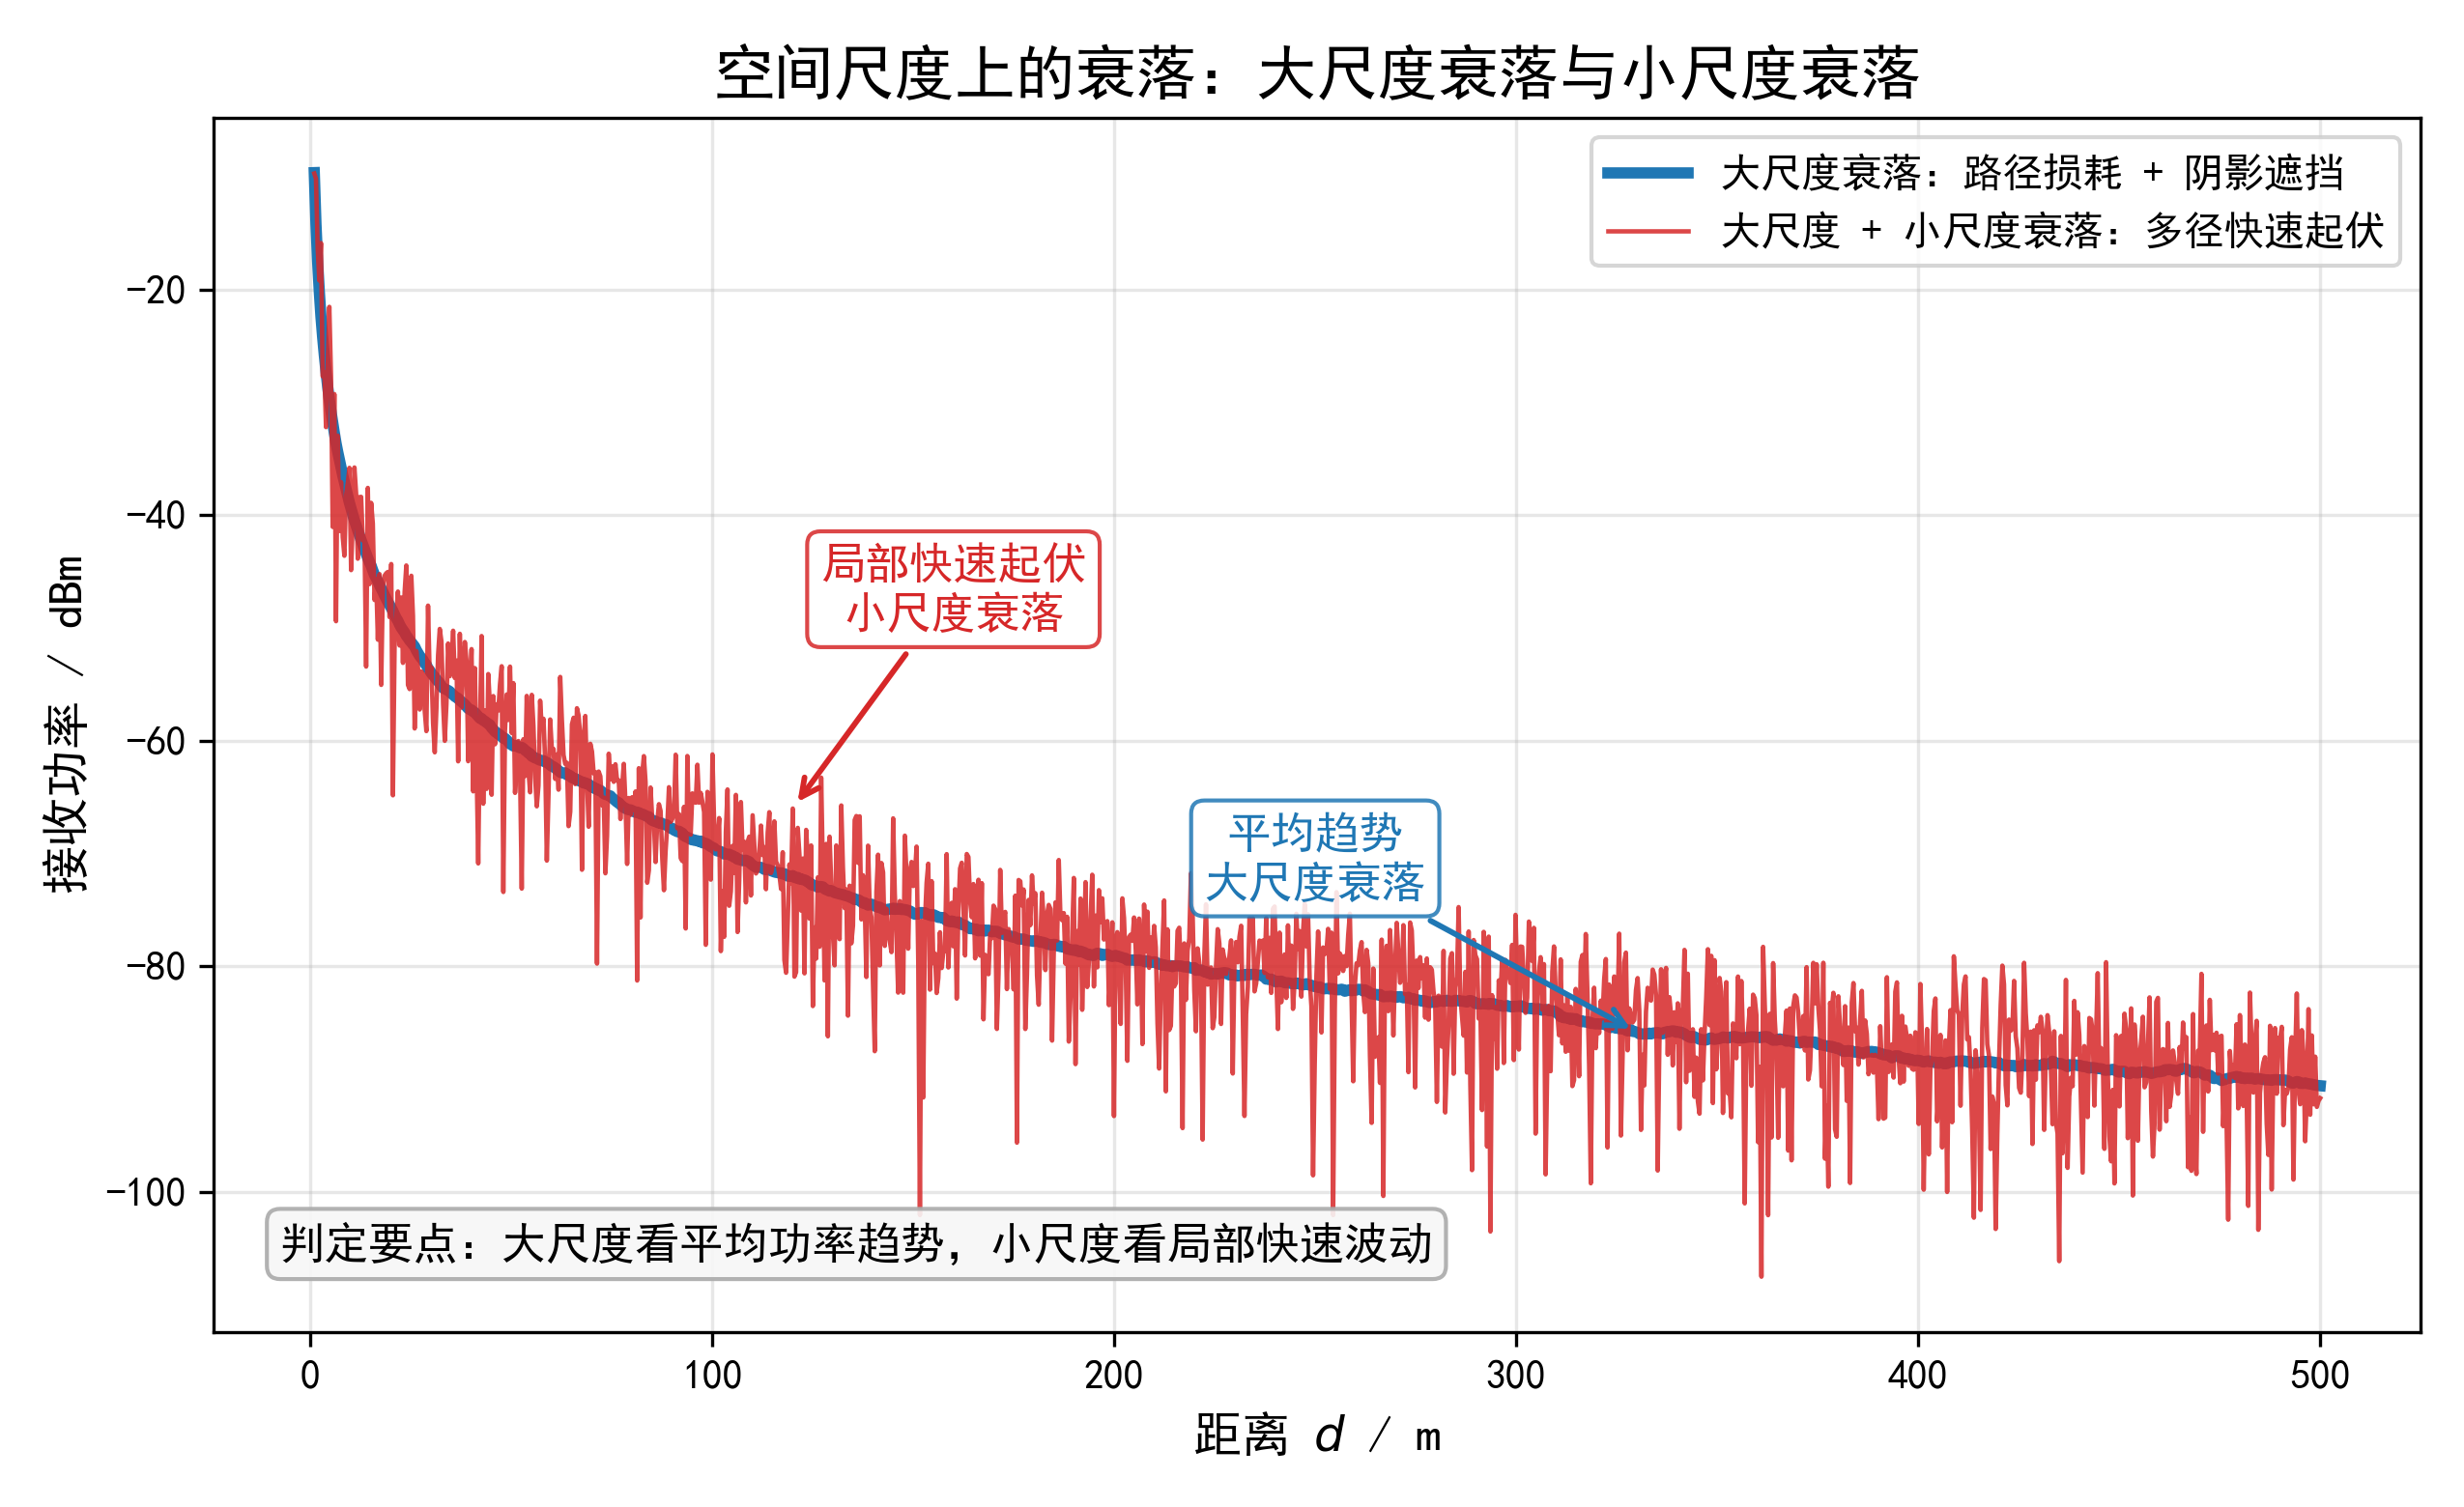
\includegraphics[width=0.75\textwidth]{figures/chapter1/fig_fading.png}
    \caption{大尺度衰落与小尺度衰落对比图}
    \label{fig:spatial-fading}
\end{figure}
\noindent\textbullet\quad\textbf{从时间维度看：多普勒频移、相干时间与快慢衰落}

从时间维度看，
衰落与信道的时变特性密切相关。
当发射端、接收端或环境中的散射体存在相对运动时，
各传播路径上的幅度和相位可能随时间发生变化，
从而使信道呈现非平稳或时变特性。
其中，
由相对运动引起的相位变化会表现为多普勒频移。
最大多普勒频移通常可以写为
\begin{equation}
    f_D
    =
    \frac{v}{\lambda}
    =
    \frac{v f_c}{c},
    \label{eq:maximum-doppler-shift}
\end{equation}
其中，
\(v\) 表示相对速度，
\(\lambda\) 表示载波波长，
\(f_c\) 表示载波频率，
\(c\) 表示光速。
由式~\eqref{eq:maximum-doppler-shift} 可以看出，
在相同载波频率下，
相对速度越高，
多普勒频移越大；
在相同运动速度下，
载波频率越高、波长越短，
多普勒效应也越明显。
因此，
高速移动场景和毫米波、太赫兹等高频通信场景中，
信道随时间变化的问题更加突出。

为了描述信道在时间上的稳定程度，
通常引入\textbf{相干时间} \(T_c\) 的概念。
相干时间可以理解为信道在时间上近似保持不变的时间尺度。
一般而言，
相干时间与最大多普勒频移近似成反比，
即
\begin{equation}
    T_c
    \propto
    \frac{1}{f_D}.
    \label{eq:coherence-time}
\end{equation}
多普勒频移越大，
相干时间越短，
说明信道变化越快；
多普勒频移越小，
相干时间越长，
说明信道在较长时间内更加稳定。

在此基础上，
可以理解慢衰落和快衰落的区别。
设信号的符号持续时间为 \(T_s\)。

\textbf{慢衰落}是指信道变化相对于信号变化较慢的情形。
如果 \(T_s \ll T_c\)，
则在一个符号周期内信道基本保持不变，
接收信号可以近似看作经过一个相对固定的信道传输。
这种情况下，
信道变化主要体现在较长时间尺度上，
通常称为慢衰落。

\textbf{快衰落}是指信道变化相对于信号变化较快的情形。
如果 \(T_s\) 与 \(T_c\) 接近，
甚至大于 \(T_c\)，
则信道可能在一个符号周期内发生明显变化，
从而使接收信号在符号内部也经历时变信道影响。
这种情况下，
接收端的同步、信道估计和均衡会更加困难，
通常称为快衰落。

因此，
快衰落和慢衰落并不是单纯由“移动速度快不快”决定的绝对概念，
而是由信道变化时间尺度与信号时间尺度之间的相对关系决定的。

\noindent\textbullet\quad\textbf{从频率维度看：时延扩展、相干带宽与频率选择性}

从频率维度看，
衰落与多径时延扩展密切相关。
在多径传播中，
不同路径具有不同的传播距离，
因此到达接收端的时间并不完全相同。
多个路径分量在时延轴上分散开来的现象称为时延扩展。
常用均方根时延扩展 \(\tau_{\mathrm{rms}}\)
描述多径能量在时延轴上的分散程度。
时延扩展越大，
说明不同多径分量之间的到达时间差越明显，
信道频率响应随频率变化的起伏通常也越强。

为了描述信道在频率上的相关范围，
通常引入\textbf{相干带宽} \(B_c\) 的概念。
相干带宽可以理解为信道频率响应在频率上近似保持一致的频率范围。
一般而言，
相干带宽与均方根时延扩展近似成反比，
即
\begin{equation}
    B_c
    \propto
    \frac{1}{\tau_{\mathrm{rms}}}.
    \label{eq:coherence-bandwidth}
\end{equation}
时延扩展越大，
相干带宽越小，
说明信道在较窄的频率范围内就可能发生明显变化；
时延扩展越小，
相干带宽越大，
说明较宽频带内的信道响应仍可能比较相似。

\textbf{平坦衰落}是指信号带宽 \(B\)
远小于相干带宽 \(B_c\) 时的衰落形式，
即 \(B \ll B_c\)。
在这种情况下，
信号带宽内的各个频率分量经历近似相同的信道响应，
整个信号频带可以近似看作受到同一个复数信道系数的影响。
因此，
平坦衰落虽然会改变信号的整体幅度和相位，
但通常不会使不同频率分量产生明显不同的失真。

\textbf{频率选择性衰落}是指信号带宽 \(B\)
与相干带宽 \(B_c\) 接近，
或者 \(B > B_c\) 时的衰落形式。
在这种情况下，
不同频率分量可能经历不同的幅度衰减和相位变化，
因此接收信号会出现频域上的非均匀失真。
频率选择性衰落是宽带无线通信中的重要问题，
也是 OFDM 多载波传输技术的重要动机之一。
OFDM 通过将宽带信号划分为多个窄带子载波，
使每个子载波上的信道近似表现为平坦衰落信道，
从而降低均衡和接收处理的复杂度。

需要强调的是，
大尺度衰落、小尺度衰落、慢衰落、快衰落、
平坦衰落和频率选择性衰落并不是彼此互斥的分类。
它们只是从不同观察角度描述无线信道的变化特性：
空间尺度关注接收信号随位置变化的趋势，
时间维度关注信道随时间变化的快慢，
频率维度关注信道对不同频率分量的不同影响。
一个实际无线信道可能同时受到路径损耗、阴影遮挡、多径叠加、
移动性和频率选择性等因素的影响。

对于传统通信系统而言，
衰落主要体现为影响可靠传输和链路质量的不利因素；
而对于 ISAC 系统而言，
衰落背后的时延、多普勒、角度和路径增益等物理量，
也可能携带目标运动、空间结构和环境状态等感知信息。
因此，
在 ISAC 中理解衰落不仅是为了补偿信道影响，
也是为了进一步利用无线传播过程中的环境信息。

上述衰落概念分别从空间尺度、时间变化和频率响应等角度描述无线信道的不同特性。
为了便于对比和记忆，
表~\ref{tab:fading-types-comparison} 对常见衰落类型的主要来源、
判定要素和直观含义进行了总结。
在实际无线环境中，
这些衰落现象往往会同时存在，
共同影响通信链路质量和 ISAC 系统的感知性能。
\begin{table}[htbp]
    \centering
    \caption{不同衰落类型的对比}
    \label{tab:fading-types-comparison}
    \renewcommand{\arraystretch}{1.35}
    \begin{tabularx}{\textwidth}{p{0.13\textwidth} p{0.16\textwidth} X X X}
        \hline
        \textbf{观察维度}
        &
        \textbf{衰落类型}
        &
        \textbf{主要来源}
        &
        \textbf{判定要素}
        &
        \textbf{直观理解}
        \\
        \hline

        空间尺度
        &
        大尺度衰落
        &
        路径损耗、阴影遮挡、地形与建筑物阻挡
        &
        接收信号平均功率随位置或距离缓慢变化
        &
        信号整体变弱或被遮挡
        \\

        空间尺度
        &
        小尺度衰落
        &
        多径分量的相干叠加
        &
        接收信号在短距离或短时间内快速起伏
        &
        移动很短距离，信号也可能明显增强或减弱
        \\

        时间维度
        &
        慢衰落
        &
        低移动性、较小多普勒频移
        &
        \(T_s \ll T_c\)
        &
        一个符号周期内信道近似不变
        \\

        时间维度
        &
        快衰落
        &
        高移动性、较大多普勒频移或快速变化的散射环境
        &
        \(T_s \gtrsim T_c\)
        &
        一个符号周期内信道已经明显变化
        \\

        频率维度
        &
        平坦衰落
        &
        较小的多径时延扩展
        &
        \(B \ll B_c\)
        &
        整个信号带宽内的频率分量经历近似相同的信道
        \\

        频率维度
        &
        频率选择性衰落
        &
        较大的多径时延扩展
        &
        \(B \gtrsim B_c\)
        &
        不同频率分量经历不同幅度衰减和相位变化
        \\
        \hline
    \end{tabularx}
\end{table}


\paragraph{通信质量指标分类}

前面讨论的路径损耗、多径传播、衰落、噪声和干扰，
都会改变接收端观测到的信号质量。
为了评价这些因素对信息传输的影响，
通信系统需要引入一系列质量指标。
不同指标关注的层面并不相同：
有些指标描述接收信号本身的质量，
有些指标衡量信息恢复是否可靠，
还有一些指标反映系统在有限频谱和时间资源下能够传输多少有效信息。
因此，
通信质量指标可以大致分为三类：
\textbf{链路质量指标}、\textbf{可靠性指标}和\textbf{效率指标}。

\textbf{链路质量指标}主要用于描述接收端有用信号相对于噪声或干扰的强弱关系，
典型指标包括信噪比（signal-to-noise ratio, SNR）
和信干噪比（signal-to-interference-plus-noise ratio, SINR）。
信噪比定义为有用信号功率与噪声功率之比，
即
\begin{equation}
    \mathrm{SNR}
    =
    \frac{P_s}{P_n},
    \label{eq:snr-definition}
\end{equation}
其中，
\(P_s\) 表示接收端的有用信号功率，
\(P_n\) 表示噪声功率。
若噪声功率谱密度为 \(N_0\)，
系统带宽为 \(B\)，
则噪声功率常可写为
\begin{equation}
    P_n
    =
    N_0 B.
    \label{eq:noise-power-bandwidth}
\end{equation}
因此，
在接收信号功率固定的情况下，
带宽增大会引入更多噪声功率，
从而可能降低 SNR。
一般来说，
发射功率越高、路径损耗越小、
天线增益或波束增益越大，
接收信号功率越强，
SNR 越高；
而噪声功率越大，
SNR 越低。

在实际系统中，
接收端受到的非期望成分往往不只有噪声，
还包括来自其他用户、邻近小区、同频系统或共享频谱设备的干扰。
因此，
信干噪比比 SNR 更适合描述实际通信链路质量，
其定义为
\begin{equation}
    \mathrm{SINR}
    =
    \frac{P_s}{P_i + P_n},
    \label{eq:sinr-definition}
\end{equation}
其中，
\(P_i\) 表示干扰功率。
当干扰功率较小时，
SINR 近似退化为 SNR；
当系统处于干扰受限状态时，
即使提高发射功率，
通信性能也可能提升有限，
此时干扰协调、资源调度、功率控制和波束成形等技术会变得更加重要。
对于 ISAC 系统而言，
SINR 的意义更加突出，
因为通信与感知功能可能共享时间、频率、空间和功率资源，
通信信号、感知回波、杂波以及其他用户信号之间
可能形成更加复杂的相互影响。

\textbf{可靠性指标}用于衡量接收端能否正确恢复发送端的信息。
最常见的可靠性指标是误码率（bit error rate, BER），
其定义为错误比特数与总传输比特数之比：
\begin{equation}
    \mathrm{BER}
    =
    \frac{N_{\mathrm{error}}}{N_{\mathrm{total}}},
    \label{eq:ber-definition}
\end{equation}
其中，
\(N_{\mathrm{error}}\) 表示接收端判决错误的比特数，
\(N_{\mathrm{total}}\) 表示总传输比特数。
BER 越低，
说明通信链路的可靠性越高。
通常情况下，
SNR 或 SINR 越高，
接收端越容易区分不同调制符号，
BER 越低；
而当衰落严重、干扰增强或噪声功率增大时，
BER 往往会上升。

误码率还与调制方式和信道编码密切相关。
在相同 SNR 条件下，
高阶调制方式能够在每个符号中携带更多比特，
但星座点之间的距离更近，
因此通常更容易受到噪声和干扰影响；
低阶调制方式虽然频谱效率较低，
但鲁棒性更强。
信道编码可以通过引入冗余帮助接收端检测和纠正错误，
从而降低误码率，
但也会带来一定的速率开销。
在实际移动通信系统中，
还常使用块错误率（block error rate, BLER）
描述一个传输块是否被正确解码。
相比 BER，
BLER 更接近链路自适应、重传机制和实际吞吐率的评价需求。

\textbf{效率指标}用于衡量通信系统在有限资源下传输信息的能力。
最基本的速率指标是数据率，
表示单位时间内传输的信息比特数。
在理想高斯信道中，
信道容量可以作为理论上限参考，
其形式为
\begin{equation}
    C
    =
    B \log_2
    \left(
        1+\mathrm{SNR}
    \right),
    \label{eq:capacity-snr}
\end{equation}
其中，
\(C\) 表示信道容量，
\(B\) 表示系统带宽。
如果考虑干扰影响，
也常将 SNR 替换为 SINR，
写作
\begin{equation}
    C
    =
    B \log_2
    \left(
        1+\mathrm{SINR}
    \right).
    \label{eq:capacity-sinr}
\end{equation}
式~\eqref{eq:capacity-snr} 和式~\eqref{eq:capacity-sinr} 表明，
容量与带宽和链路质量都有关。
增大带宽可以提供更多频率资源，
提高 SNR 或 SINR 可以提升单位带宽内可承载的信息量。
但是，
容量随 SNR 或 SINR 的增长呈对数关系，
因此在高信噪比区域，
继续提高功率带来的速率增益会逐渐减小。

吞吐率更接近实际系统中成功传输的信息量。
它可以理解为单位时间内被接收端正确接收的有效数据量，
常写为
\begin{equation}
    R_{\mathrm{throughput}}
    =
    \frac{N_{\mathrm{success}}}{T},
    \label{eq:throughput-definition}
\end{equation}
其中，
\(N_{\mathrm{success}}\) 表示在时间 \(T\) 内成功接收的信息比特数。
若用 \(R\) 表示名义传输速率，
用 BLER 表示块错误率，
则实际吞吐率可近似表示为
\begin{equation}
    R_{\mathrm{throughput}}
    \approx
    R
    \left(
        1-\mathrm{BLER}
    \right).
    \label{eq:throughput-bler}
\end{equation}
这一表达式说明，
较高的名义速率并不一定意味着较高的实际吞吐率。
如果信道条件较差，
导致错误率或重传概率升高，
实际成功传输的数据量可能反而下降。

频谱效率（spectral efficiency）用于衡量单位带宽内能够传输多少信息，
通常定义为
\begin{equation}
    \eta
    =
    \frac{R}{B},
    \label{eq:spectral-efficiency-definition}
\end{equation}
单位为 bit/s/Hz。
如果以信道容量作为理想参考，
则频谱效率可以写为
\begin{equation}
    \eta
    =
    \log_2
    \left(
        1+\mathrm{SNR}
    \right),
    \label{eq:spectral-efficiency-snr}
\end{equation}
或者在考虑干扰时写为
\begin{equation}
    \eta
    =
    \log_2
    \left(
        1+\mathrm{SINR}
    \right).
    \label{eq:spectral-efficiency-sinr}
\end{equation}
频谱效率越高，
说明系统在有限频谱资源中传输信息的能力越强。
在频谱资源日益紧张的背景下，
频谱效率是评价无线通信系统的重要指标之一。
对于 ISAC 而言，
频谱效率还具有更特殊的意义：
ISAC 希望通过通信与感知共享频谱、硬件和波形资源，
在不额外占用大量频谱的情况下同时支持信息传输和环境感知。
因此，
频谱效率不仅反映通信链路本身的资源利用能力，
也与通感资源复用和系统整体效率密切相关。

在实际系统中，
这些通信质量指标之间存在清晰的逻辑关系。
路径损耗、多径、衰落、噪声和干扰
首先影响接收端的 SNR 或 SINR；
SNR 或 SINR 进一步决定解调和译码的可靠性，
并体现在 BER 或 BLER 等指标上；
可靠性又会影响实际吞吐率，
而在给定带宽下，
有效传输速率进一步决定频谱效率。
因此，
可以将通信质量指标理解为从“接收信号质量”到“信息恢复可靠性”，
再到“资源利用效率”的逐层度量。
对于 ISAC 系统而言，
这些指标仍然是评价通信性能的基础，
同时也为后续讨论通信与感知之间的性能权衡、
资源分配和联合优化提供了重要依据。

\paragraph{信道状态信息的定义、获取与作用}

通信系统若要根据无线信道状态进行接收处理和传输优化，
首先需要获得对当前信道的描述信息，
这类信息通常称为\textbf{信道状态信息}
（channel state information, CSI）。
CSI 反映了信号在传播过程中受到的幅度衰减、
相位旋转、时延扩展、频率选择性以及空间方向等影响。
换言之，
CSI 可以看作通信系统对无线信道当前状态的数学描述。

CSI 的具体形式与系统结构有关。
在单天线窄带系统中，
CSI 可以简化为一个复数信道系数
\begin{equation}
    h
    =
    |h|e^{j\phi},
    \label{eq:csi-siso-coefficient}
\end{equation}
其中，
\(|h|\) 描述信号幅度的变化，
\(\phi\) 描述信号相位的变化。
在 OFDM 系统中，
CSI 通常表示为不同子载波上的频域信道响应
\begin{equation}
    H[k],
    \label{eq:csi-ofdm-subcarrier}
\end{equation}
其中，
\(k\) 表示子载波索引，
\(H[k]\) 描述第 \(k\) 个子载波上的信道幅度和相位变化。
在 MIMO 系统中，
CSI 则常表示为信道矩阵
\begin{equation}
    \mathbf{H},
    \label{eq:csi-mimo-matrix}
\end{equation}
其矩阵元素描述不同发射天线与接收天线之间的空间信道关系。
由此可见，
CSI 并不固定为某一种形式，
但其核心作用都是描述无线信道对发射信号的影响。

CSI 通常通过导频或参考信号进行估计。
发送端在预定的时间、频率或空间资源位置发送接收端已知的导频符号，
接收端根据导频的已知发送值和对应接收值估计信道。
在不同系统和假设条件下，
可以采用不同的信道估计算法，
例如最小二乘估计（least squares, LS）、
线性最小均方误差估计
（linear minimum mean square error, LMMSE）
以及结合插值、滤波或压缩感知的方法。
在 OFDM 系统中，
CSI 往往需要在多个导频子载波上获得，
再通过频域或时域插值估计其他资源位置上的信道响应；
在 MIMO 系统中，
还需要估计不同发射天线和接收天线之间的信道矩阵。

CSI 的获取方式还与双工方式有关。
在 FDD 系统中，
上行和下行通常使用不同频段，
二者信道不完全相同，
因此接收端估计下行 CSI 后，
通常需要通过反馈链路将信道质量或预编码相关信息反馈给发射端。
在 TDD 系统中，
上行和下行使用同一频段的不同时隙，
理想情况下无线传播信道具有互易性，
因此基站可以根据上行导频估计信道，
并将其用于下行传输设计。
不过，
在实际系统中，
信道互易性还会受到射频前端差异的影响，
因此通常需要进行一定的校准。

CSI 在通信系统设计中具有基础作用。
首先，
接收端可以利用 CSI 进行信道均衡，
补偿信道引起的幅度衰减、相位旋转和频率选择性失真，
从而提高解调和译码的可靠性。
其次，
发射端或系统调度器可以根据信道质量进行自适应调制编码：
当信道条件较好时，
可以采用高阶调制和较高编码率以提升速率；
当信道条件较差时，
则可以采用低阶调制和更强的信道编码以保证可靠性。
此外，
CSI 还可以用于功率控制、用户调度、资源分配以及重传策略设计。

在 MIMO 系统中，
CSI 的作用更加突出。
发射端或接收端可以根据信道矩阵设计波束成形和预编码权重，
使发射能量尽可能集中到目标用户方向，
同时抑制对其他用户的干扰。
对于多用户 MIMO 系统，
CSI 还可以帮助系统判断哪些用户适合在同一时频资源上进行空间复用，
从而提高系统容量和频谱效率。
可以说，
CSI 是通信系统从固定传输走向自适应传输的重要基础。

从 ISAC 的角度看，
CSI 的意义进一步扩展。
在传统通信系统中，
CSI 主要用于补偿信道影响、
提高通信可靠性和传输效率；
而在 ISAC 系统中，
CSI 本身也可能包含目标和环境信息。
例如，
信道中的时延信息可能对应传播路径长度或目标距离，
多普勒频移可能反映目标或散射体的相对运动，
角度信息可能对应目标方向或空间结构，
路径增益和反射特性则可能反映目标散射强度或环境材料特征。
因此，
CSI 不仅是通信链路自适应设计的依据，
也可能成为 ISAC 系统感知环境和理解目标状态的重要入口。

由此可以看出，
CSI 将无线信道的物理特性与通信系统设计连接起来。
对于通信而言，
CSI 用于适应和补偿信道；
对于 ISAC 而言，
CSI 还可以帮助系统从信道变化中提取环境、目标和运动信息。
这也是后续讨论 OFDM 信道估计、MIMO 波束成形
以及通信-感知联合处理时需要反复依赖的基础概念。
  % 包含第一章绪论
% 可以继续 include chapter2, chapter3...

% --- 附录部分 ---
\appendix
% \appendix 命令会将章节编号从 1, 2, 3 转换为 A, B, C
% \chapter{数学推导与补充证明}
% \section{信道模型的推导细节}
% 这里是附录 A 的内容... % 比如：相关的数学推导或额外数据

% --- 后记部分 ---
\backmatter 

% \backmatter 会关闭章节编号，但依然会将大标题加入目录（适用于参考文献、致谢、索引等）

% 1. 设置参考文献的格式（IEEE 格式会自动将引用按数字 [1], [2] 排序）
\bibliographystyle{ieeetr}

% 2. 告诉 LaTeX 你的参考文献数据库在哪里（不需要加 .bib 后缀）
\bibliography{bib/references}

\end{document}